\documentclass[12pt,letterpaper]{report}
\usepackage{natbib}
\usepackage{geometry}
\usepackage{fancyhdr}
\usepackage{afterpage}
\usepackage{graphicx}
\usepackage{amsmath,amssymb,amsbsy}
\usepackage{dcolumn,array}
\usepackage{tocloft}
\usepackage{asudis}
\usepackage[pageanchor=true,plainpages=false,pdfpagelabels,bookmarks,bookmarksnumbered,colorlinks=true,linkcolor=black,anchorcolor=black,citecolor=black,filecolor=black,menucolor=black,runcolor=black,urlcolor=black]{hyperref}
\begin{document}
%-----------------------front matter
\pagenumbering{roman}
\title{A Visual Analytics Process for Exploring Risk and Vulnerability in International Food Trade Networks}
\author{Travis Seville}
\degreeName{Master of Science}
\paperType{Thesis}
\defensemonth{November}
\defenseyear{2017}
\gradmonth{December}
\gradyear{2017}
\chair{Ross Maciejewski}
\memberOne{I-Han Hsiao}
\memberTwo{Shade Shutters}
\maketitle
\doublespace
\begin{abstract}
	\label{abstractChapter}
	The rise in globalization has led to regional climate events having an increased effect on global food security. These indirect first- and second-order effects are generally geographically disparate from the region experiencing the climate event. Without understanding the topology of the food trade network, international aid may be naively directed to the countries directly experiencing the climate event and not to countries that will face potential food insecurity due to that event. This thesis focuses on the development of a visual analytics system for exploring second-order effects of climate change under the lens of global trade. In order to visualize how climate change impacts the world trade network of agricultural goods I have developed an interactive data visualization platform for analysis of the interaction between climate events and the trade network. The proposed visual analytics system focuses on visualizing current trade dependencies at a more granular level than the currently available tools and to aid in the identification of future vulnerabilities. To demonstrate the applicability of the tool, two case studies are described. The first case study focuses on the Chinese drought of 2011 and its impact on the global trade network and food security. The second case study will model the potential impact of a climate event affecting production in the United States, a large supplier of corn, to demonstrate the potential consequence of cascading effects in the global trade network.
\end{abstract}
%\dedicationpage{}
\label{ackChapter}
I dedicate this thesis to my family; for their support and consistent motivation.\par
My parents. Without them, none of this would have been possible.\par
My wife, Nichole, who pushed me and always held me accountable.\par
My children, Lacy, Lia and Logan, who inspired me.\par

\tableofcontents
% This puts the word "Page" right justified above everything else.
\addtocontents{toc}{~\hfill Page\par}
% Asking LaTeX for a new page here guarantees that the LOF is on a separate page
% after the TOC ends.
\newpage
% Making the LOT and LOF "parts" rather than chapters gets them indented at
% level -1 according to the chart: top of page 4 of the document at
% ftp://tug.ctan.org/pub/tex-archive/macros/latex/contrib/tocloft/tocloft.pdf
\addcontentsline{toc}{part}{LIST OF TABLES}
\renewcommand{\cftlabel}{Table}
\listoftables
% This gets the headers for the LOT right on the first page.  Subsequent pages
% are handled by the fancyhdr code in the asudis.sty file.
\addtocontents{lot}{Table~\hfill Page \par}
\newpage
\addcontentsline{toc}{part}{LIST OF FIGURES}
\addtocontents{toc}{CHAPTER \par}
\renewcommand{\cftlabel}{Figure}
% This gets the headers for the LOF right on the first page.  Subsequent pages
% are handled by the fancyhdr code in the asudis.sty file.
\addtocontents{lof}{Figure~\hfill Page \par}
\listoffigures
%-----------------------body
\doublespace
\pagenumbering{arabic}
%\chapter{Notes}
ASSESSING AGRICULTURAL VULNERABILITY TO CLIMATE CHANGE IN THE NORDIC COUNTRIES – AN INTERACTIVE GEOVISUALIZATION APPROACH: ~\cite{wirehn2016assessing}\\
\textit{Nordic agriculture must adapt to climate change to reduce vulnerability and exploit potential opportunities. Integrated assessments can identify and quantify vulnerability in order to recognize these adaptation needs. This study presents a geographic visualization approach to support the interactive assessment of agricultural vulnerability to climate change. We have identified requirements for increased transparency and reflexivity in vulnerability assessments, arguing that these can be met by geographic visualization. A conceptual framework to support the integration of geographic visualization for vulnerability assessments has been designed and applied for the development of AgroExplore, an interactive tool for assessing agricultural vulnerability to climate change in Sweden. To open up the black box of composite vulnerability indices, AgroExplore enables the user to select, weight, and classify relevant indicators into sub-indices of exposure, sensitivity, and adaptive capacity. This enables the exploration of underlying indicators and factors determining vulnerability in Nordic agriculture.}\\
Defines potential similar workflows for how manipulation of the indicators would propogate into vulnerability indices. Social indicators may be important as well. Number of farmers and other employment in agriculture. Where can we get statistics for these? Extension of this agricultural vulnerability tool into the economic and trade network realms. What is the direct connection between agricultural vulnerability and trade network stability or vulnerability. There a lots of potential references here.\\
\\
ASSESSMENT OF COMPOSITE INDEX METHODS FOR AGRICULTURAL VULNERABILITY TO CLIMATE CHANGE:~\cite{wirehn2015assessment}\\
\textit{A common way of quantifying and communicating climate vulnerability is to calculate composite indices from indicators, visualizing these as maps. Inherent methodological uncertainties in vulnerability assessments, however, require greater attention. This study examines Swedish agricultural vulnerability to climate change, the aim being to review various indicator approaches for assessing agricultural vulnerability to climate change and to evaluate differences in climate vulnerability depending on the weighting and summarizing methods. The reviewed methods are evaluated by being tested at the municipal level. Three weighting and summarizing methods, representative of climate vulnerability indices in general, are analysed. The results indicate that 34 of 36 method combinations differ significantly from  each other. We argue that representing agricultural vulnerability in a single composite index might be insufficient to guide climate adaptation. We emphasize the need for further research into how to measure and visualize agricultural vulnerability and into how to communicate uncertainties in both data and methods.}\\
There are vulnerability indicators with descriptions here that may be useful. Groups of vulnerability indices: exposure, sensitivity, adaptive capacity. These groups will be possibly different for different regions. At least the index value will be different for different region. The indicators in each group will stay the same, but we can use it as a means of grouping the variables for a starting point. What I mean is possibly sliders that change the composite index of each group, instead of as a whole or as the individual indices. Adaptive capacity should remain static (or at least independent of climate singularities) in future predictions, but could be manipulated for exploration. Good indexing of the correlation between indicator and whether it has a positive of negative impacted on the overall vulnerability index.\\
\\
INDICATORS OF VULNERABILITY AND ADAPTIVE CAPACITY: ~\cite{hinkel2011indicators}\\
\textit{The issue of 'measuring' climate change vulnerability and adaptive capacity by means of indicators divides policy and academic communities. While policy increasingly demands such indicators an increasing body of literature criticises them. This misfit results from a twofold confusion. First, there is confusion about what vulnerability indicators are and which arguments are available for building them. Second, there is confusion about the kinds of policy problems to be solved by means of indicators. This paper addresses both sources of confusion. It first develops a rigorous conceptual framework for vulnerability indicators and applies it to review the scientific arguments available for building climate  change vulnerability indicators. Then, it opposes this availability with the following six diverse types of problems that vulnerability indicators are meant to address according to the literature: (i) identification of mitigation targets; (ii) identification of vulnerable people, communities, regions, etc.; (iii) raising awareness; (iv) allocation of adaptation funds; (v) monitoring of adaptation policy; and (vi) conducting scientific research. It is found that vulnerability indicators are only appropriate for addressing the second type of problembut only at local scales, when systems can be narrowly defined and inductive arguments can be built. For the other five types of problems, either vulnerability is not the adequate concept or vulnerability indicators are not the adequate methodology. I conclude that both the policy and academic communities should collaboratively attempt to use a more specific terminology for speaking about the problems addressed and the methodologies applied. The one-size-fits-all vulnerability label is not sufficient. Speaking of 'measuring' vulnerability is particularly misleading, as this is impossible and raises false expectations.}\\
Vulnerability is a measure of possible future harm. What are measures in the realm of trade networks. Are we talking merely profit or the overall economic well being of a region. There is not a real good scientific definition that provides guidance for designing a methodology. This paper will be useful in structuring our definition of vulnerability, as it seems to be a common theme that it is difficult to define. Reread the challenges involved in developing indicators. Distinguishing between harm and vulnerability. Harm indicators are a current state; good or bad state based on normative judgements that do not include the forward-looking aspect. Vulnerability makes the distinction of looking forward aspect as well as defining harm. Using normative arguments in the development of indicators means using (individual or collective) value judgements. Paper poses a large number of questions to ask when consider whether an indicator should be presented. Could use it to validate our indicator selections.\\
\\
INTEGRATING SOCIAL VULNERABILITY INTO WATER MANAGEMENT: ~\cite{downing2006integrating}\\
\textit{The vulnerability of humans related to their use of water has also become a widespread concern, related to climate change, flood and drought hazards, and poverty. A profusion of definitions remains characteristic of vulnerability research and applications. Nevertheless, progression in the past decade toward a vulnerability/adaptation science has recognised six key attributes of social vulnerability. Each implies different methodological approaches:
\begin{enumerate} \item Vulnerability is the differential exposure to stresses experienced or anticipated by different exposure units. \item Vulnerability is a dynamic process, changing on a variety of inter-linked time scales.
	\item Social vulnerability is rooted in the actions and multiple attributes of human actors.
	\item Social networks drive and bound vulnerability in the social, economic, political and
	environmental interactions.
	\item Vulnerability is constructed simultaneously on more than one scale.
	\item Multiple stresses are inherent in integrated vulnerability of peoples, places and systems.
\end{enumerate}
Building upon a typical water planning approach (such as WEAP), four progressions are proposed in understanding vulnerability: (1) introduce differential social and economic vulnerability to catchment planning models; (2) capture the dynamic element of vulnerable groups and their relationship to water resources and catchment or regional planning; (3) represent the multiple attributes of vulnerable groups and make the link to their ability to respond to stresses and threats; and (4) represent the decisions of actors (the managers and vulnerable groups) in the construction of adaptive systems (i.e., in the reduction of future vulnerability). The basic elements of a variety of water resource vulnerability recipes are reviewed.}\\
Notes\\
\\
NODETRIX: ~\cite{henry2007nodetrix}\\
\textit{The need to visualize large social networks is growing as hardware capabilities make analyzing large networks feasible and many new data sets become available. Unfortunately, the visualizations in existing systems do not satisfactorily resolve the basic dilemma of being readable both for the global structure of the network and also for detailed analysis of local communities. To address this problem, we present NodeTrix, a hybrid representation for networks that combines the advantages of two traditional representations: node-link diagrams are used to show the global structure of a network, while arbitrary portions of the network can be shown as adjacency matrices to better support the analysis of communities. A key contribution is a set of interaction techniques. These allow analysts to create a NodeTrix visualization by dragging selections to and from node-link and matrix forms, and to flexibly manipulate the NodeTrix representation to explore the dataset and create meaningful summary visualizations of their findings. Finally, we present a case study applying NodeTrix to the analysis of the InfoVis 2004 coauthorship dataset to illustrate the capabilities of NodeTrix as both an exploration tool and an effective means of communicating results.}\\
Technique was to split the visualization based on the two different densities of data at different spectrums. Locally the information was dense and therefore warranted a matrix representation. The community connections however were sparse and were better represented with a node-link diagram. This novel approach combined the two visualizations and allowed for user manipulation to condense the nodes into matrices.
What I garnered from this paper was the different types of clusters and what visualizations lend best represent each density. The term “small-world networks” was introduced to me as an intermediate category of data that has both sparse and dense clusters. These are common in data from social networks. Adjacent matrices are well suited for dense data such as our data set of exports from a county. However, there may be many countries with many different values that may not lend itself well to such a simplistic view model. We need to be able to represent quantity in a better fashion, and that’s why flow maps would be better suited than matrices. The paper says “matrix representations ease community analysis, but hinder identification of important global structures” which is most definitely pertinent to our data.
There was a lot of useful information on editing and information regarding user interface overall. The manipulation of matrices and nodes seemed intuitive and as I was reading I found myself having ideas that they presented shortly after.\\
\\
REDUCING SNAPSHOTS TO POINTS: ~\cite{van2016reducing}\\
\textit{We propose a visual analytics approach for the exploration and analysis of dynamic networks. We consider snapshots of the network as points in high-dimensional space and project these to two dimensions for visualization and interaction using two juxtaposed views: one for showing a snapshot and one for showing the evolution of the network. With this approach users are enabled to detect stable states, recurring states, outlier topologies, and gain knowledge about the transitions between states and the network evolution in general. The components of our approach are discretization, vectorization and normalization, dimensionality reduction, and visualization and interaction, which are discussed in detail. The effectiveness of the approach is shown by applying it to artificial and real-world dynamic networks.}\\
Network evolution is important if we are going to be visualizing current and potential futures states. There are two different basic approaches: time to time and time to space. A key point in creating an effective representation is a balance between fewer images lacking temporal data and many images lacking interpretability. There are two dominant methods for these types of data. Animation, where you see time lapsed by changing visualizations and small multiples where there are point in time visualizations based on a time interval. One the important considerations is mental map preservation. Being able to adjust the quantity and visualizations of data to be able to be effectively retained, either in a session state or more long term. Initially I think animation would be the most appropriate method for visualizing a flow map over a time period. The idea to break up the approach into these 4 steps could be translated to a flow map, this would still need to determined and explored further.\\\textsl{}
\\
TOWARDS A FORMAL FRAMEWORK OF VULNERABILITY TO CLIMATE CHANGE: ~\cite{ionescu2009towards}\\
\textit{There is confusion regarding the notion of “vulnerability” in the climate change scientific community. Recent research has identified a need for formalisation, which would support accurate communication and the elimination of misunderstandings that result from ambiguous interpretations. Moreover, a formal framework of vulnerability is a prerequisite for computational approaches to its assessment. This paper presents an attempt at developing such a formal framework. We see “vulnerability” as a relative concept, in the sense that accurate statements about vulnerability are possible only if one clearly specifies (i) the entity that is vulnerable, (ii) the stimulus to which it is vulnerable and (iii) the preference criteria to evaluate the outcome of the interaction between the entity and the stimulus. We relate the resulting framework to the IPCC conceptualisation of vulnerability and two recent vulnerability studies.}\\
\\
VULNERABILITY: ~\cite{adger2006vulnerability}\\
\textit{This paper reviews research traditions of vulnerability to environmental change and the challenges for present vulnerability research in integrating with the domains of resilience and adaptation. Vulnerability is the state of susceptibility to harm from exposure to stresses associated with environmental and social change and from the absence of capacity to adapt. Antecedent traditions include theories of vulnerability as entitlement failure and theories of hazard. Each of these areas has contributed to present formulations of vulnerability to environmental change as a characteristic of social-ecological systems linked to resilience. Research on vulnerability to the impacts of climate change spans all the antecedent and successor traditions. The challenges for vulnerability research are to develop robust and credible measures, to incorporate diverse methods that include perceptions of risk and vulnerability, and to incorporate governance research on the mechanisms that mediate vulnerability and promote adaptive action and resilience. These challenges are common to the domains of vulnerability, adaptation and resilience and form common ground for consilience and integration.}\\
\\
AGRICULTURAL TRADE NETWORK AND PATTERNS OF ECONOMIC DEVELOPMENT: ~\cite{shutters2012agricultural}\\
There are similarities of agricultural trade network (ATN) with known triad significance profile (TSP) of human social networks; and biological information processing networks to a lesser degree.  Is there a separate superfamily of TSPs for ATNs? Learned what in-degree and out-degree definitions of nodes are. (1, 0) indicates 1 incoming edge (imports) and 0 outgoing edges (exports).
Triads were the main take away from this paper. There are direct connections that can be made with my thesis. Some thinking points that came up were how we would effectively visualize the triads. Is this is an effective method for how we want to display the related information? 
There are special cases of the 18 ‘isolated’ countries when it comes to trade networks. Do we need to factor this in when visualizing our information?  Should the prediction algorithms and the filtering take these into account? Are we able to predict with changes to virtual water supply or climate change singularities that a country would enter or exit this categorization? Can we determine what steps a country would need to take to get themselves out of this isolation group?
It would be good to review the work done on the global virtual water trade network reference 10 in this paper.\\
\\
A NETWORK APPROACH TO DIVISION OF LABOR IN ANTS: ~\cite{networkApproach}\\
This article provided more information and background on triads and in/out-degrees. These associations of nodes, in this case ants giving or receiving signals, provide a different type of possible categorization; specializations. Are there specialized countries with respect to the ATN? Are there countries that are primarily exporters or primarily importers? Is this an indicator of economic status/development as in the ‘Agricultural Trade Network and Patterns of Economic Development’ article? Which triads with respect to ATN are indicators of prominence? How many categories of specialization are there? Which triads are indicative of categorization?
Use this paper as reference for specialization based on triad involvement and more importantly which role (in/out degree) the node is. How many unique nodes that are contained within the triad are deterministic of the role a node takes? For example, is triad 1, topmost node (0, 2) [note, this is incorrectly labeled in the draft paper as (2, 0)] ‘major exporter’ because they are more developed? How does this breakdown based down on virtual water values for different products in the ATN.\\
\\
MOTIF SIMPLIFICATION: ~\cite{dunne2013motif}\\
Due to the large number, as we are seeing with creation of the histograms, of trade links with small values it may be useful to simplify some of clusters if it makes sense visually; e.g. the United States exports to each of the Caribbean islands, it we could show one export link in order to make it less cluttered. There is pseudo-code that may prove useful if this approach is implemented.
There are 3 main types of simplification introduced; fan, connector and clique. The above example would be considered a fan, where one node has edges to each of the others, but not each other. This is done at a binary level, but could be modified to use weighted values. For instance, there could possibly be network links back to the United States in the above example, but if the values (however we determine that; quantity or dollar value) are negligible compared to the main export link we could essentially ignore the return links.
This cluster could also prove useful in defining triads for easier comparison and visualization if the simplifications are relevant enough.\\
\\
INTERNATIONAL TRADE AND FINANCIAL INTEGRATION: ~\cite{schiavo2010international}\\
Three binary data points for nodes are defined; node degree (the number of links maintained by each node), average nearest neighbor degree (the correlation between the degree of a node and the average degree of its partners) and clustering coefficient (the percentage of pairs of i's partners that are connected among themselves). These three node data points are also reciprocated in a weighted fashion based on the relative node strength. In our case this would be the value (quantity or dollar value) of an export link.
This paper uses both import and export values for the edges, creating an undirected graph. This may not be desirable in our analysis. However there is data that supports that the degree of symmetry is large enough to make directed analysis unnecessary. This is the case in both binary and weighted graphs. We need to determine if this is true for specific goods, or am I just misunderstanding their statement. It doesn’t seem to make sense that the US exporting to Nigeria has symmetry with imports from Nigeria. The correlation between node degree and node strength is negative, suggesting that nodes with a small number of links tend to connect to hubs, i.e. to nodes with many partners and suggests that the international trade network is organized as a star-shaped network.\\
\\
CHALLENGING PROBLEMS OF GEOSPATIAL VISUAL ANALYTICS: ~\cite{andrienko2011challenging}\\
Analytic reasoning can be done at two different points; primarily by human analysts or primarily computational. This lends itself to two different types visual interactions; one where the pieces are manipulated by the user and on where the computational methods are manipulated by the user.  The second approach is what I had in mind from the inception of this research. Applications of different kinds of forecasting and prediction algorithms are what would be manipulated by users, not the actual predicted future data. E.g. using X forecasting model would predict N mm of rain in 2020 is manipulating the computational model as opposed to stating there will be M mm of rain in 2020. There are also the techniques of clustering as in Motif Simplification paper, projection, aggregation, pattern extraction and simulation. Simulation is on the techniques I think will be relevant to our project.
Geographical data lends itself well to this two dimensional representation as there is the natural mapping. The quality of data is ever increasing with respect to location. We are going to be utilizing space and time and so the VisMaster findings noted in the paper are pertinent. There is also the interesting application of a countermeasure to the temporal problem. In our application we can also take this into consideration; what if countries started retaining water in an attempt to mitigate ‘drought’ years or the like. Need to bank on the two capabilities of humans; employ previous knowledge (including common sense) and establish associations. The second one we would attempt to enhance.\\
\\
CRITICAL MATERIALS, U.S. IMPORT DEPENDENCE AND RECOMMENDED ACTIONS: ~\cite{silberglitt2015critical}\\
This testimony deals with the pseudo-monopoly of China when it comes to export of certain critical materials and the potential derogatory effects on the U.S. industrial sector. Is there a similar superpower in the agricultural world trade network? Can this be examined based on the number or value of trade links? Using the histograms we created can are we able to answer this question? What can we do to visualize this?
This also introduces some questions that we may need to answer for the ATN. How to recognize a developing pattern, two-tier pricing (see below; initial importer vs second-tier), price spikes or volatility (specifically can we expect volatility with climate singularities?) Are there secondary products that are similar to processed v. unprocessed ore or minerals? How can we identify those?\\
\\
EVOLUTIONARY CONSERVATION OF SPECIES' ROLES IN FOOD WEBS: ~\cite{stouffer2012evolutionary}\\
This contains information on the different unique motif positions. We will use this as a reference when identifying the positions, as well as the triad numerical classification. There is information contribution of a motif and frequency of a motif position to consider when factor the ‘value’ of a position. For instance, in the triad 1, is position 3 more valuable than position 2? Is it assumed that some of the imports to 2 from 3 are then exported to 1, and if so how much? What about for two-way trade links? Can we and if so how do we get this from the data we have? Does this affect the value? Do we need to consider any value adjustment on this second-tier export? Again there is the question of clustering and if there is any value in clustering.\\
\\
\chapter{INTRODUCTION}
\label{introChapter}
Currently, limited research has focused on the inspection of the international food trade network taking into account second-order effects of climate events on the food trade network. These second-order effects are generally geographically disparate from the first-order effects and frequently affect poorer areas that are less capable of dealing with the change, i.e. countries at a higher risk of food insecurity. From my literature study, previous research has summarized this data but has not allowed for a real-time exploration of the international food trade network.\par
This thesis presents a visual analytics system that showcases the indirect effects of a climate event. The region that originally experienced the climate event is generally well recognized and modeled. This tool improves on the current analysis techniques by cascading the consequences of the climate event downstream along the food trade network. This has the potential to identify the level of vulnerability of a country affected by the second-order effects of a climate event. The goal here is to mitigate food security concerns before they result in larger issues by affecting policy and redirecting international aid or development from the climate change event stricken country to the food security affected country. The dashboard will merge the related areas of the international food trade network, climate change, and food security into a visual representation of vulnerability.\par
Such analyses are especially critical as more globalization has occurred. Our goal is to give decision makers an awareness of the role that networks play in food, water and political vulnerability. Such work is key to identifying potential cascading impacts of climate change. Examples of such cascading effects include the recent Arab Spring movement which has has been linked to an increase in cereal prices by a number of studies (\cite{johnstone2011global}, \cite{sternberg2012chinese}). These social and economic disruptions were not a direct result of under-production in Egypt or the Middle East but likely due to trade disruptions. These disruptions were prompted by a sharp drop in wheat production in China. Studies suggest that China was forced to import more wheat to feed their people, resulting in markets driving an increase in wheat prices and market uncertainty prompting continued export bans in certain countries \citep{fellmann2014harvest}. Simply put, a regional climate event in China (the 2011 drought) potentially had a global effect on food security.\par
Thus, food production increases to meet global demand and climate events are becoming increasingly more destructive. In 2005 Hurricane Katrina struck the Gulf Coast region and left far-reaching destruction. The Farm Bureau estimates direct farm production losses to be \$1 billion dollars and another \$1 billion in indirect costs \citep{schnepf2005us}. This is just one example of a climate singularity having a direct impact on agricultural production, and recent studies indicate growing climate concerns. For example \cite{webster2005changes} and \cite{trenberth2005uncertainty} agree that although there is not defined statistical evidence of an increase in the number of cyclones, there was evidence of an increase in the intensity of the storms, which can lead to increased devastation.\par
There is no doubt that climate change will adversely affect food security and will increase the import dependency of developing countries \citep{schmidhuber2007global}. As more extreme events occur due to climate change, more supply shocks will arise. The intensification of climate extremes is predicted to increase the variability and uncertainty of crop yields \citep{stocker2013climate}. Thus climate change has major repercussions on the health of the international food trade network and global food security. As such, we need new methods to study the cascading impacts of climate events.\par
One means of looking at the cascading effect of climate change is to analyze the international food trade network. The food of almost a billion people is produced outside their countries \citep{fader2013spatial} and imported. This is only possible as a result of the international food trade network. There has been a recent surge in international trade as water poor countries rely more heavily on the global food supply system and are more vulnerable to price fluctuations. Food crises are not a new thing. An example of this is the food crises of 1972/1973. The crisis was the result of a large scale el Nino event affecting production and policies enacted by the United States and the Soviet Union \citep{timmer2010reflections}. Thailand was the world's leading rice exporter at the time and for nine months during the crises implemented an export ban effectively wiping out the world rice market. When Thailand lifted that ban their rice prices had quadrupled.\par
In 2007/2008, the cereal price index reached a peak 2.8 times higher than in 2000 \citep{globalFoodCrises}. In 2010/2011 wheat prices jump from \$4 to \$9 a bushel in less than seven months. In Egypt wheat prices doubled and the price of bread tripled \citep{sternberg2012chinese}. Rioting in Algeria, Tunisia and Egypt was a direct response to higher prices for wheat and bread \citep{johnstone2011global}. Studies have indicated that excessive import dependence is a risk factor of food insecurity \citep{fader2013spatial} and supply shocks downstream of major exporters are a concern \citep{gephart2016vulnerability}. When these trade links are perturbed it can pose a major risk to food security by transferring vulnerability from one country to another.\par
In order to explore and understand these vulnerabilities, this thesis develops a visual analytics system to explore network dependencies for analyzing potential impacts to the international food trade network and food insecurity due to climate events. First, the international food trade network is modeled as a weighted directed network graph. The nodes of this network graph are the countries and the edges are trade links between the countries. The edges are weighted by the import dependence of that particular agricultural good. Climate events are simulated with an export reduction paradigm; the region experiencing a climate event reacts to it by reducing the amount of trade goods they export. The amount reduced could be due to a direct crop-production reduction, a policy effect such as an export ban or reduction, or a combination of both. The result of this export reduction is cascaded along the food trade network; countries whose imports are directly affected by the export reduction reduce their own exports to mitigate the loss of imports. This is how the effects are effectively cascaded down the food trade network. The potential for food insecurity is then visualized in a choropleth representing the calculated vulnerability index based on the scenario parameters provided.\par
The use of this visual analytics system in this thesis has been catered to appreciate the effects of a climate event. However, the basis for simulation is the export reduction paradigm, which is not limited in scope to climate events. As this system maps vulnerability based on the reduction in imports received, it is independent of climate or food and therefore is able to handle different types of trade goods. In the case studies presented here the vulnerability directly maps to food insecurity, but there is no reason the system could not be utilized to monitor dependency on other critical goods, such as raw materials for manufacturing. Thus, this system has the potential to be used independent of food security or climate change and events.\par
%This visual analytic system allows for the identification of countries that may be negatively affected by the export reduction beyond direct trade partners. This is accomplished by a reduction of trade links beyond the primary trade partner. To do this we assume there is a measure of self-preservation present, and the country directly affected by the export reduction would want to keep enough of the good to feed its own people. Thus, any reduction in imports to a country is first mitigated by a reduction that country's own exports. Therefore the cascading \par
In Chapter \ref{relatedWorkChapter} a literature study is conducted and relevant works are reviewed. Chapter \ref{systemChapter} illustrates the system architecture. The 2011 Chinese drought is explored along with a simulation case study in Chapter \ref{caseStudyChapter}. Finally, Chapter \ref{conclusionsChapter} summarizes this work.
\chapter{RELATED WORK}
\label{relatedWorkChapter}
This thesis presents a visual analytics system to analyze risk and vulnerability based on the impacts to the international food trade network due to direct and cascading effects of a climate event. Current visualization tools in the area of climate change and the food trade network are examined. There are a number of relevant fields that are reviewed to understand these effects including the international food trade network, network graphs and visual analytics. Previous work on the topic of the food trade network, its composition and dependencies, is reviewed. As the food trade network is modeled as a network graph in this system, previous work on network graphs is reviewed. Lastly in order to present the system in an effective manner related work in the field of visual analytics is reviewed.\par

\section{Existing Visualizations}
A number of visualization systems have been developed to enable the exploration of food security, trade and climate change. I reviewed these systems and found a number of limitations related to this thesis. The general limitation of these systems is that the food trade network and food security indices are not modeled together and their interaction and analysis capabilities are limited in scope.\par
Climate change models and future food insecurity index forecasts are visualized on the \textit{Food Insecurity and Climate Change} website (Figure \ref{metOffice}), hosted by the Met Office and World Food Programme. The website allows users to explore different scenarios of adaptation to climate change and greenhouse gas emissions. The visualization presents a long range (2050s and 2080s) forecast of the potential for food insecurity based on these factors. However, the visualization does not consider the food trade network at all and does not allow for any simulation of specific climate events, preventing the use as a directed analysis tool.\par
\begin{figure}[htb]
	\center{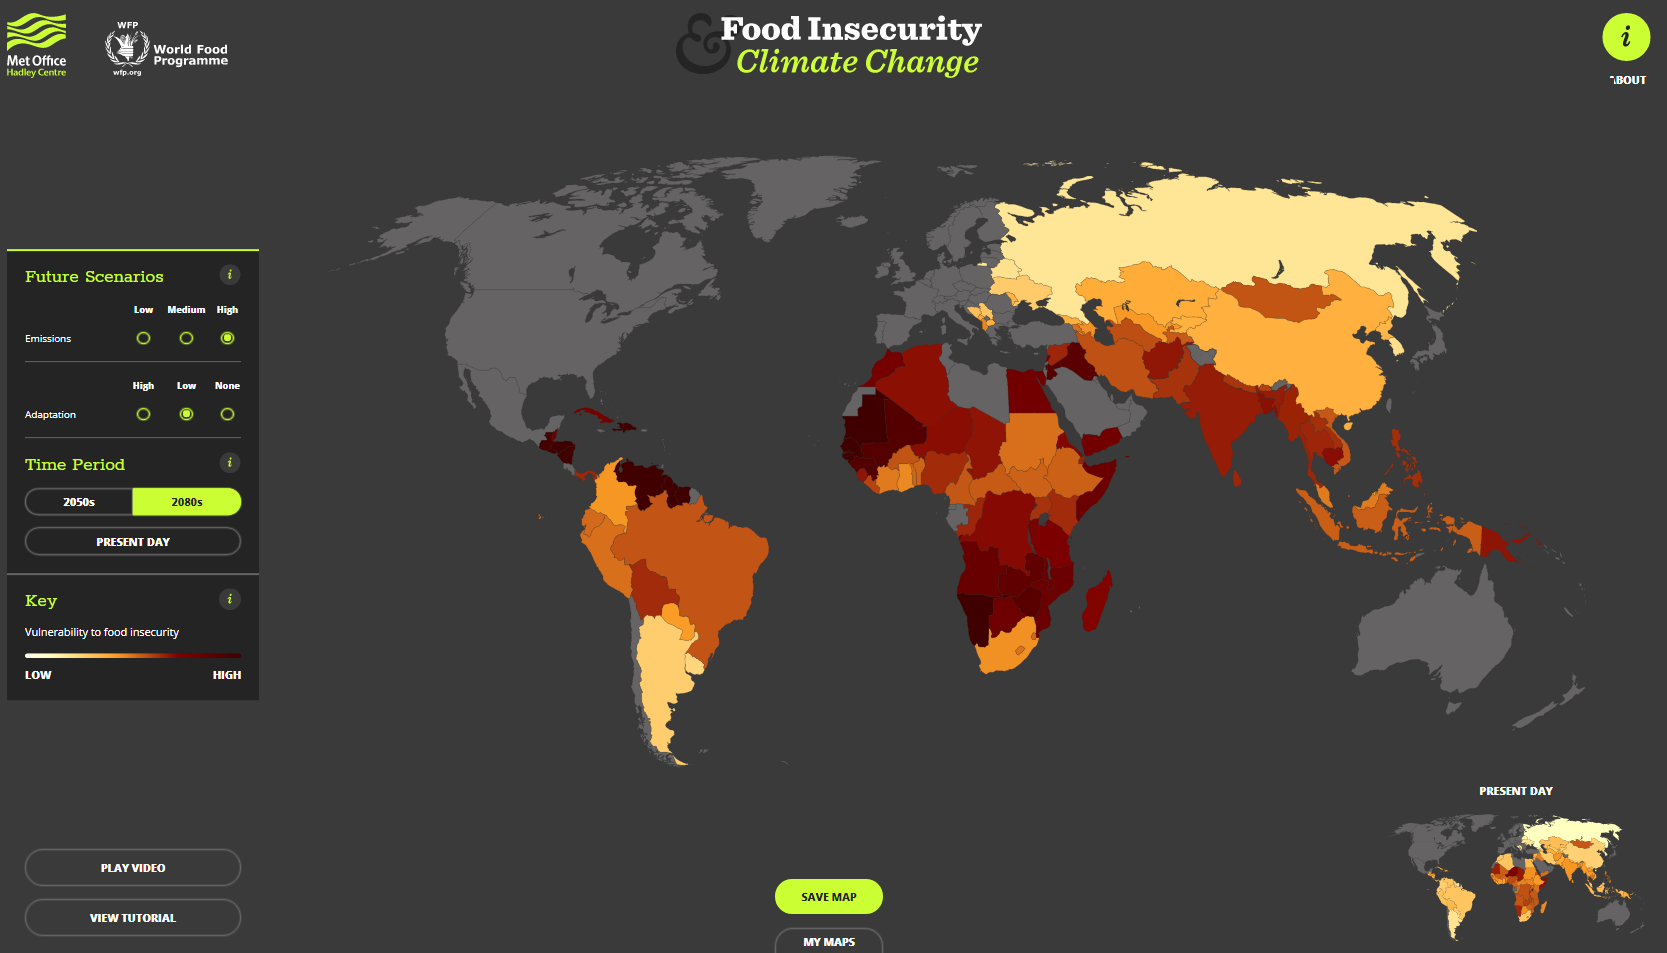
\includegraphics[width=\textwidth]{figures/metOffice.png}}
	\caption[MET OFFICE FOOD INSECURITY \& CLIMATE CHANGE WEBSITE]{Met Office Food Insecurity \& Climate Change website (www.metoffice.gov.uk/food-insecurity-index). The Met Office is the United Kingdom's national weather service. Their visualization shows a measure of how vulnerable a country's food security system is to the negative impacts of weather and climate \citep{metofficeCitation}. The darker red colors indicate a higher level of vulnerability. Future scenarios allow for predictions based on the options selected. The current display shows the vulnerability to food insecurity for the 2080s based on a scenario of high emissions and low adaptation levels.}
	\label{metOffice}
\end{figure}
Trade data can be visualized directly on the FAOSTAT website as seen in figure \ref{faostatViz}. This data visualization takes one country and displays the import or export trade links of a single trade good for that country. The visualization is done as a geographic choropleth representing the quantity or value of the imported or export good to another country. However, the visualization is ineffective as it only displays a single country's import or export contribution. It does not take into consideration the food trade network as a whole and does not allow for any interactions. These limitations again preclude any use for analyzing the effects of a change to the food trade network.\par
\begin{figure}[htb]
	\center{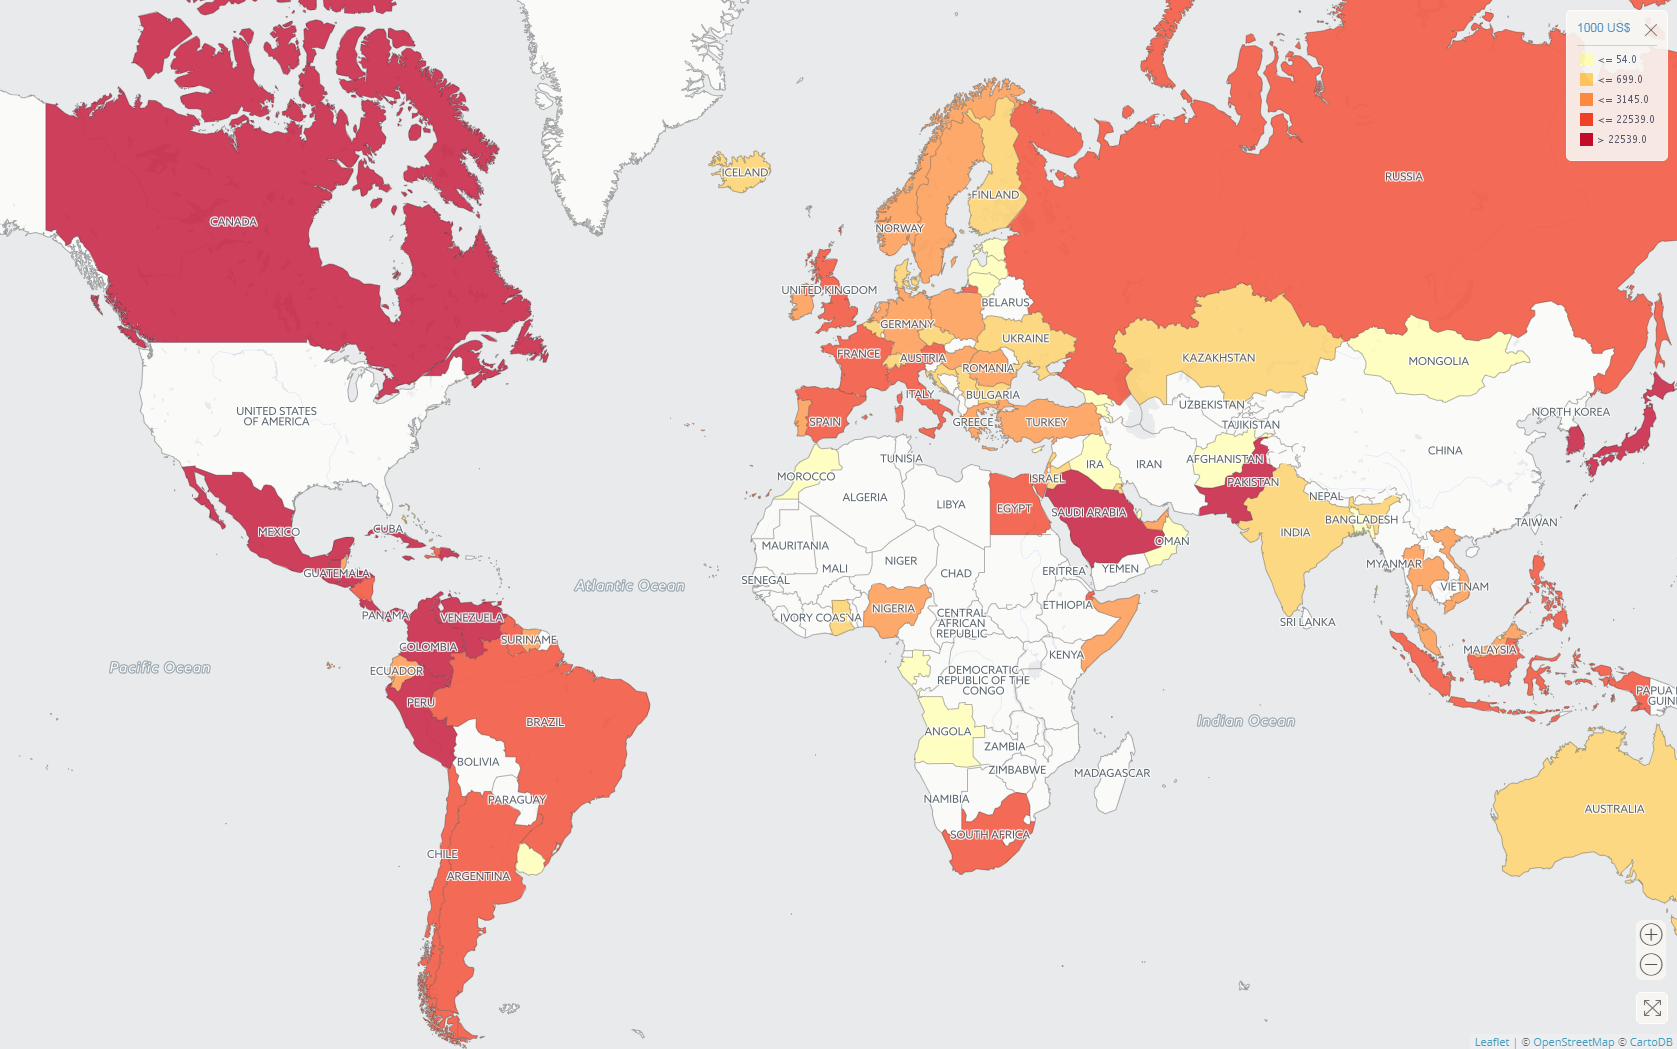
\includegraphics[width=\textwidth]{figures/faostatViz.png}}
	\caption[FAOSTAT DATA VISUALIZATION WEBSITE]{FAOSTAT data visualization website (www.fao.org/faostat/en/\#data/TM/visualize). The FAOSTAT is Food and Agriculture Organization of the United Nations Statistics Division. Their system shows the value of import or export trade links to or from the selected country for the given time period in a choropleth. The current display shows the dollar value of corn exported by the United States in the year 2013. The darker red the color a country is colored, the more the United States exported to that country. }
	\label{faostatViz}
\end{figure}

\section{Trade Networks and Food Security}
The increase of globalization has led to a marked decrease in the proportion of hungry people globally \citep{godfray2010food}. The international food trade network is used to feed people that were traditionally reliant on domestic production. Given that countries are becoming increasingly more import dependent \citep{d2014feeding}, the effects of disruptions to the food trade network are magnified. \cite{kali2007architecture} suggest that a network approach considering the cascading of shocks will be invaluable.\par
\cite{headey2011rethinking} highlights recent food crises and associates them to disruptions in the international food trade network due to surges in cereal prices. The cereal price surge in 2007 and 2008 is explored with an emphasis on how four staple good markets were negatively affected, leading to food security issues. Export restrictions and droughts were a major player in the volatility of the international food trade network at the time. According to \citep{brobakk2011increasing}, uncertainty in markets can lead to export bans which can lead to food insecurity. These works help provide understanding of the interaction between the trade network and food insecurity.\par
The food trade network can also be a tool to help deal with food security issues. Most of the global population is a resident of a net food importing country and so not self-sufficient, concluding that the world has moved from food insufficiency to an increasing food trade dependency \citep{porkka2013food}. This is especially true in the Middle East. The majority of Arabic countries import more than 50\% of their caloric intake \citep{faostat}. Suppliers are limited, with five exporters (Argentina, Australia, Canada, the European Union and the United States) accounting for almost three-quarters of the world's traded staple crops \citep{faostat}. \cite{d2016teleconnected} classifies countries vulnerability based on their level of caloric trade dependency. High dependency on a single staple crop for supply of calories and a high dependency on imports indicates a higher risk. This model of risk is used as the basis for the vulnerability index in this thesis.\par
Identified vulnerable countries also receive their imports from just a few dominant producing countries. \cite{silberglitt2015critical} explains the concern of two-tier pricing involved in concentrations of producers. Producers are able to influence the pricing on the market by enforcing export restrictions or bans, resulting in preferential domestic supplies. This has the potential of exacerbating the effects of a supply-side shock, which can be devastating to the entire food trade network. Exposure to non-domestic supply shocks is a trade-off to an increasingly globalized food trade network. According to \cite{gephart2016vulnerability}, exposure to this risk can be reduced by a diverse trade portfolio. These supply shocks are one representation of the cascading effects of a climate event.\par
An example of a supply shock by a major exporter is reviewed in \cite{fellmann2014harvest}. Russia, Ukraine and Kazakhstan temporarily placed export bans on wheat following poor harvest due to drought. This shows that shocks affecting more network-central countries are more likely to be transferred to other areas of the network. Net grain importing countries are at a major risk when diverse import trade portfolios are not present. This previous work provides the basis for my first case study.\par
The value of a link in the food trade network can be represented in many fashions. \cite{macdonald2015rethinking} suggest that in the modern era of globalization it may be more beneficial to think of a product's values using a resource metric such as cropland area. Monetary value can change with a number of factors and is so discouraged. Another useful metric we discovered may be calories or virtual water. Expanding on the concept of virtual water \cite{hoekstra2005globalisation} quantifies the calculations of water demand for specific crops. Virtual water balances are defined as the difference of gross virtual water imports and exports. Developed countries tend to have a more stable virtual water balance. Knowledge of the national virtual water balance is important in policy development because water scarcity is a driver of international food trade. \cite{konar2011water} explores the virtual water trade network as a amalgamation of the international food trade network. The topic provides a framework for use of water trade as the network model. Network graph statistics are produced for the virtual water representation of the international food trade network. Dominant countries are highly connected and are identified as hubs which connect to the large number of small trade-volume countries. \cite{hoekstra2012water} introduces water footprints and illustrates the global dimension of water consumption and pollution by showing that several countries heavily rely on foreign water resources. Many countries have significant impacts on water consumption and pollution elsewhere. Policies in this context translate to food security concerns and water footprints should be understood for development of these policies. This also solidifies the relationship between climate events, which generally affect water availability, and the food trade network. Because of increased globalization climate events are no longer localized and these regional events may have global effects on food security \citep{sternberg2012chinese}, validating the need for this second-order effect model.\par
Related work in the area of the international food trade network provides the preliminary domain-knowledge required for the effective development of a related visual analytic system. With understanding of the interactions and consequences of perturbations to the food trade network I was able to more effectively model the food trade network's cascaded effects. The literature reviewed here allowed for the connection between food insecurity vulnerability and the food trade network.\par







\section{Network Graphs}
To accurately model cascading effects we need to understand the topology of the international food trade network when represented as a node-edge graph. \cite{serrano2003topology} states the world trade network has become a self-organized complex system that must be considered in its entirety.\par
The international food trade network is essentially a very dense network graph and can be modeled as $G=(V,E,W,T)$. $V$ is the set of vertices, represented by all the countries involved in the food trade network. $E$ is the set of trade links, defined $E_n=\lbrace V_i, V_j, t \rbrace$. Direction is indicated with the importing country represented by $V_i \in V$ and the exporting country, $V_j \in V$. $T$ is the set of all trade goods. The good represented by an edge is $t \in T$. The weight of the edge is the defined as the function $w_{i,j,t}$. The weight function is the dollar value of the trade link of the specified good from country $j$ to $i$. The number of nodes is limited to the number of countries involved but the number of edges is extraordinary due to the large number of goods being traded and the number of unique trade partners.\par
Subgraphs are pieces of more complex networks and specifically three node subgraphs are labeled as triads. \cite{milo2002network} classifies these subgraphs occurring a significantly higher rates than expected as motifs. There are examples of motifs found in biological \citep{shen2002network}, technological \citep{milo2002network} and agricultural \citep{shutters2012agricultural} networks. The recurrence of these motifs show patterns that occur much more frequently in real networks than in randomized networks. This indicates that a structure exists which can be classified. A number of different classifications are presented and motif frequencies are examined for those distinct types. These network motifs are discovered here and also in \cite{grochow2007network}. This introduces a novel approach for motif discovery that utilizes a method for searching for a single network motif as opposed to enumerating subgraphs. It also takes advantage of symmetry of motifs to reduce the number of iterations. \cite{stouffer2012evolutionary} contains information on the different unique motif positions. This provides the reference when identifying the positions as well as the triad numerical classification. There are between one and three different unique motif positions depending on the type and thirty different unique positions over the thirteen different triads. The number and type of motifs in a network are important characteristics that directly affect stability of the network. The usefulness of using a reciprocal model for determination of the type of triad is confirmed in \cite{squartini2012triadic}. Models should take into account not only in the in and out degrees of the motifs but also the reciprocity of the links. With this representation the model can replicate the triadic structure. This suggests the dyadic structure of the network is information rich. \cite{zhou2016structure} employs a model that uses country behavior in the local triadic environment to account for the formation of such network structure. Different network graphs are created based on a country's top one or two trading partners. These truncated network graphs are shown to extract the more important information of the network. In this system these classifications of subgraphs are used to construct the triads.\par
Triad significance profiles (TSP) are an area of emerging research where the prevalence of certain triads is compared to normal distributions. \cite{winkler2013motifs} produces generative models that would create network graphs based on these triadic z-score profiles. \cite{shutters2012agricultural} lays the groundwork for association of triad significance profiles in the international food trade network to economic health. There are similarities of agricultural trade network with known triad significance profile of human social networks and biological information processing networks to a lesser degree. Superfamilies of existing networks are compared against the international food trade network and a distinct superfamily for the food trade network is identified. My framework visualizes these TSP for potential association to food trade network health.\par
Other related works focus on the international food trade network's specific network graph statistics \cite{fagiolo2010evolution} and topology \citep{serrano2003topology}. The density of the network graph as indicated by \cite{schiavo2010international} shows that there is a high level of clustering and that the topology of the international trade network is indeed important. Three data points for nodes are defined; node degree (the number of links maintained by each node), average nearest neighbor degree (the correlation between the degree of a node and the average degree of its partners) and clustering coefficient (the percentage of pairs of a node's partners that are connected among themselves). Importance should be given to the distribution of trade links across all trade partners. \cite{kali2007architecture} explains that a country's position in the network has substantial implications for quantifying economic growth. The majority of countries involved in the trade network are characterized by weak links, with a small number of countries exhibiting strong relationships indicating a core-periphery structure. The clustering coefficient is high in the international food trade network and has a high level of centralization, implying a hierarchical structure as suggested in other research (\cite{zhou2016structure}, \cite{garlaschelli2005structure}). \cite{zhou2016structure} constructs the network based on the top trade links and indicates there is indeed a hierarchy. \citep{ravasz2003hierarchical} and \citep{zhou2016structure} show that real networks are not randomized, but follow a pattern of organization related to hierarchy. At higher levels of trade, the network is considered scale-free; there is no typical country in terms of number of trading partners. The properties of scale-free networks are examined in \cite{li2005towards}. The power law degree distributions of the international food trade network align with these observations.\par
As the international food trade network was modeled as a network graph, the literature reviewed here allowed for an effective understanding of the underlying construction. The dependencies in the food trade network are related to the topology of the network graph. Although TSP analysis was passed in favor of a cascading effect model the foundation for future work is established with the related work here.\par


\section{Visual Analytics}
Visual analytics has become the preferred tool for domain-experts exploring large data sets. It is defined by \cite{cook2005illuminating} as ``analytical reasoning facilitated by interactive visual interfaces.'' \cite{shneiderman1996eyes} introduces the well-known information seeking mantra: overview first, zoom and filter, then details-on-demand. Visual analytics, per \cite{keim2006challenges}, extends this mantra to include the combination of data analysis and interactive visual interfaces: ``analyze first, show the important, zoom/filter/analyze further and details on demand.''\par
	\begin{figure}[htb]
		\center{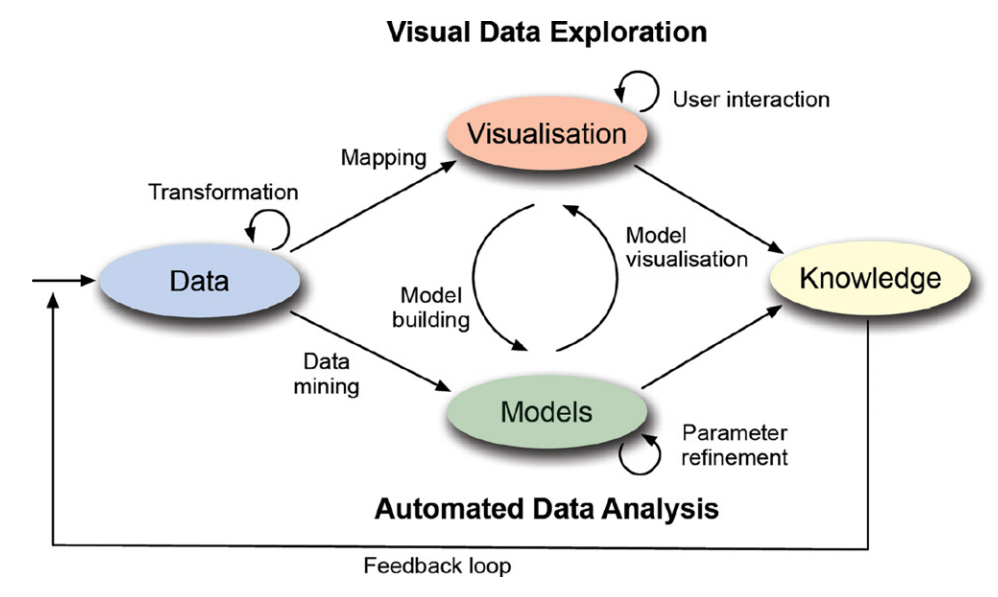
\includegraphics[width=\textwidth]{figures/keim.png}}
		\caption[VISUAL ANALYTICS FRAMEWORK]{Visual Analytics Framework, (\cite{keim2008visual}, \cite{kohlhammer2011solving})}
		\label{keim}
	\end{figure}
\cite{keim2008visual} introduces the framework for visual analytics (Figure \ref{keim}). The framework captures the process of a typical sense-making session. First, data is transformed by filtering and models are built from the resultant data subset. Visual data exploration is then applied with interactive visualizations to analyze and explore the data. Automatic analysis is done at each iteration of a feedback loop to produce results. The feedback loop helps repeat this process until sufficient refinement of the results is achieved. This automated analysis techniques were used by this thesis to calculate vulnerability indices after each iteration of the feedback loop.\par
To build the visual analytics system, the first step is data analysis. Previous research (\cite{zhou2016structure}, \cite{shutters2012agricultural}, \cite{squartini2012triadic}) has provided some initial data analysis that is supplemented by our own resources. Triads are calculated, motif positions are generated and bilateral trade links are computed. Further analysis is accomplished by the user interaction and filtering of interesting data in the feedback loop.\par
The next step is analysis via interactions with the visualizations. In visual analytics involving graphs, \cite{sun2013survey} shows recent research has focused on the visual mapping aspect of the analytics systems over the model-based analysis. Graph data is highly structured and is a possible reason for this paradigm.\par
Visualizing a network graph can be done in two primary ways: node-link diagrams and adjacency matrices. The most familiar visualization is the node-link diagram . \cite{ghoniem2004comparison} considers the two different representation and compares the readability of the two graphs. Although the international trade network starts out with a large number of nodes, when filtering is applied \citep{shneiderman1996eyes} it has a limited number of nodes. Therefore when choosing the appropriate visualization I consider it a small graph, and node-link diagrams are more readable \citep{ghoniem2004comparison}.\par
Node placement is a consideration when network visualization is concerned. A common layout strategy is based on geographic representation \citep{shneiderman2006network}. This geographically representative positioning is used in both of the main visual representations. The linked multiple views of the familiar world map (choropleth) and the network visualization allow for a greater understanding \citep{rodgers2005graph} and allow for mental mapping \citep{eades1991preserving}.\par
When visualizing a network minimizing edge crossing is the most important aesthetic consideration \citep{purchase1997aesthetic} for improving human comprehension. A number of different algorithms for graph visualization were reviewed (\cite{herman2000graph}, \cite{dunne2013motif}, \cite{holten2009force}) that help with this consideration. \cite{herman2000graph} overviews a number of basic graph layout algorithms in the context of information visualization. \cite{dunne2013motif} offers a technique to simplify highly clustered network graphs by aggregating subnetworks. Simplifying the drawing of certain types of motifs can greatly increase readability in dense network graphs. \cite{holten2009force} shows another example of a technique aimed at simplifying complex network graphs. This is achieved by bundling of similarly drawn edges and subsequent splitting of the edges closer to the termination node. Ultimately these algorithms were removed from consideration in favor of mental mapping \citep{eades1991preserving} and interpretability \citep{keim2008visual}. Nodes were positioned approximately geographic to aid in the establishment of this mental map. The minimization of edge crossing is accomplished interactively by dragging of nodes after a simulation baseline is established.\par
The parameters for the algorithms are usually considered in multiple solutions before results are achieved \citep{hund2016visual}. In this system the reasoning is done by the human analyst \citep{andrienko2011challenging}, and the interaction allows for the parameters of the algorithms to be manipulated by the users.\par
Knowledge in this field was pertinent to the development of effective human computer interaction techniques used in this system. The visual analytic paradigm providing for the feedback loop was implemented to allow for analysis of the effects of a simulated climate event.\par
The work reviewed here provides the framework for my visual analytic system. I build the framework on the principles defined in the visual analytics mantra \citep{keim2006challenges}. The representation of the network graph as a node-link diagram instead of an adjacency matrix was based on the suggestions of previous research included in this section. The visual design was also inspired by the mental mapping paradigm.\par
%\chapter{THE INTERNATIONAL FOOD TRADE NETWORK}
\label{foodTradeNetworkChapter}
\section{Data Source}
\section{Description}
The international food trade network is made up of a large number of trade links. Each link is defined as a trade year, an exporting country, an importing country, the trade item, the trade quantity (usually in tons), and the trade value. For the purposes of the dashboard the data was scoped to the trade value and the trade quantity was removed. 

\section{Structure}

\section{Trade Dependencies}

%\chapter{NETWORK STRUCTURE AND ANALYSIS}
\label{networkAnalysisChapter}
\section{Triadic Motifs}
The actual distributions are quite different than randomized distributions and thus indicate a particular structure \citep{milo2002network}. These structures may vary depending on the context but there are striking similarities between the motif distribution in these agricultural trade networks and other well known network graphs such as the human social networks and biological informational processing networks \citep{shutters2012agricultural}. The network graph is also self-organizing, with distribution trending towards a normal value \citep{squartini2012triadic}.\par


%\chapter{EFFECTIVE VISUALIZATIONS}
\label{effectiveVisualizationsChapter}
\section{Visual Information Seeking Mantra}
The visual information seeking mantra, defined by \cite{shneiderman1996eyes}, indicates that it is important to follow the steps overview first, zoom and filter, then details-on-demand when starting any information visualization. The dashboard was created with this in mind.
\subsection{Overview}
To achieve this aspect of the the dashboard starts by presenting all the data. An overview of the international food trade network, and particularly its complexity, can be seen immediately in the network graph (figure \ref{networkGraph}). The zoomed out view of both the network and cartographic maps allow for browsing the entirety of the collection.
\subsection{Zoom}
Zooming is done in both the cartographic and network visualizations. In the cartographic section it allows the user to see impacts to individual countries as in figure \ref{zoomed}. In the network graph section zooming facilitates exploration of geographically dense areas, such as Europe, (figure \ref{zoomedNetwork}).
	\begin{figure}[htb]
		\center{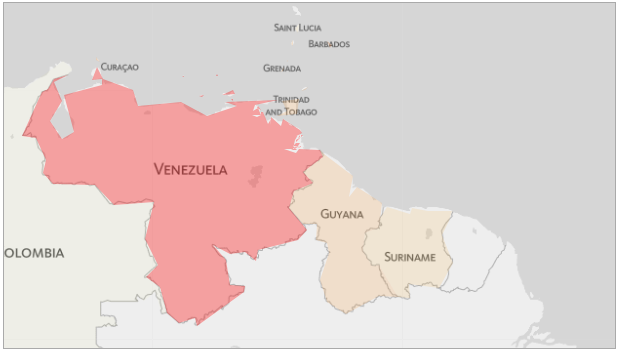
\includegraphics[width=\textwidth]{figures/zoomed.png}}
		\caption{A zoomed in view of the cartographic map.}
		\label{zoomed}
	\end{figure}
	\begin{figure}[htb]
		\center{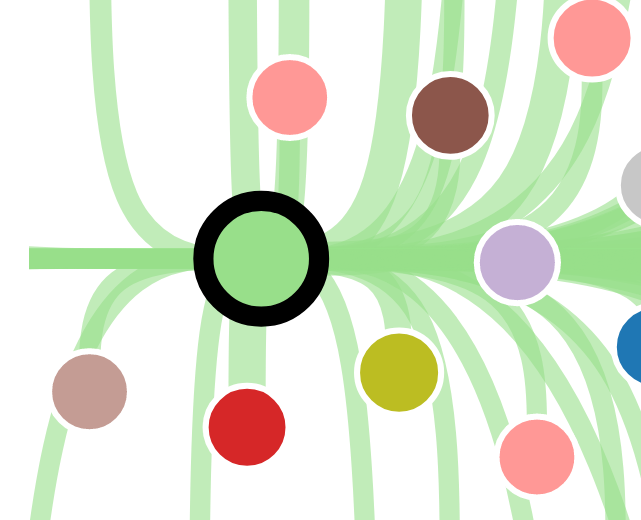
\includegraphics[width=\textwidth]{figures/zoomedNetwork.png}}
		\caption{A zoomed in view of the network graph.}
		\label{zoomedNetwork}
	\end{figure}
\subsection{Filter}
The tool allows filtering on a number of different parameters. The user can filter the trade good they wish to explore, the year they wish to examine, or the impacted country.
\subsection{Details on Demand}
Details are provided as tooltips in most sections of the dashboard. Hovering over the histograms show trade links that make up that particular bin. These can be used to identify susceptible trade links and prompt further filtering. A country's economic contribution in the network of the selected trade good can be seen by hovering over the country.
\section{Visual Analytics Dashboard}
\cite{keim2008visual} defines visual analytics as combining automated analysis techniques with interactive visualizations for an effective understanding, reasoning and decision making on the basis of very large and complex data sets.\par
The inclusion of prediction choropleth on the cartographic map helps transform the information visualization into a visual analytics tool. By aiding the user in making correlations we allow for that decision support. Allowing for filtering helps maintain the feedback loop \citep{keim2008visual} in which the user can make a decision.

%\chapter{DATA}
\label{dataChapter}
\section{Data Source}
The data were sourced from the United Nations FAOSTAT. A snapshot including up to 2013 data, was loaded onto the Visual Analytics and Data Exploration Research Lab at Arizona State University (VADER) database. Further processing was done to calculate the triadic motifs. Over 172 million individual triadic motifs were calculated from 8 million trade links.\par
\section{Simulation Formulas and Assumptions}
In the simulation of climate singularities the trade link value for all the selected country's export links is reduced. For instance, if we simulate a 10\% reduction in wheat exports from a country, every export trade link is reduced by 10\%. The reduction percentage is a reduction of export links and not a reduction of production. This is an important assumption because if we assumed a production reduction it could potential decrease the export trade links by a larger amount than the actual production reduction for the country to maintain its own stores of the trade good. It should also be said that the export links will all be reduced regardless of outside influences. There is no favoritism in decision making of the reduction of exports; that is, there is an equal reduction in goods to all trading partners.
\chapter{SYSTEM}
\label{systemChapter}
The goal of the proposed visual analytic system is to enable analysts to simulate the first- and second-order effects of climate events to the food trade network. Identification of the effects, along with potentially vulnerable countries, can be used by policy makers and international aid managers. For instance, in the event of a drought in Argentina, analysts would be able to use the framework to determine which countries would likely be impacted the most. They could then advise international aid managers to begin staging supplies near the predicted areas.\par
\section{Data, Assumptions, and Formulas}
\label{daf}
	The Food and Agriculture Organization (FAO) of the United Nations (UN) Statistics Division maintains the Food and Agriculture Organization Corporate Statistical Database (FAOSTAT). This database provides free access to food and agriculture data for over 245 countries and territories and covers all FAO regional groupings from 1961 to the most recent year available (\cite{faostat}).\par
	The data in this thesis is a snapshot from the FAOSTAT database containing trade link data for the years 1986 through 2013. The FAOSTAT database contains a reporting country, a partner country, the type (i.e. import or export), the trade year, the trade good and dollar value. A country will report the value of a particular good it imported for that year from the partner country. That partner country also reports the exporting value. Since these two reports are not always the same, as seen in Table \ref{faotableLinks}, some preprocessing is required.\par
	\begin{center}
		\begin{table}[htb]
			\begin{tabular*}{\textwidth}{@{\extracolsep{\fill}}|l|l|l|l|l|l|}
				\hline
				Trade Year&Reporter&Partner&Type&Item&Value\\
				\hline
				2011&USA&Japan&Maize&Export&{\$3,831,683,000}\\ \hline
				2011&Japan&USA&Maize&Import&{\$4,818,714,000}\\ \hline
			\end{tabular*}
			\caption[SAMPLE FAOSTAT DATA]{Sample FAOSTAT data}
			\label{faotableLinks}
		\end{table}
	\end{center}\par
	Since the FAOSTAT database contains two sets of data, the importing country's reported data and the exporting country's reported data, preprocessing was done to merge the two reported values. The processed trade links are then defined by the exporting country, the importing country, the trade year, the trade good and the dollar value of the trade link. Some example links are shown in Table \ref{tableLinks}. Bilateral trade associations and triad constructions were calculated and stored in our database.\par
	\begin{center}
		\begin{table}[htb]
			\begin{tabular*}{\textwidth}{@{\extracolsep{\fill}}| l | l | l | l | l |}
				\hline
				Trade Year & Exporter & Importer & Item & Value \\
				\hline
				2011 & USA & Japan & Maize & {\$4,325,199,000} \\ \hline
				2011 & Poland & Sweden & Molasses & {\$2,648,000} \\ \hline
				2011 & Afghanistan & Australia & Almonds shelled & {\$13,000} \\ \hline
			\end{tabular*}
			\caption[SAMPLE TRADE LINKS COMPRISING THE INTERNATIONAL FOOD TRADE NETWORK]{Sample trade links comprising the international food trade network}
			\label{tableLinks}
		\end{table}
	\end{center}\par
	To model the cascading effects of a climate event a simulation engine was created. In construction of the simulation engine we made the following assumptions. First, for the simulation of a climate event, the trade link value for all the selected country's export links is reduced. For instance, if a 10\% reduction in wheat exports is simulated from a country, every export trade link is reduced by 10\%. Second, the reduction percentage is a reduction of export links and not a reduction of production. This is important because if a production reduction is assumed it could potentially decrease the export trade links by a larger amount than the specified reduction for the country to maintain its own stores of the trade good. Another benefit is that we are able to model indirect export reductions, such as export restrictions. Third, the export links will all be reduced regardless of outside influences. There is no favoritism in the decision making of which export trade links to reduce; that is, there is an equal reduction in trade goods to all trading partners. Lastly, the reduction in imports to a country is then extrapolated to its own export trade links. The country is calculated to lose that value of goods and will first reduce its own exports to mitigate the loss of imports. Such assumptions pose the risk of an overly simplistic export reduction formula which may not be realistic, however we believe that it does offer a good starting point.\par
	The vulnerability index to a country is then defined as 
	\begin{equation} \label{vulnerability}
		v=\frac{\sum _I - \sum _{I_\Delta}}{\sum _I + \sum _E}
	\end{equation}
	where $\sum _I$ is the sum of the country's import trade links dollar values before the simulation reduction, $\sum _{I_\Delta}$ is the sum of all of the country's import trade link dollar values after the simulation reduction and $\sum _E$ is the sum of all of the country's export trade link dollar values before the simulation reduction. Note that denominator is the sum of both import and export trade link dollar values. Again, we make the assumption that a country would reduce its exports to overcome the loss of imports.The range of values is 0 to 1 and a higher number indicates a higher vulnerability. If a country does not suffer any import reduction, that is $\sum _{I_\Delta}=\sum _I$, then the vulnerability index will be 0: $v=0$. If a country loses its entire import portfolio, that is $\sum _{I_\Delta}=0$, the vulnerability index is then a function of the value of its ratio of its imports and exports: $\frac{\sum _I}{\sum _I + \sum _E}$. If that country does not have any export links, that is $\sum _{E}=0$, then the vulnerability index is a function of the value of lost imports: $\frac{\sum _I - \sum _{I_\Delta}}{\sum _I}$. If a country does not have any export links and loses its entire import portfolio, that is $\sum _{E}=0$ \& $\sum _{I_\Delta}=0$, then the vulnerability index will be 1: $v=1$.\par
	Another index used in the system is import dependence, defined as 
	\begin{equation} \label{importRatio}
	d_l=\frac{l}{\sum _I + \sum _E}
	\end{equation}
	where $l$ is the dollar value of the trade link and $\sum _I$ is the sum of the all of the country's import trade link dollar values and $\sum _E$ is the sum of the all of the country's export trade link dollar values. The higher the number the higher the import dependency of the trade link. Note that denominator is the sum of both import and export trade links. Again, we make the assumption that a country would reduce its exports to overcome the loss of imports.
	\section{System Architecture}
		The proposed visual analytics system is a web-based system consisting of a front-end website for user display and interaction and a back-end system for data retrieval. The system is accessible from a modern web browser and was developed with an HTML front-end utilizing JavaScript for advanced features. The core of the visualization was created by an open-source JavaScript library called Data-Driven Documents (D3), \citep{d3}. This is a JavaScript library providing many mechanisms for manipulating document object model (DOM) elements based on data. A powerful concept which was utilized extensively was selections. This allows attribution of an array of data to an element, usually a DIV. Then child nodes are created, updated, and destroyed based on changes to the array. This mechanism allowed a extremely large dataset to be held in memory. The benefits of this are two-fold; efficient manipulation of the dataset resulting in responsive visualizations and reducing the need for numerous database calls limiting the effect of network latency.\par
		Connecting the front-end to the back-end are RESTful APIs. The APIs exist on the back-end web servers to connect to a database and provide the data to the front-end. These APIs were written in Java and utilize a mechanism to execute simple transactional-SQL queries. The data is then returned in a D3 friendly arrayed JavaScript Object Notation (JSON) formatted object for processing in the front-end.\par
	\section{Visual Analytics Framework}
		A diagram of the visual analytic framework is shown in Figure \ref{architecture}. The three parts of the system are the data, the model and the visualization. In my system the data is the database and supplemental data as described in Section \ref{daf}. The model part of the system is accomplished by modeling the trade links as a network graph and calculation of vulnerability indices, triad z-scores and import dependencies. These calculations are described in more detail in the following sections. The visualization graphically represents the data and models to allow for analysts to visually detect patterns. The feedback loop is made up of the action and finding boxes on the right side of Figure \ref{architecture}.\par
		My framework allows for a domain expert to simulate a climate event to explore the first- and second-order effects to the international food trade network and identify any potentially vulnerable countries. After a subset of data is selected, a simulation is modeled and the visualization displays the effects. Further filtering and interactions, such as panning and zooming, in the feedback loop allow for enhanced pattern recognition.\par
		\begin{figure}[htb]
			\center{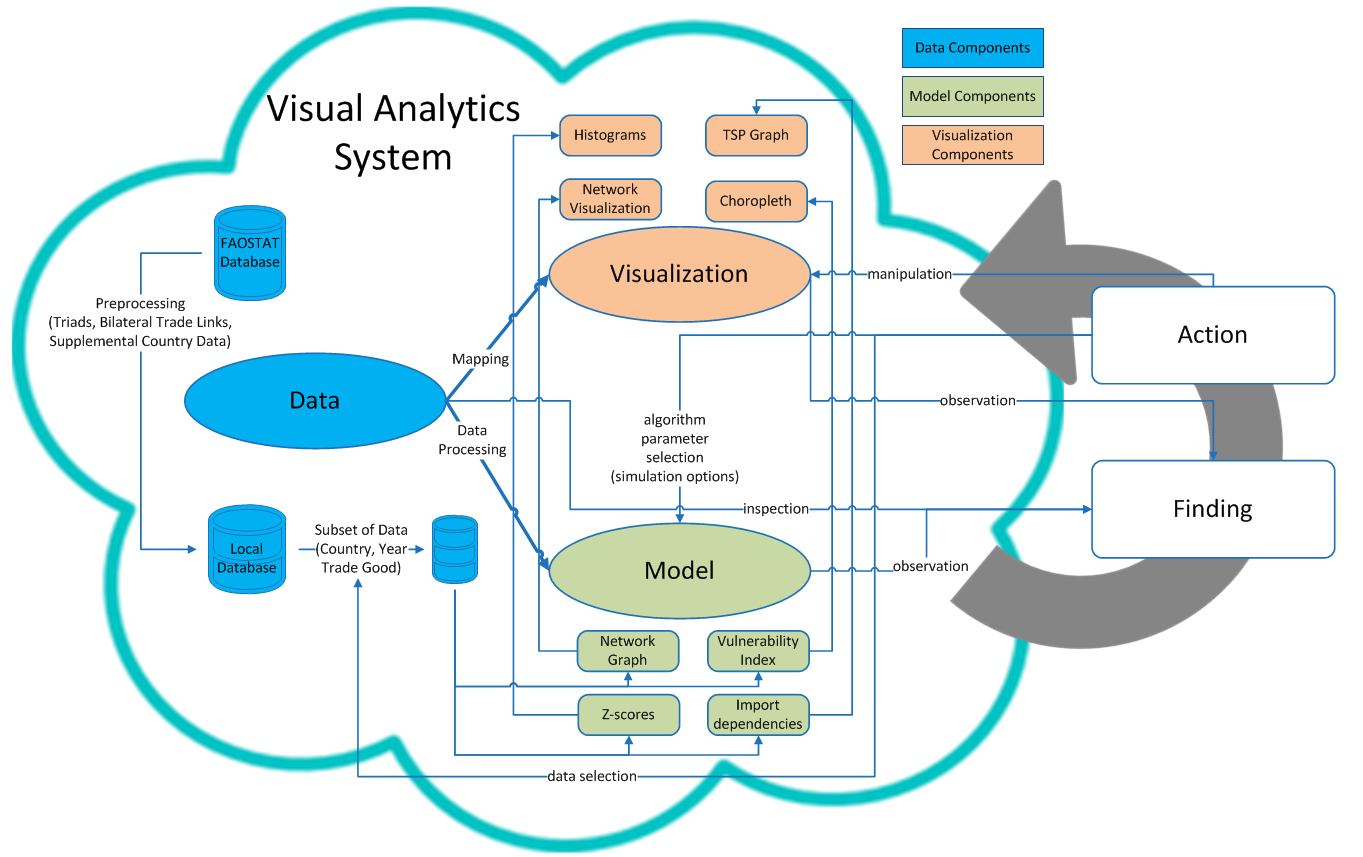
\includegraphics[width=\textwidth]{figures/va_system.png}}
			\caption[VISUAL ANALYTICS SYSTEM DIAGRAM]{Visual Analytics System diagram, (motivated by \cite{sacha2014knowledge})}
			\label{architecture}
		\end{figure}
		The main visualization of the visual analytic system is a dashboard (Figure \ref{dashboardSections}). In the top left part of the dashboard a combo box exists so the user may select the year to analyze. The rest of dashboard is composed of 5 distinct sections as seen in Figure \ref{dashboardSections}. The histogram charts in Figure \ref{dashboardSections}-1 shows the distribution of trade links based on the import dependency for four staple crops, with the most opaque indicating the currently selected crop. Figure \ref{dashboardSections}-2 shows the network graph, a visual representation of the food trade network, and all of the import and export trade links of the currently selected crop. Figure \ref{dashboardSections}-3 is the choropleth map which visualizes the impacts of the simulated climate event from Figure \ref{dashboardSections}-5. Both the network graph and choropleth map allow for a user to select a country for the simulation by clicking on the node in the graph or country on the map. The selected country is then given a dark border in both views as seen in Figures \ref{networkGraph} and \ref{map}. Figure \ref{dashboardSections}-4 shows the normal triad significance profile (TSP) graph based on four staple crops for the year 2013 overlayed with the TSP graph of the currently selected data subset. Figure \ref{dashboardSections}-5 shows the parameters for the climate event simulation engine. In each of the sections moving the mouse over pertinent parts of the visualizations displays a tooltip for displaying detailed information, as in Figure \ref{tooltip}. This tooltip displays the trade link data from a link of the 2013 wheat network graph. In 2013 Egypt imported \$576 million dollars which accounted for 23\% of total Egyptian wheat imports and 11\% of the total Egyptian imports of four staple crops.\par
		\begin{figure}[htb]
			\center{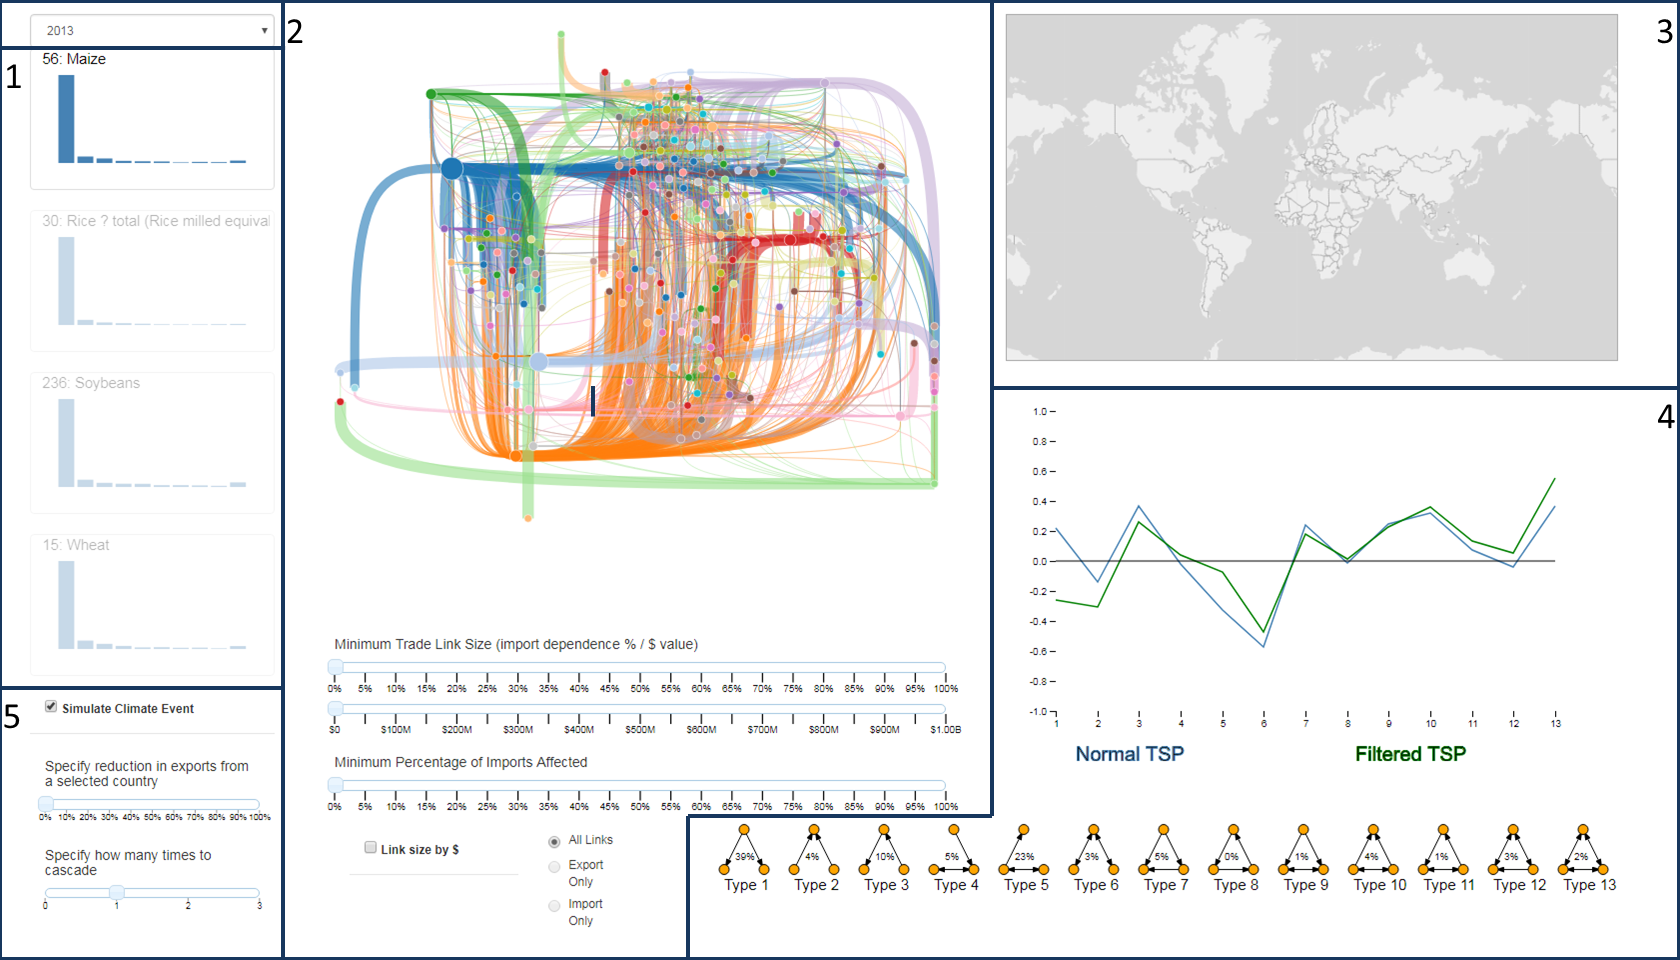
\includegraphics[width=\textwidth]{figures/sections.png}}
			\caption[SECTIONS OF THE DASHBOARD]{Sections of the dashboard. 1: Histograms of trade link import dependencies grouped by crop; 2: Network graph and filtering options; 3: A choropleth map visualizing the impacts of a simulated climate event; 4: Triad significance profile graph; 5: Climate event simulation engine parameters.}
			\label{dashboardSections}
		\end{figure}
		\begin{figure}[htb]
			\center{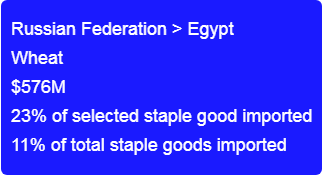
\includegraphics[width=150px]{figures/tooltip.png}}
			\caption[TOOLTIP OF A LINK IN THE NETWORK GRAPH]{A tooltip is displayed when the user moves their mouse over pertinent parts of the visualizations. In this example a tooltip displays the trade link data from a link of the 2013 wheat network graph. The tooltip shows the trade link values for that year. In 2013 Egypt imported \$576 million dollars which accounts for 23\% of Egyptian wheat imports and 11\% of the total Egyptian imports of four staple goods.}
			\label{tooltip}
		\end{figure}
		\subsection{Simulation Option (Figure \ref{dashboardSections}-5)}
			The simulation of climate events is the defining part of the system. This section allows for the parameters for the climate event simulation to be defined. The first checkbox in Figure \ref{dashboardSections}-5 indicates whether we want the simulation engine to run or not. The calculations for the simulation engine are time consuming so generally this is only checked after an interesting scenario is identified. The other controls in Figure \ref{dashboardSections}-5 only appear if the checkbox is checked and the choropleth map (Figure \ref{dashboardSections}-4) will only be colored in if a simulation is being ran.\par
			The slider in the next part of Figure \ref{dashboardSections}-5 indicates the total percentage of reduction in export links to simulate. The last slider in Figure \ref{dashboardSections}-5 indicates how many times the reduction should cascade down. Cascading zero times implies that only the selected country's direct importers are affected. Addition of the first cascade level will add the second-order effects of trade link disruption to the initial importer's export partners.\par
		\subsection{Histograms (Figures \ref{dashboardSections}-1, \ref{histogram})}
			The histogram charts in Figure \ref{dashboardSections}-1 show the distribution of trade links, based on import dependency (Equation \ref{importRatio}), for each of the four staple crops. The trade links are binned in increments of 10 percent. The first group is 0 to 10\%, the next 10 to 20\%, et cetera. The more opaque histogram chart indicates the currently selected good and clicking on any of the other histograms changes the selected good to the clicked chart. The y-axis of the histogram shows the quantity of trade links in each bin and the x-axis is the import dependency. For example, the furthest right bin represents the trade links which account for 90 to 100\% of the importing country's entire import portfolio of the trade good. The tooltips (example in Figure \ref{histogram}) in this section show the number of trade links in a bin and the top 10 trade links by dollar value. The trade link data shown on the tooltip is the exporting country, the importing country, the dollar value and the import dependency.\par
			\begin{figure}[htb]
				\center{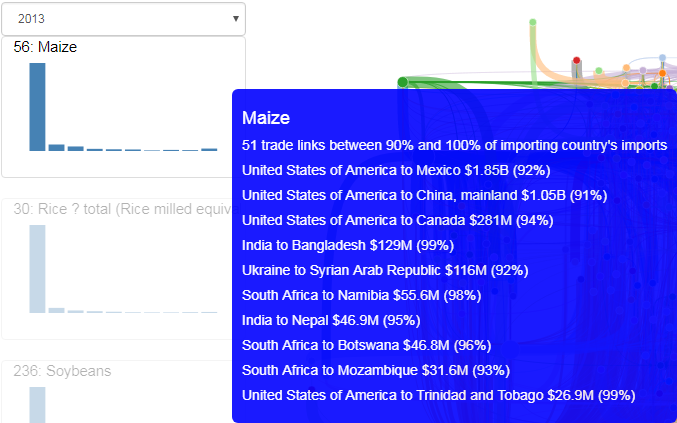
\includegraphics[width=\textwidth]{figures/histogram.png}}
				\caption[HISTOGRAM FOR CORN IN 2013]{A zoomed in view of the histogram for corn in 2013, with the tooltip showing information for the last bin. The trade links are binned into groups based on their percentage contribution to the importing country's total imports of that product. This can be used to quickly identify countries who have a large dependency on a singular trade link. The tooltip here shows that, in 2013, Mexico's import of corn was almost exclusively (92\%) from the United States at a trade value of \$1.85 billion.}
				\label{histogram}
			\end{figure}
			Generally, links in the left-most bins indicate more diversified imports and the right-most indicate imports that are made up of fewer trade links. This can be used to quickly identify countries that have a large dependency on a single trade link. As international food trade grows identification of reliance on imports is important to identification of vulnerability. Results from \cite{d2016teleconnected} and \cite{gephart2016vulnerability} suggest that diversification of trade partners reduce food security risks.\par
			An example is present in Figure \ref{histogram}. The presence of bins in the far right group in the histograms for corn (Figure \ref{histogram}) indicate that there is a large dependency for some countries on a single trade link. Mousing over the last bin and displaying the tooltip (Figure \ref{histogram}, tooltip) shows that in 2013 Mexico relied on the United States for about 92\% of its corn. Domain experts would be able to associate these types of links to potential areas of concern. If the importing country also exports we have the potential for the appreciation of cascading effects. By looking at bins that are in the at-risk group (furthest right in Figure \ref{histogram}) we can hover over the histogram and view the trade link information and corresponding import dependency. In this way the histograms can be used to select a country in the network graph or on the map as a starting point for exploration.\par
			With a country selected (e.g. Mexico) analysts would be able explore further questions such as: if a climate event affected the United States in a manner that was significant enough to prompt the United States to stop shipping corn to Mexico, even temporarily, what cascading effects do we see? Are any countries dependent on imports from Mexico? We are able to visualize these first- and second-order effects in the network graph and choropleth map.\par
		\subsection{Network graph (Figure \ref{networkGraph})}
			\begin{figure}[htb]
				\center{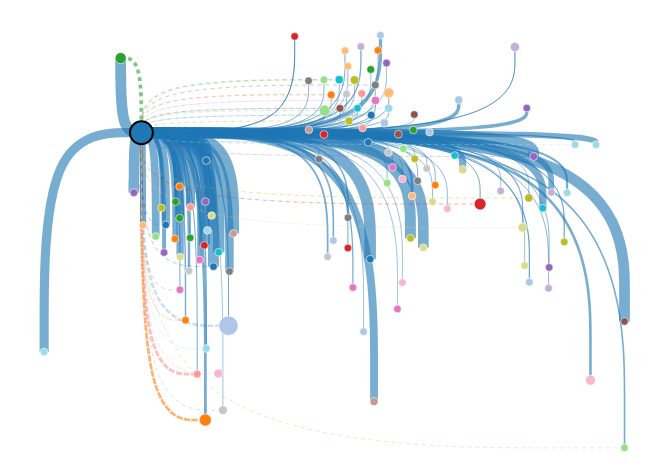
\includegraphics[width=\textwidth]{figures/networkGraph.png}}
				\caption[NETWORK GRAPH OF 2013 CORN IMPORTS AND EXPORTS FROM THE UNITED STATES]{A network graph showing all the corn that was imported or exported to the United States in the year 2013. The selected country is indicated by the dark outline of the node, in this case the United States (large blue dot on the left side). Node size is a function of the total GDP of the country. Solid lines indicate export trade links from the selected country if applicable. Dashed lines indicated import trade links to the selected country. Depending on the option selected the thickness of the trade links indicate the trade link's contribution to the importing country's total staple good imports or the trade link's dollar value.}
				\label{networkGraph}
			\end{figure}
			The international food trade market can naturally be represented by a weighted directed network graph as in Figure \ref{networkGraph}. Nodes of the graph are countries involved in trade and the edges are the trade links associated with the two countries. The node size is a function of the total GDP of the country. Node color is arbitrary but is constant for the life of the visualization. The nodes are positioned close to geographically correct with some perturbations for visual readability. Direction is indicated by color, the edge takes the color of the exporting country. For instance in figure \ref{networkGraph} the United States is blue and all export links from the United States are colored blue. Import links to the United States take the color of the exporting country, as. In the default view the weight of the link is the import dependency (Equation \ref{importRatio}) of the trade link. The weight of the link is indicated by the thickness of the line representing the edge. There is also an option (Figure \ref{networkGraphOptions}) to display the link size by dollar value. If no country is selected solid lines indicate both import and export trade links. If a country is selected its node will have a dark outline as in Figure \ref{networkGraph}. The large blue dot on the left side of the graph shows the selected country, in this case the United States. The edges are represented by solid lines, indicating export trade links from the selected country, and dashed lines, indicating import trade links to the selected country. If a climate event is being simulated alternating dashes and spaces indicate a link broken by the export reduction of the simulation. \par
			The three sliders in this section (Figure \ref{networkGraphOptions}) filter the network graph. The first slider in Figure \ref{networkGraphOptions} hides any trade links that have an import dependency of less than the selected value. This is used to potentially filter out insignificant trade links, e.g. accounting for 1\% of a country's total imports. The second slider filters out any trade links whose raw dollar value is not at least the selected value. Again this can be used to filter out insignificant links such as a trade link of \$1,000 dollars. The third slider is only visible in simulation mode and is used to filter out nodes whose total imports are affected by at least the slider's current value. This is useful for determining which countries are significant affected, including cascading effects, by the simulated climate event. The single checkbox will show the links weighted by dollar value instead of the import dependency (Equation \ref{importRatio}). The group of radio buttons will determine which type of links are shown. This is only available when a country is selected and not in simulation mode. There is also behavior for panning, zooming and node repositioning to facilitate interaction.\par
			\begin{figure}[htb]
				\center{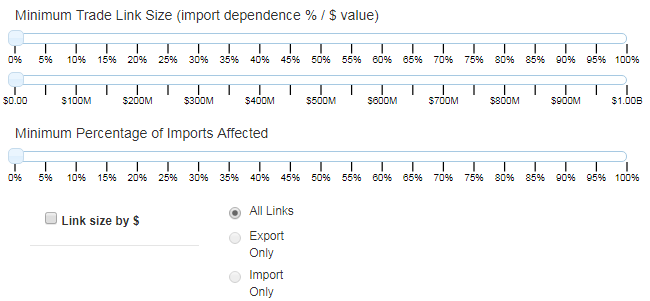
\includegraphics[width=\textwidth]{figures/networkGraphOptions.png}}
				\caption[OPTIONS FOR FILTERING AND DISPLAY OF THE NETWORK GRAPH]{Options for filtering and display of the network graph. The first slider hides any export trade links that contribute less than the selected value to the link's importing country's total import value of the trade good. The second slider filters out any trade links whose raw dollar value is not at least the selected value. The third slider is only visible in simulation mode and is used to filter out nodes whose imports are affected by at least the slider's current value. The single checkbox will show the links weighted by dollar value instead of the import dependency (Equation \ref{importRatio}). The group of radio buttons will determine which type of links are shown. This is only available when a country is selected and not in simulation mode.}
				\label{networkGraphOptions}
			\end{figure}
			The network graph is used to visualize trade links in the international food trade network. As risk is a function of import dependency the thickness of the link indicates the importance of that trade link to the importing country. Selecting a country here will filter the data to only include exports from and imports to the selected country. It is also required for any climate simulation as we need to define the country who will have their exports reduced.\par
			Continuing on the example from above, Mexico is the selected country and the trade links to and from Mexico are inspected. The tooltip for the link in the network graph (Figure \ref{mexicoMiddleMan}, tooltip) shows that although the trade link provides approximately 92\% of the corn imported to Mexico (from the histogram), it only accounts for about 37\% of the total imports of staple goods. This percentage can be used by a domain-expert to gauge the diversity of imports across the staple goods of the importing country to further evaluate the level of vulnerability. \par
			With a country selected analysts would also be able to see trade links upstream of a country. An example of this is in Figure \ref{mexicoMiddleMan}-2. Mexico is the selected country (purple) and the network graph is showing corn trade links for 2013, with trade links filtered by import dependencies of 25\% and dollar values of at least \$250 million. This has the effect of showing only the more significant trade links to and from Mexico. The large dashed line, indicating an import trade link, into Mexico shows that Mexico is highly dependent on the United States for a large portion of its corn (92\% from \ref{mexicoMiddleMan}-1, tooltip). The solid line, indicating an export link, out of Mexico shows that Venezuela is moderately dependent on Mexico for corn (29\% from \ref{mexicoMiddleMan}-2, tooltip). This would aid to identify countries that act as middle men, countries that also export the good they import. These countries' export partners are more susceptible to cascading effects due to climate events affecting their supply partner. This is especially true if the middle man has a high dependency on a single trade link as in this example of Mexico and the United States.\par
			\begin{figure}[htb]
				\center{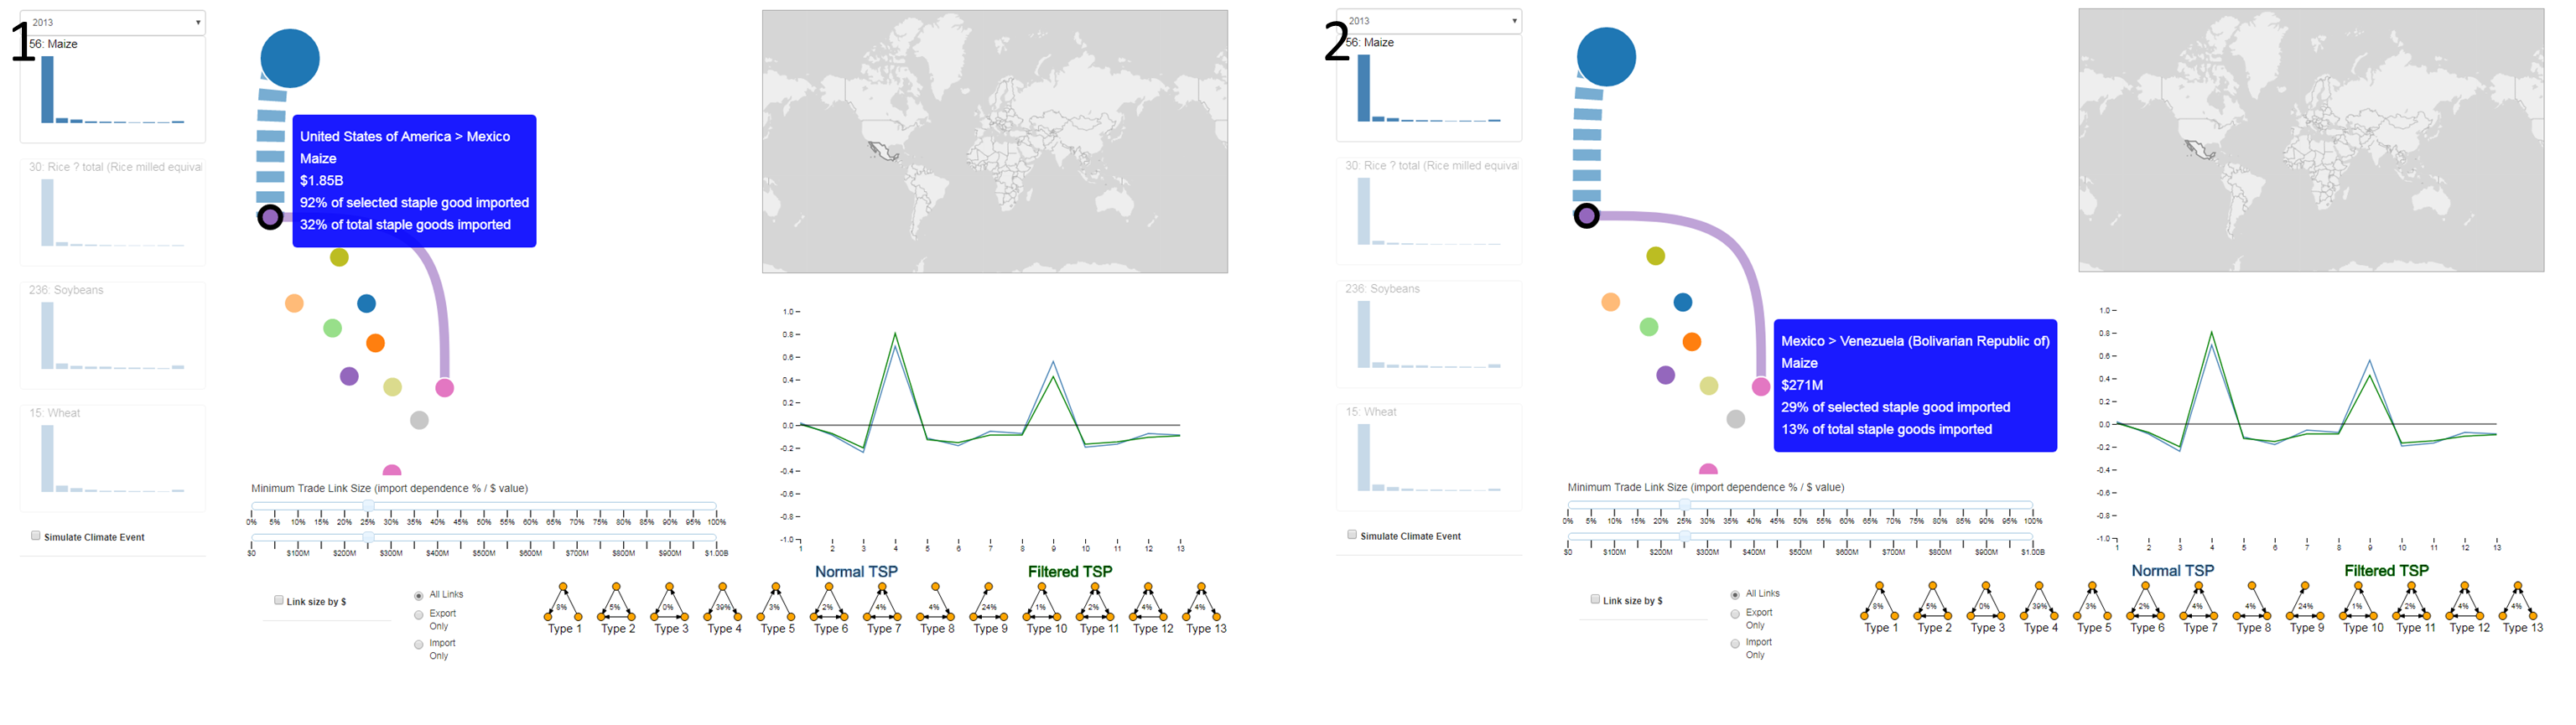
\includegraphics[width=\textwidth]{figures/mexico.png}}
				\caption[MEXICO AS A MIDDLE MAN FOR CORN]{A network graph showing corn that is imported or exported to Mexico(purple). The United States is shown in blue and Venezuela is shown in pink. The network graph has Mexico as the selected country and is filtered to only include export trade links that account for greater than 25\% of the link's importing country's total imports of the trade good. The large dashed line into Mexico shows that Mexico is highly dependent on the United States for a large portion of its corn (92\% from 1, tooltip). The solid line into Venezuela shows that Venezuela is moderately dependent on Mexico for corn (29\% from 2, tooltip).}
				\label{mexicoMiddleMan}
			\end{figure}
		\subsection{Choropleth Map (Section 3, Figure \ref{map})}
		\begin{figure}[htb]
			\center{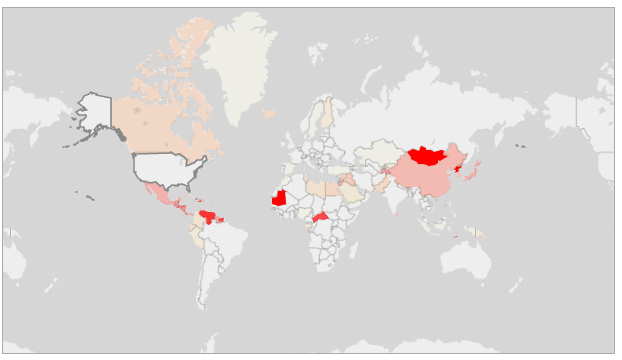
\includegraphics[width=\textwidth]{figures/map.png}}
			\caption[CHOROPLETH MAP OF A SIMULATED UNITED STATES EXPORT REDUCTION]{The choropleth map indicates the impact of a simulated climate event in the selected country on the downstream trade links. In this instance the United States experienced a climate event that reduced the value of corn exports by 10\%. The darker and more red the country is colored, the greater the impact. In this simulation Canada, China, and some central African countries were the most impacted by the event.}
			\label{map}
		\end{figure}
		The choropleth map in Figure \ref{map} shows all countries. The choropleth map is always present, but only colored when a country is selected either here or in the network graph. The positioning in the network graph mirrors the topological layout here to aid in identification of countries without cluttering associated with labels. The choropleth map in Figure \ref{map} gives a visual representation of the vulnerability index by affecting the intensity of coloring based on the loss of imports due to the simulated export reduction from the selected country as defined in Equation \ref{vulnerability}. Anything above 10\% is red and the opacity increases beyond that. If the number of times to cascade is greater than zero, it is possible for the selected country to also be affected. The tooltips in this section show the total imports and exports of the selected good by the country. In the event of a simulation the affected import value, the affected import value to total import ratio, and the affected import value to total trade ratio (Equation \ref{vulnerability}) are also displayed.\par
		The choropleth map is used for identification of vulnerable countries based on the climate event simulated. The more intense and more red the coloring, the higher the vulnerability. \par
		An interesting example of this is Australia. Simulating a 25\% reduction in 2013 wheat exports (Figure \ref{australia}) results in the loss of nearly 95\% of Australia's wheat imports. This is because New Zealand loses \$38 million in wheat trade from Australia and since New Zealand overall exports only \$3 million all trade links are essentially removed in the simulation, including the trade link back to Australia. However, Australia is not colored in heavily in the choropleth map because the loss of the \$600,000 trade link is not a significant percentage of the \$5.79 billion total wheat trade Australia is involved in.\par
		\begin{figure}[htb]
			\center{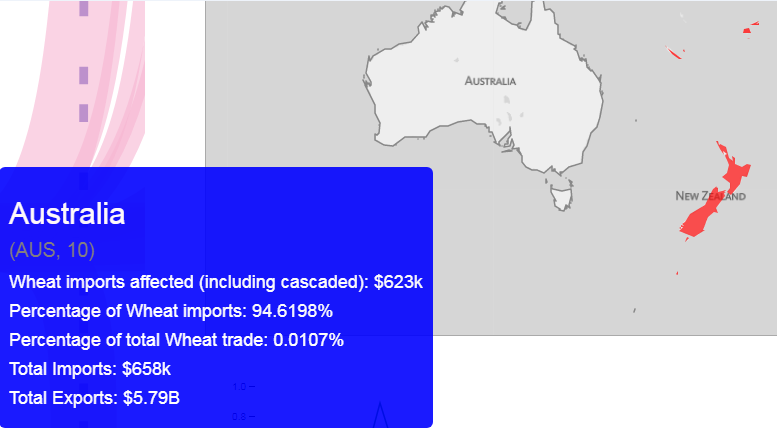
\includegraphics[width=\textwidth]{figures/australia.png}}
			\caption[CHOROPLETH MAP OF A SIMULATED AUSTRALIAN EXPORT REDUCTION]{In this simulation Australia experienced a climate event that reduced the value of wheat exports by 25\%. New Zealand is heavily affected and most of Australia's import links are broken. However, Australia is not colored in heavily in the choropleth map because the loss of the \$600,000 trade link is not a significant percentage of the \$5.79 billion total wheat trade Australia is involved in.}
			\label{australia}
		\end{figure}
	\subsection{Triad Significance Profiles (Section 4, Figures \ref{dashboardSections}-4, \ref{tsps})}
		Figure \ref{dashboardSections}-4 displays a normal triad significance profile (TSP) graph alongside the TSP graph for the current subset of data based on any filtering (e.g. selected country or minimum trade link size). In Figure \ref{dashboardSections}-4 the x-axis in the graph indicates the triad configuration type as shown in Figure \ref{triads}. Figure \ref{triads} shows the 13 different possible configurations in a directed network graph. In Figure \ref{triads} the triad distributions for the network graph of corn in 2013 are also shown. These percentages change based on the current subset of data. The y-axis in Figure \ref{dashboardSections}-4 shows the normalized z-scores defined as
		\begin{equation} \label{zScore}
			z_i=\frac{N^{actual} - N^{random}}{stdev(N^{random})}
		\end{equation}
		where $N^{actual}$ is the actual number of triads of this type and $N^{random}$ is the number of the same type in a randomly generated graph. A positive z-score indicates that the triads occurs more frequently than in a randomly generated network graph, and a negative value less frequently. The blue line shows the normal TSP for all 4 goods across all years of data and the green line is the TSP of the filtered data.\par		
		\begin{figure}[htb]
			\center{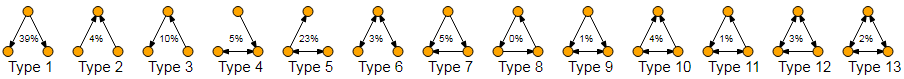
\includegraphics[width=\textwidth]{figures/triads.png}}
			\caption[13 DIFFERENT TRIADS]{The 13 different triads. The percentages here are the distribution of triads for corn in 2013. These values will change with the filtering of data.}
			\label{triads}
		\end{figure}
		Triad significance profiles can aid in the classification and comparison of the network across different types of systems \citep{shutters2012agricultural}. Certain motifs are more or less present in the superfamily identified. Being able to visualize the TSP of the currently filtered data may assist in an assessment of the health of the filtered trade links. Overall, the research in this thesis focused more on cascading impacts to the trade network, but future work will explore the impact of removing network connectors on distributions of triads.\par
		In the data for corn there are some interesting findings. In 1988 (Figure \ref{tsps}, left) we see one dominating triad, type one, which appears a lot more frequently than a random graph would suggest. Note that this triad does not include any bilateral trade links. Progressing from 1988 to 2013, we see the z-score of type nine, ten and thirteen, which all contain bilateral trade links, increase significantly (Figure \ref{triads}, right) and a decrease of type one and two, both unilateral triads. This may indicate an increasingly connected trade network. The increase of type three triads, in which the connecting node acts as a middle man, may suggest the possibility of cascading effects is increased.\par
		\begin{figure}[htb]
			\center{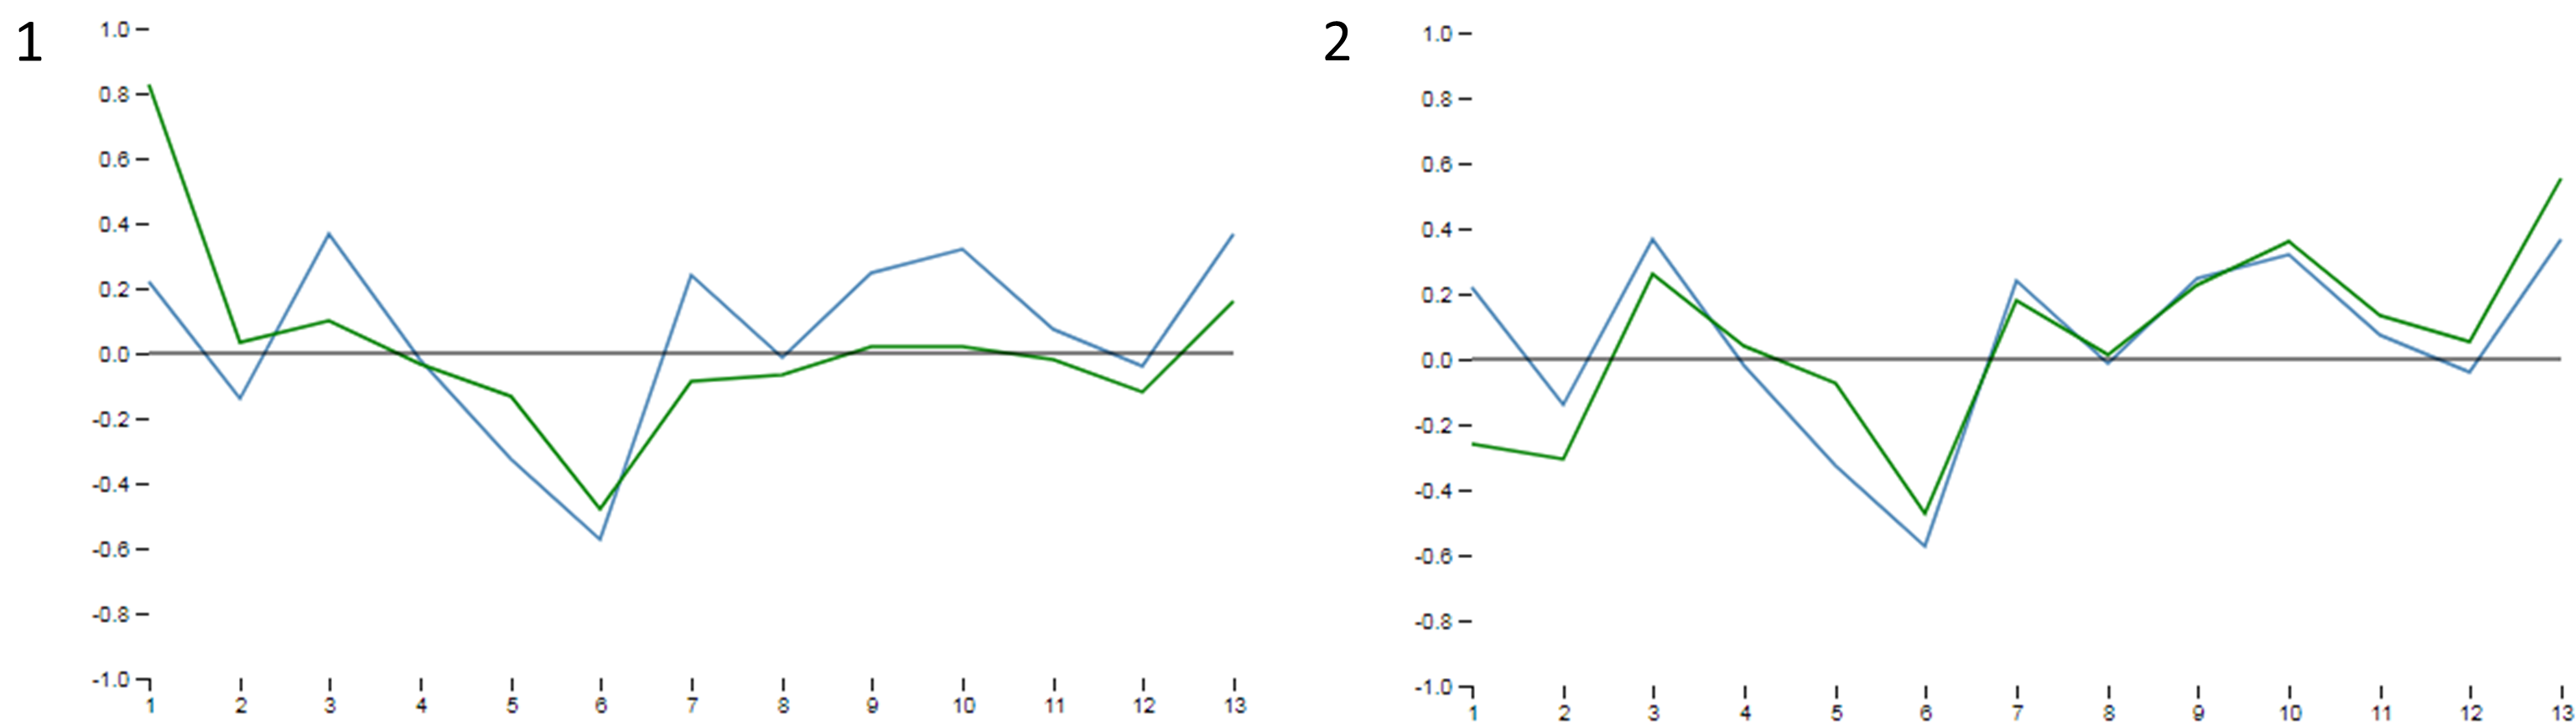
\includegraphics[width=\textwidth]{figures/tsps.png}}
			\caption[TRIAD SIGNIFICANCE PROFILES]{The is a graph that overlays the current triadic significance profile (TSP) with the normal TSP. The graph on the left is the 1988 wheat TSP and the graph on the right is 2013 wheat TSP. }
			\label{tsps}
		\end{figure}
\section{Enhancement Over Existing Visualizations}
	An emphasis of this visual analytics system is the consideration of the global trade network in its entirety. Neither of the reviewed visualizations take into consideration the topology of the food trade network. The FAOSTAT visualization represents only a single point in the food trade network. This does not allow for a direct interpretation of cascading effects. My tool visualizes the entire global trade network. The visualization offered by the Met Office \ref{metOffice} shows an index of food insecurity at a global scale. The focus is on overall vulnerability to food insecurity and does not visualize direct responses to climate events. The interaction and simulated climate events offered by my visual analytic system allow for the exploration of second-order effects of climate events by direct visualization of the affected trade links in the network graph and coloring in the choropleth map.\par
		
%\chapter{EXISTING TOOLS}
\label{existingVisualizationsChapter}
\section{Current Visualizations}
A number of visualization tools exist for exploration of food security, trade and climate change. Climate change models and future food insecurity indices are visualized on the \textit{Food Insecurity and Climate Change} website (figure \ref{metOffice}), hosted by the Met Office and World Food Programme (www.metoffice.gov.uk/food-insecurity-index). The website allows exploration of different scenarios of adaptation to climate change and greenhouse gas emissions. The visualization presents a long range (2050s and 2080s) forecast of the potential for food insecurity based on these factors.\par
\begin{figure}[htb]
	\center{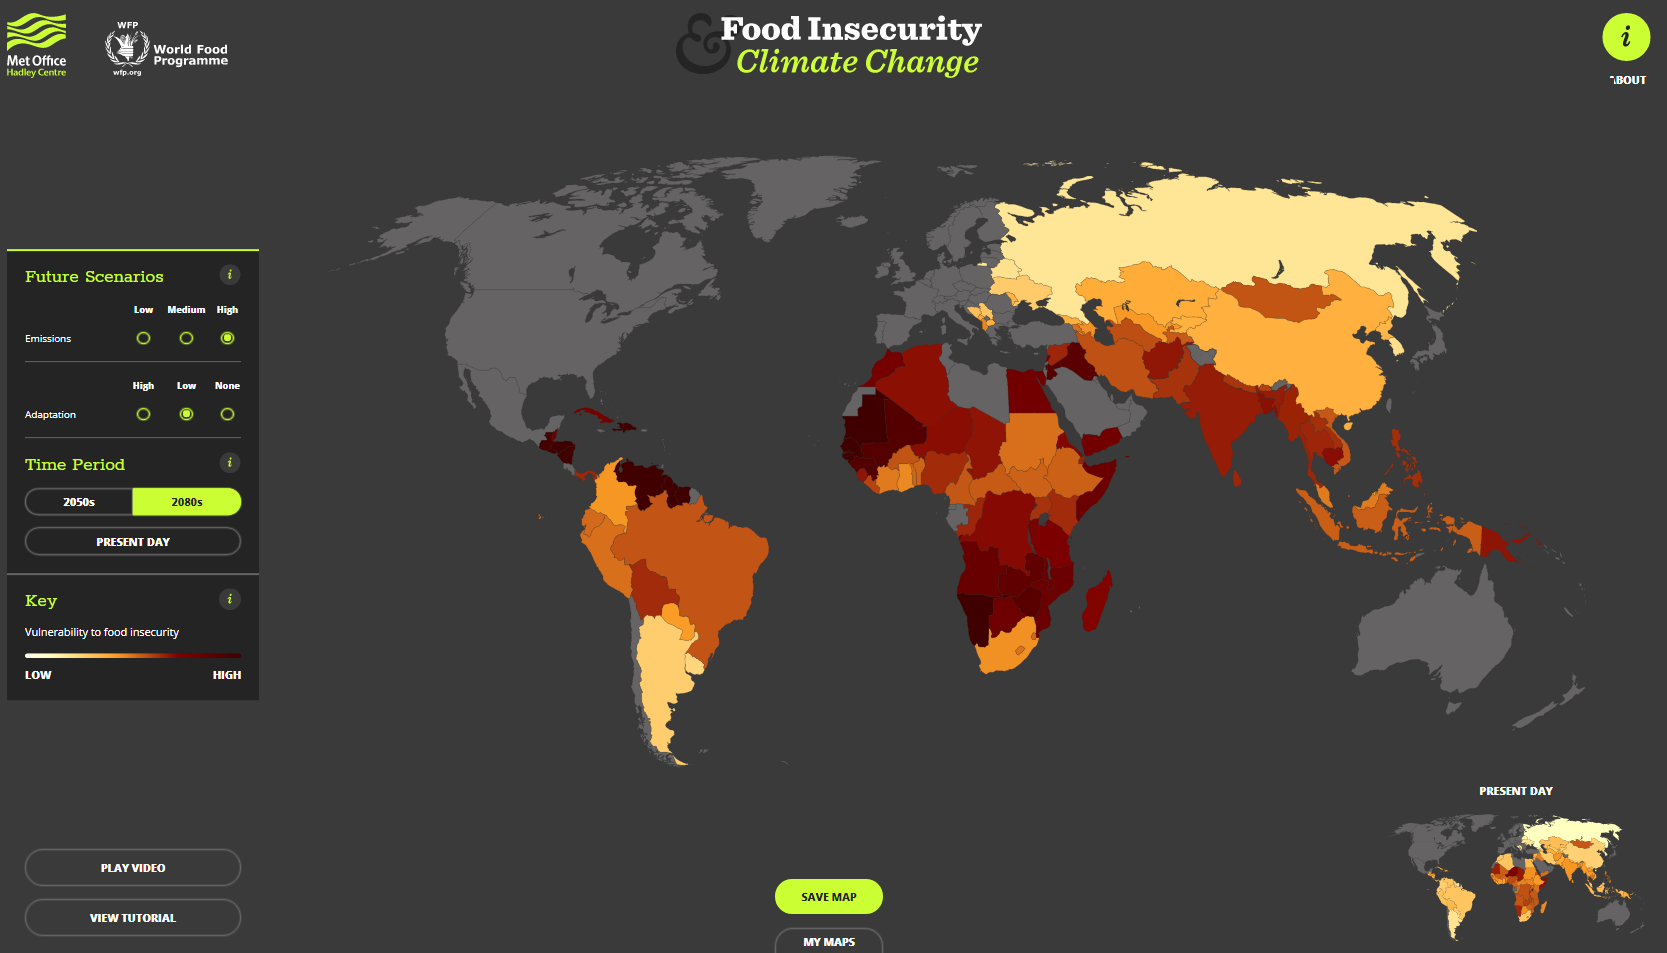
\includegraphics[width=\textwidth]{figures/metOffice.png}}
	\caption{Met Office Food Insecurity \& Climate Change website}
	\label{metOffice}
\end{figure}
Trade data can be visualized directly on the FAOSTAT website as seen in figure \ref{faostatViz} (www.fao.org/faostat/en/\#data/TM/visualize). This data visualization takes one country and displays the import or export trade links of a single trade good for that country. The visualization is done as a geographic choropleth representing the quantity or value of the imported or export good to another country. The visualization is limited as it only displays a single country's contribution and doesn't take into consideration the network as a whole.\par
\begin{figure}[htb]
	\center{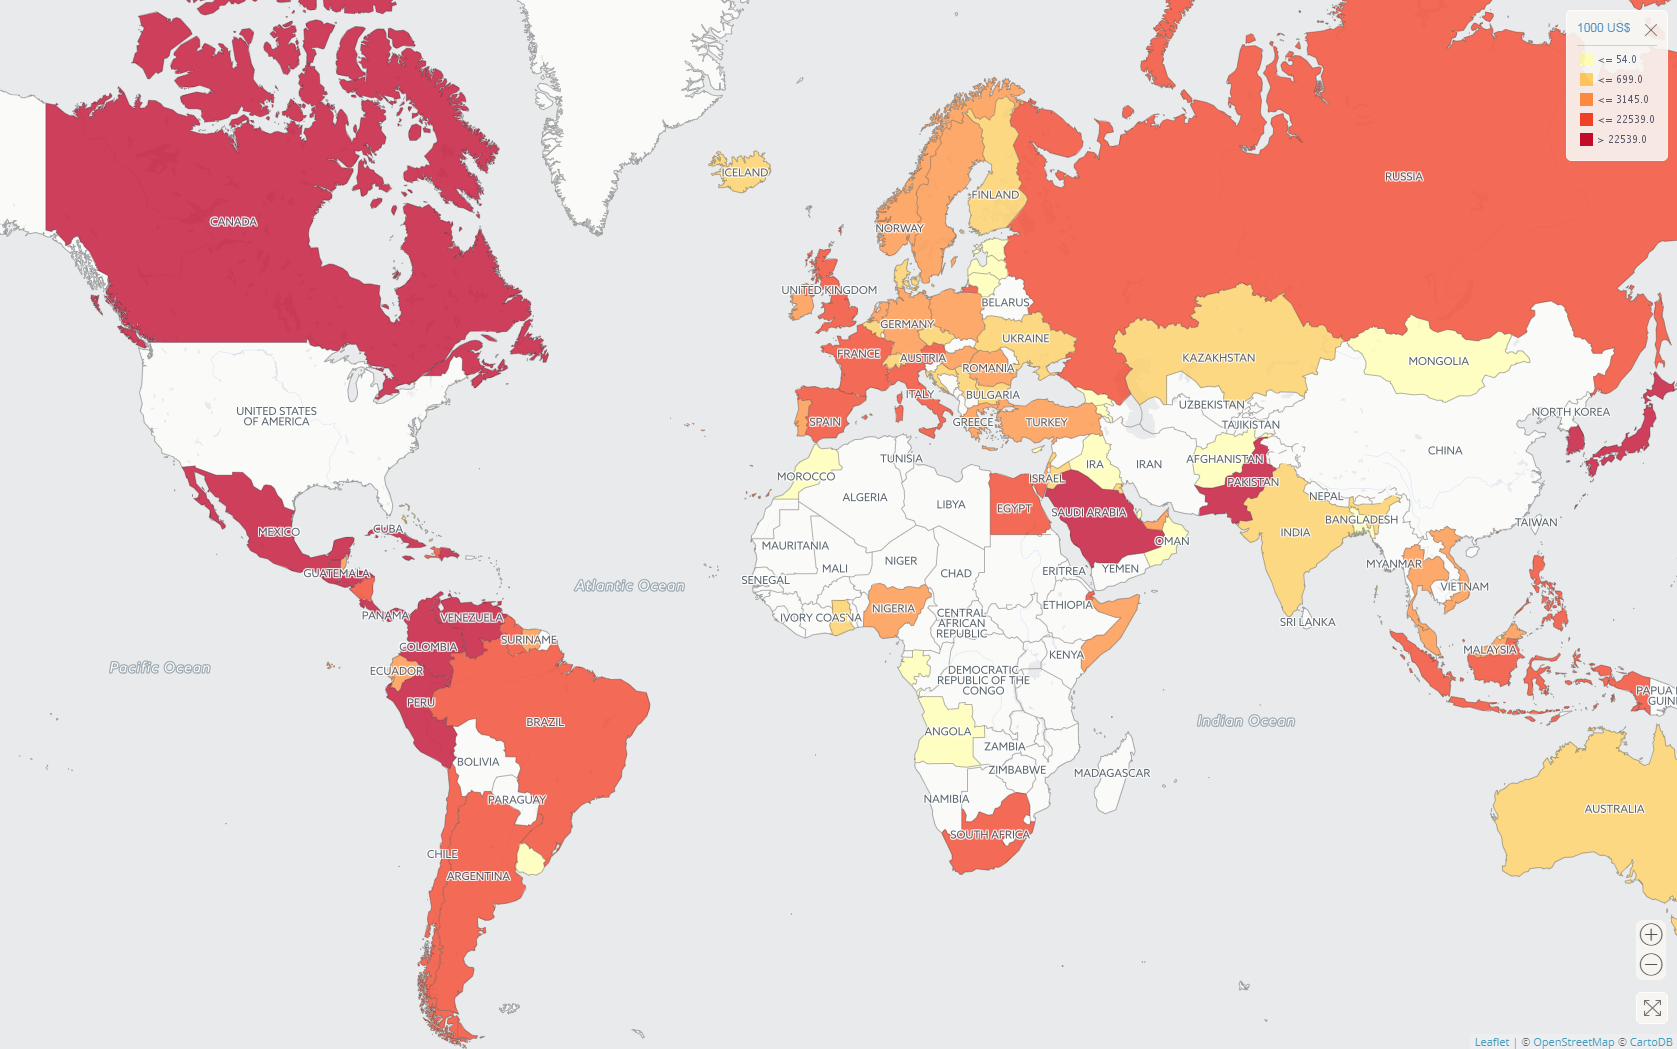
\includegraphics[width=\textwidth]{figures/faostatViz.png}}
	\caption{FAOSTAT Data Visualization tool}
	\label{faostatViz}
\end{figure}
\section{Enhancement Over the Existing Visualizations}
An emphasis of this visual analytics system is the consideration of the global trade network in its entirety. Neither of the reviewed visualizations take into consideration the topology of the food trade network. The FAOSTAT visualization represents only a single point in the food trade network. This does not allow for a direct interpretation of cascading effects. My tool visualizes the entire global trade network and allows for important network interpretations such as path length and network disconnections based on node and edge removal \citep{purchase1997aesthetic}. The visualization offered by the Met Office shows an index of food insecurity at a global scale. The focus is on overall vulnerability to food insecurity and does not visualize direct responses to climate events. The interaction and simulated climate events allow for the exploration of second order effects of climate events by direct visualization of the affected trade links in the network graph.\par

\chapter{CASE STUDIES}
\label{caseStudyChapter}
In this section two case studies are examined. The first is the 2011 Chinese drought and the second is a simulated future event where the United States corn exports are reduced. The first case study shows the basic use of the system and shows how we can identify vulnerable countries based on simulated climate events. Although the first case study does not highlight the cascading effects it does show that the vulnerability of a country may be affected by the simulation of a climate event. In our second case study we explore a full use case scenario of the system by targeting one of the largest corn exporters, the United States, and simulating a moderate climate event. In doing so we highlight the cascading effects to the food trade network and visualize the potentially vulnerable countries affected by a simulated climate event.\par
\section{2011 Chinese Drought}
In 2011 the United Nations’ food agency issued an alert warning that a severe drought was threatening the wheat crop in China, the world's largest wheat producer, and resulting in shortages of drinking water for people and livestock \citep{bradsher2011food}. In response to the drought China was forced to import more wheat instead of relying on its self sufficiency as in previous years \citep{sternberg2012chinese}. The increase in demand drives the price of wheat up as show in Table \ref{wheatTable}. This coupled with a number of countries implementing export bans the previous year \citep{fellmann2014harvest} has a great potential for a disrupted food trade network.\par
\begin{center}
	\begin{table}[htb]
		\centering
		\begin{tabular}{| c | c | c | c |}
			\hline
			Country & Market Year & Wheat Price USD / Ton & Exported to China (million USD)\\
			\hline \hline
			Australia & 2010 & \$200.00 & \$179\\ \hline
			Australia & 2011 & \$265.10 & \$180\\ \hline
			Australia & 2012 & \$235.00 & \$628\\ \hline
			Australia & 2013 & \$302.20 & \$242\\ \hline \hline
			Canada & 2010 & \$177.10 & \$72\\ \hline
			Canada & 2011 & \$237.00 & \$63\\ \hline
			Canada & 2012 & \$253.90 & \$163\\ \hline
			Canada & 2013 & \$252.90 & \$300\\ \hline \hline
			USA & 2010 & \$209.00 & \$36\\ \hline
			USA & 2011 & \$266.00 & \$159\\ \hline
			USA & 2012 & \$286.00 & \$224\\ \hline
			USA & 2013 & \$252.00 & \$1,292\\ \hline
		\end{tabular}
		\caption[WHEAT PRICE DATA FOR YEARS 2010 - 2013]{Wheat price data for years 2010 - 2013 (FAOSTAT Producer Prices - Annual) \citep{faostat}}
		\label{wheatTable}
	\end{table}
\end{center}
Halfway around the world in Egypt, the world's largest importer of wheat, was the resonance felt; wheat prices doubled the price of bread tripled \citep{sternberg2012chinese}. According to \cite{croppenstedt2006food} bread provides around one-third of the daily Egyptian caloric intake. These two factors prompted bread shortages and price increases in parts of the country that contributed to bread-inspired demonstrations and directly influenced political protest. \par
During this time many export restrictions were in place, including Russia's export ban \citep{fellmann2014harvest}. For simulation purposes, we model this export ban a 100\% export reduction out of Russia and run the simulation to see the vulnerable countries. Modeling it in this way allows us to see a number of countries significantly affected by the ban. Among them is Egypt, as anticipated, displaying an almost 40\% loss of imports (Figure \ref{egypt2011}, tooltip). From the red coloring in the choropleth map (Figure \ref{egypt2011}), the visual analytic system marks this as a potential area of vulnerability. Examining the network graph by filtering for very large links (great than \$500 million), Figure \ref{egypt2011-2013}-1 shows Egyptian imports of wheat from their main providers. In 2011 Egypt imports over \$2 billion from the United States and Russia. In 2013 that number is reduced to just \$1.1 billion. Though I make no claims of correlation, the 40\% reduction postulated from the simulation mirrors what is seen in Figure \ref{egypt2011-2013}.\par
\begin{figure}[htb]
	\center{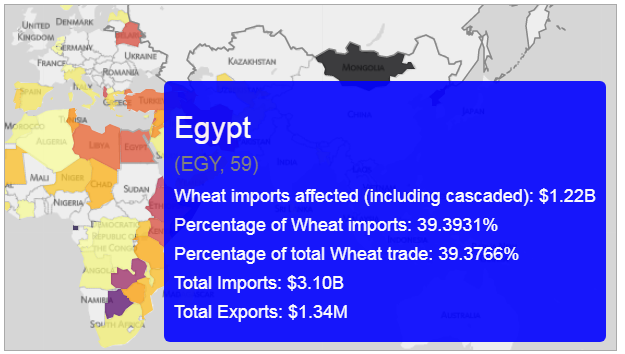
\includegraphics[width=\textwidth]{figures/egypt2011.png}}
	\caption[CHOROPLETH MAP OF SIMULATED RUSSIAN WHEAT EXPORT BAN]{Choropleth map of simulated Russian wheat export ban. The red color indicates that Egypt is moderately vulnerable to a climate event forcing an export reduction from Russia. The tooltip shows that Egypt would lose about \$1.22 billion in wheat imports accounting for almost 40\% of their entire import of wheat.}
	\label{egypt2011}
\end{figure}
Another aspect of analyzing the 2011 Chinese drought is supported by the system is exploration of the temporal changes to the food trade network by visualizing the graph year over year, as in Figure \ref{china2010-2013}, to look for patterns. We expect that there will be changes to the food trade network because of the aforementioned 2011 Chinese drought. The views in Figure \ref{china2010-2013} are set by selecting the first year to examine, 2010, and then filtered the network graph to only show links of greater than \$50 million. Each successive view only the year was modified.\par
As expected, looking at the graph we notice this sharp increase in imports of wheat to China. In 2010 China is largely self-sufficient; with imports of only \$296 million (Figure \ref{china2010-2013}-1, tooltip). In 2011 and 2012 we see still more increases in imports. Finally, moving to 2013, Chinese imports of wheat increased to \$1.90 billion (Figure \ref{china2010-2013}-4, tooltip), an increase of 640\%. The links go from virtually non-existent (figure \ref{china2010-2013}-1 US to China, \$56M in 2010, link not visible) to a trade link that is of a significant value (Figure \ref{china2010-2013}, bottom left; US to China, \$1.292 billion in 2013, large blue line). Moreover, from this progression we see the shift from Chinese self-sufficiency to import dependency.\par
From this case study we have demonstrated that our visual analytic system can help analysts explore the impacts of historical climate events on the international food trade network. 
\begin{figure}[htb]
	\center{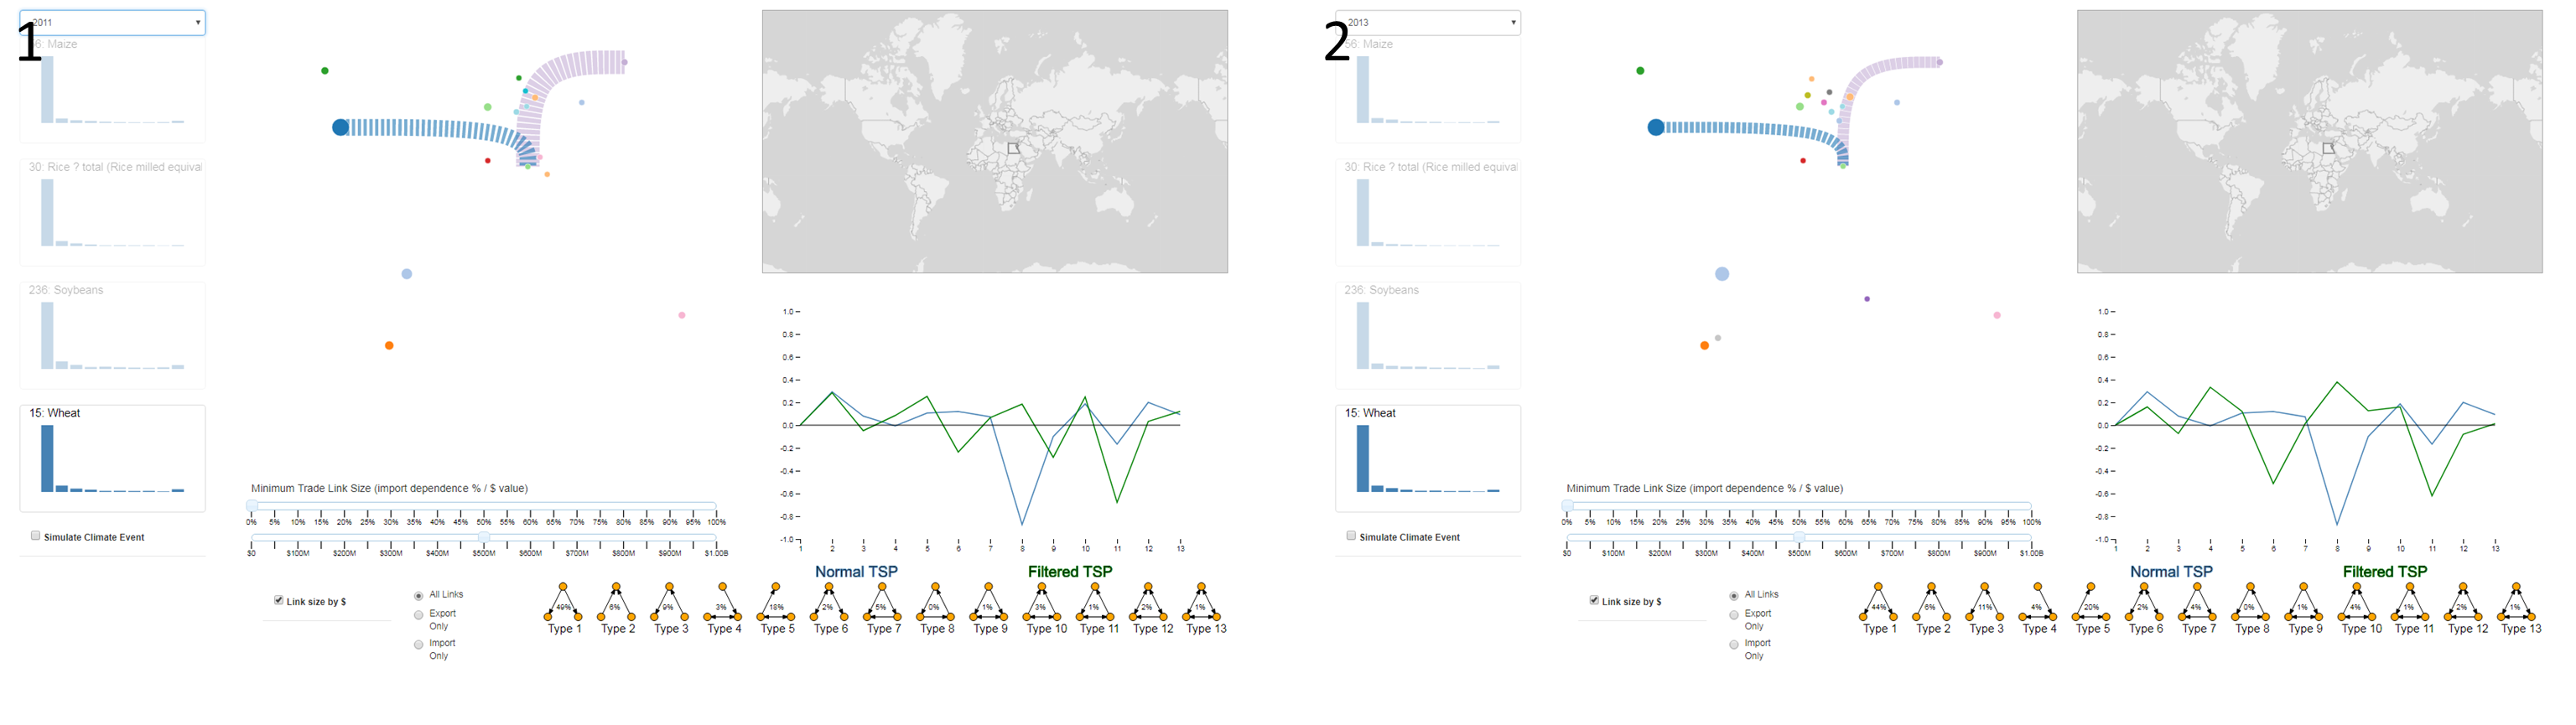
\includegraphics[width=\textwidth]{figures/egypt2011-2013.png}}
	\caption[PROGRESSION OF EGYPT WHEAT IMPORTS FROM 2011 TO 2013]{Left: {In 2011 Egypt (light blue) imports \$852 million in wheat from the United States (dark blue) and \$1.219 billion from Russia (pink). A total of approximately \$2.071 billion}; Right: {In 2013 Egypt (light blue) imports \$558 million in wheat from the United States (dark blue) and \$576 million from Russia (pink). A total of approximately \$1.134 billion is close to half of the value imported just two years ago.}}
	\label{egypt2011-2013}
\end{figure}
\begin{figure}[htb]
	\center{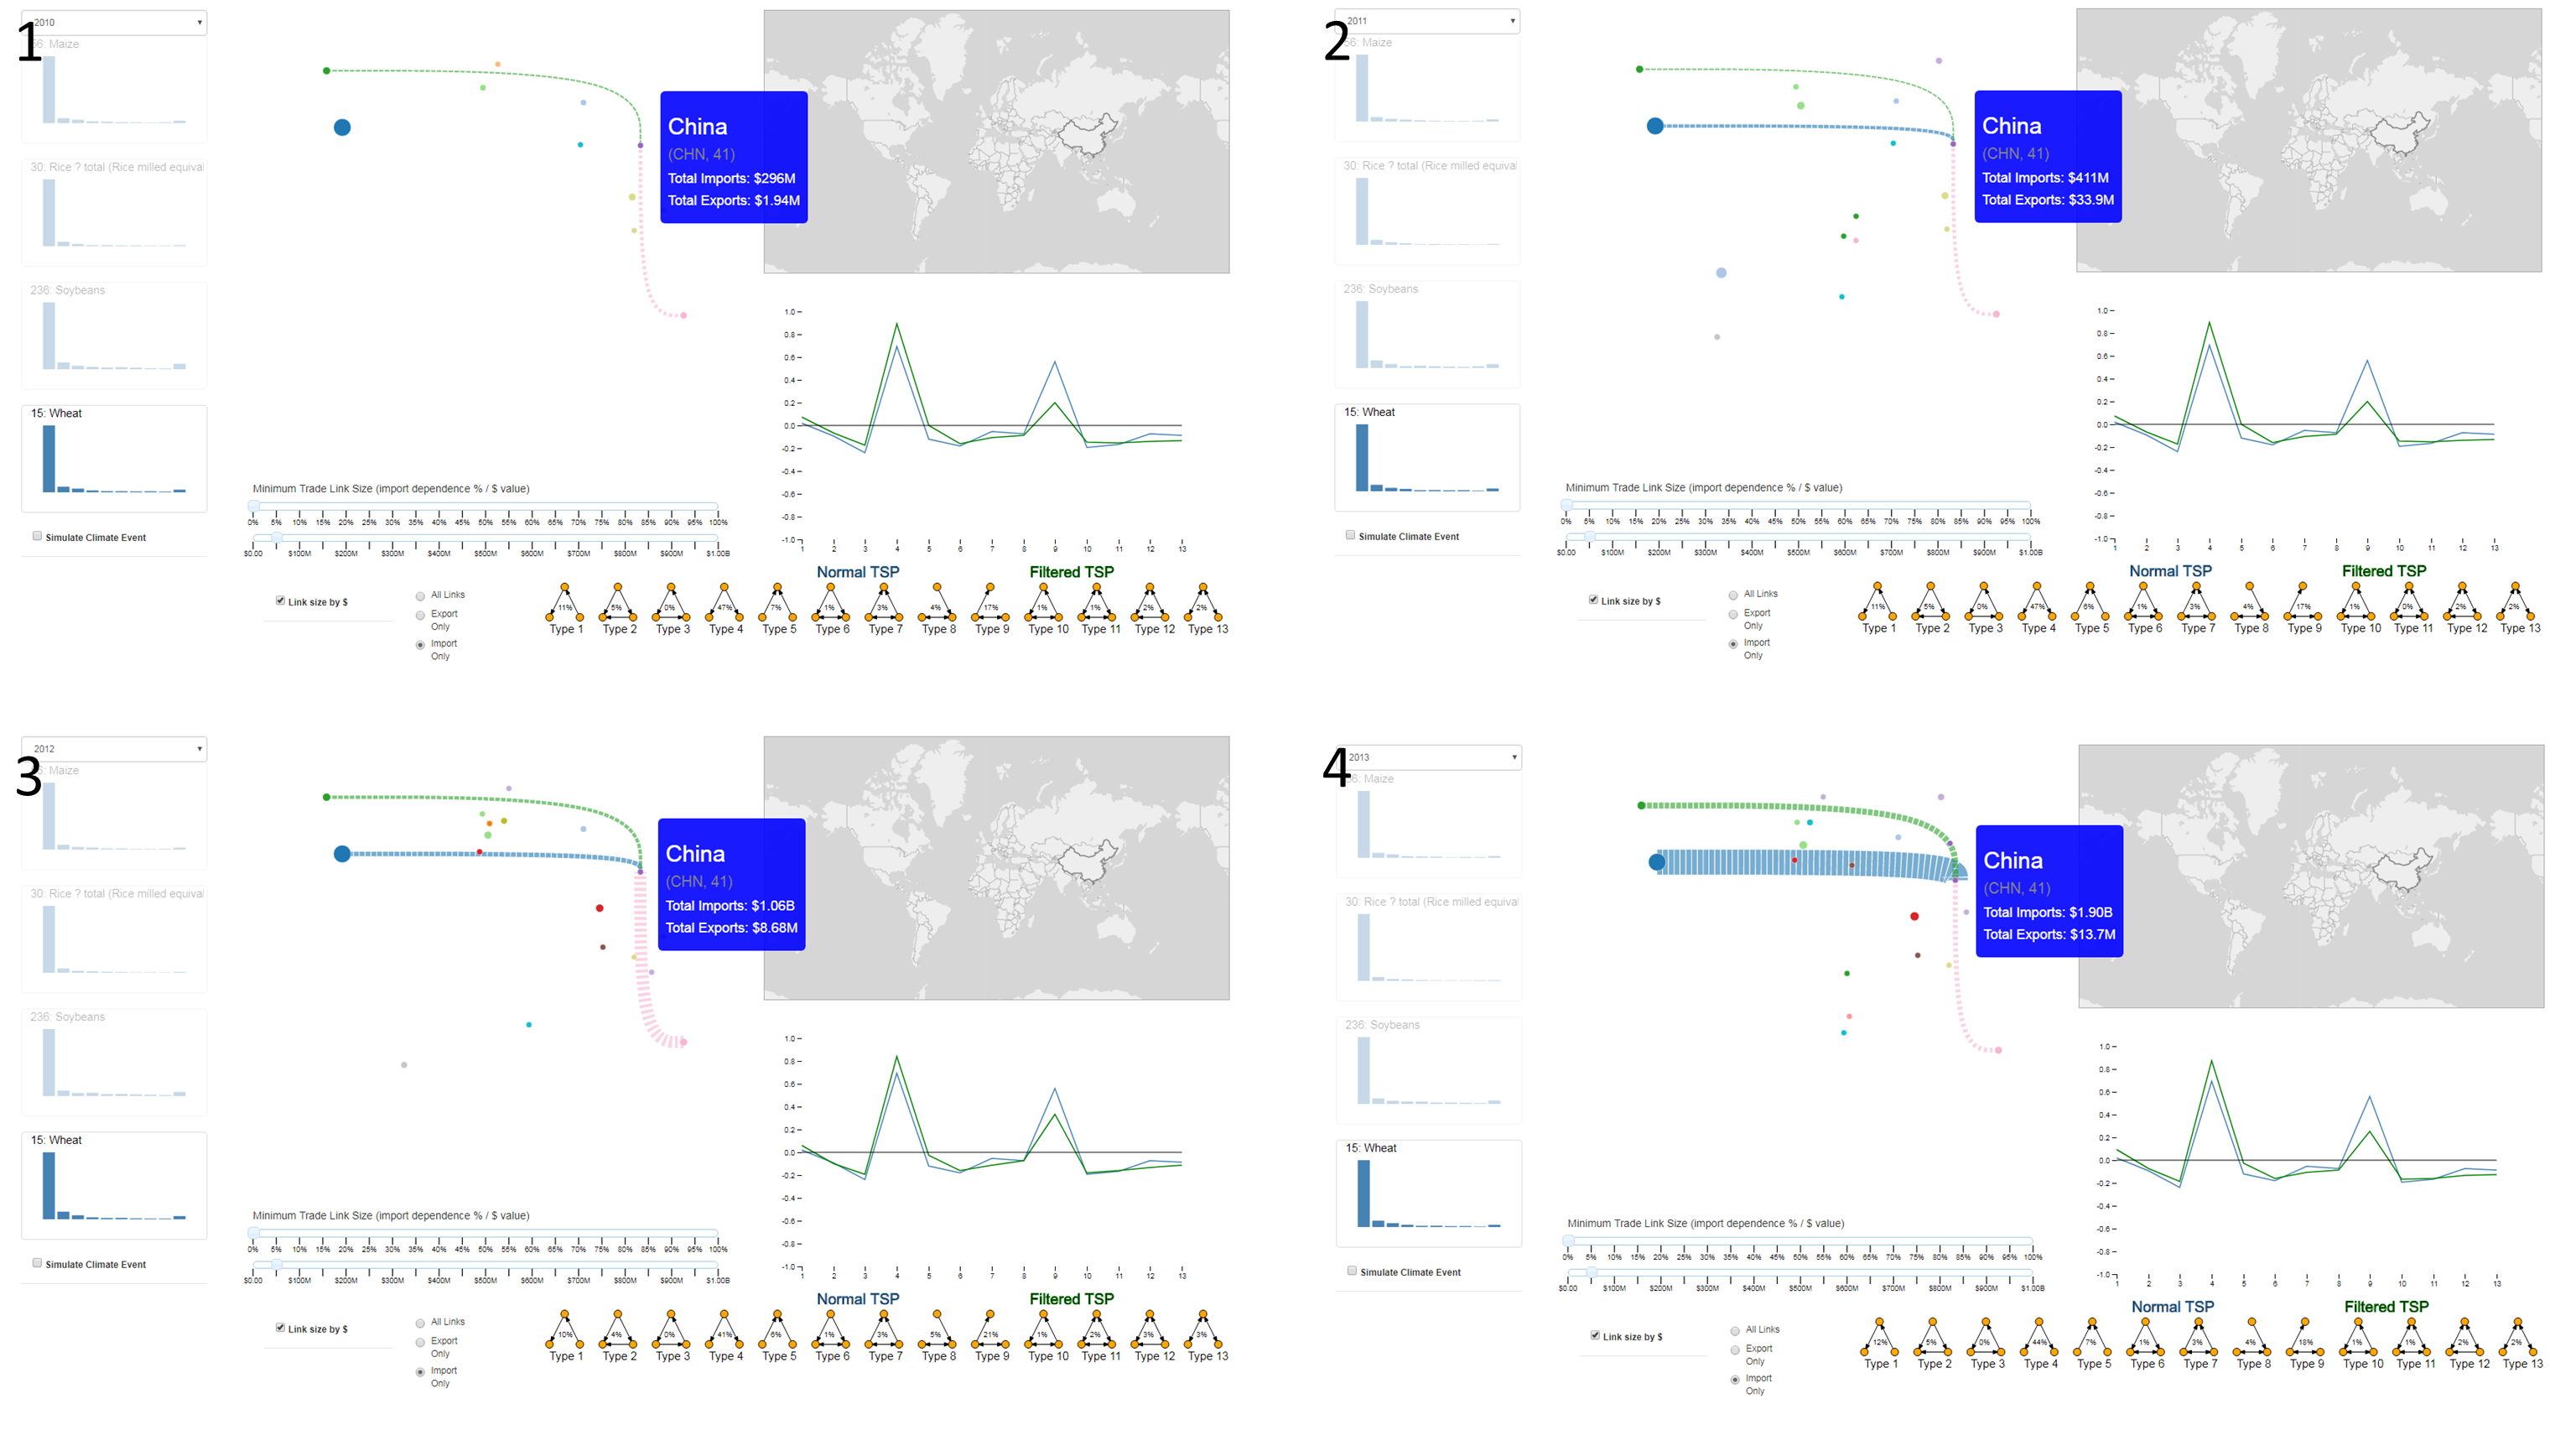
\includegraphics[width=\textwidth]{figures/china.png}}
	\caption[PROGRESSION OF SIGNIFICANT CHINESE WHEAT IMPORTS FROM 2010 TO 2013]{Progression of significant Chinese wheat imports from 2010 to 2013. Top Left: {In 2010 China (purple) imported \$36 million in wheat from the United States (blue, link not shown), \$72 million from Canada (green) and \$179 million from Australia (pink). From the tooltip China imported a total \$296 million}; Top Right: {In 2011, during the first year of the crisis, China (purple) imported \$159 million in wheat from the United States (blue), \$63 million from Canada (green) and \$180 million from Australia (pink). From the tooltip China imported a total \$411 million}; Bottom Left: {By 2012, with a sharp increase in imports directly related to the drought, China (purple) imported \$224 million in wheat from the United States (blue), \$163 million from Canada (green) and \$628 million from Australia (pink). From the tooltip China imported a total \$1.06 billion, almost four times the amount in 2010.}; Bottom Right: {By 2013 China (purple) being increasingly dependent on the \$1.292 billion imported from the United States (blue), \$300 million from Canada (green) and \$242 million from Australia (pink). From the tooltip China imported a total \$1.90 billion, a more than six-fold increase from 2010. }}
	\label{china2010-2013}
\end{figure}
\clearpage
\section{Simulated 2020 US Climate Event}
As a second case study, we will use the system to simulate the effect of an unspecified climate event to the United States. As a demonstration we will highlight the downstream effects of a major reduction in exports of corn from the United States.\par
Although the United States was chosen a priori, we could have used the 2013 trade data as a starting point to start the selection process for a country. This can be done by first inspecting the histograms. The tooltip in Figure \ref{cs2-0} shows three major importers, in both dollar value and import dependency, of United States' exports of corn: Mexico at \$1.85 billion and 92\%, China at \$1.05 billion and 91\% and Canada at \$281 million and 94\%. However, as import dependency is a function of the export value as well (Equation \ref{vulnerability}) we confirm import dependency on the network graph. To do so we filter the network graph to show only countries with an import dependence of at least 75\% and trade link values of at least \$100 million (Figure \ref{cs2-0}, sliders). Note that in this instance we could have filtered the network graph first, but using the histograms allows for the inspection of smaller countries. We do see two of the identified links still present (Figure \ref{cs2-0}, the two blue lines) with this filtering (the United States to Mexico and the United States to China) and so we decide to continue the analysis with the United States as the selected country. As the United States is one of the major exporters of corn (\$6.98 billion in 2013 according to the tooltip in Figure \ref{cs2-1}-1), we expect to see a number of vulnerable countries, even ones with no direct trade links with the United States. A 15\% export reduction is chosen arbitrarily as a starting point.\par
\begin{figure}[htb]
	\center{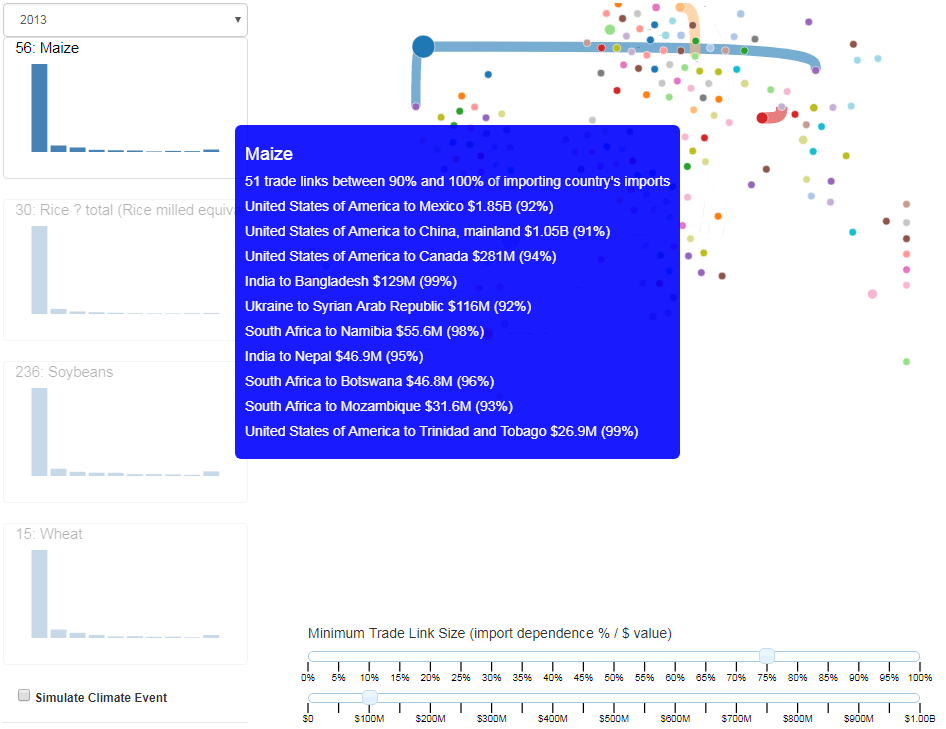
\includegraphics[width=\textwidth]{figures/selecting.png}}
	\caption[PROCESS OF SELECTING A COUNTRY FOR THE SIMULATION]{The process of selecting a country for the simulation starts with looking at the histograms and confirming on the network graph. Here the tooltip for the histogram displays the name of exporting and importing country along with the dollar value and import dependence of the trade link. This shows multiple potentially import dependent countries as indicated by a high import dependence percentage. The dependencies can be confirmed with filtering on the network graph (sliders on the bottom). The links remaining visible (the United States to Mexico, the United States to China, India to Bangladesh and Ukraine to the Syria Arab Republic) coincide with the histogram information.}
	\label{cs2-0}
\end{figure}
As the United States was chosen as a potential candidate for simulation, we select the node representing the United States (large blue node, approximately geographically positioned). The node and country in the map are drawn with dark borders to indicate it has been selected (Figure \ref{cs2-1}-1). As expected, and as shown in the network graph (Figure \ref{cs2-1}-1), there are a large number of countries involved in corn trade with the United States. Next the \textit{Simulate Climate Event} checkbox is selected and we select a 15\% reduction as shown in bottom left of Figure \ref{cs2-1}-2. The network graph in Figure \ref{cs2-1}-2 shows there are a large number of cascaded effects, represented by the now visible trade links. However, further filtering is required to gain context. In Figure \ref{cs2-1}-3 the \textit{Minimum Percentage of Imports Affected} is changed to 30\%. This filters the network graph to only display the links affecting those countries whose imports have been reduced by at least 30\%. Examining the choropleth map of the current state in Figure \ref{cs2-2}, we see that Venezuela, North Korea and Mongolia are affected heavily based on the darker coloring.\par
\begin{figure}[htb]
	\center{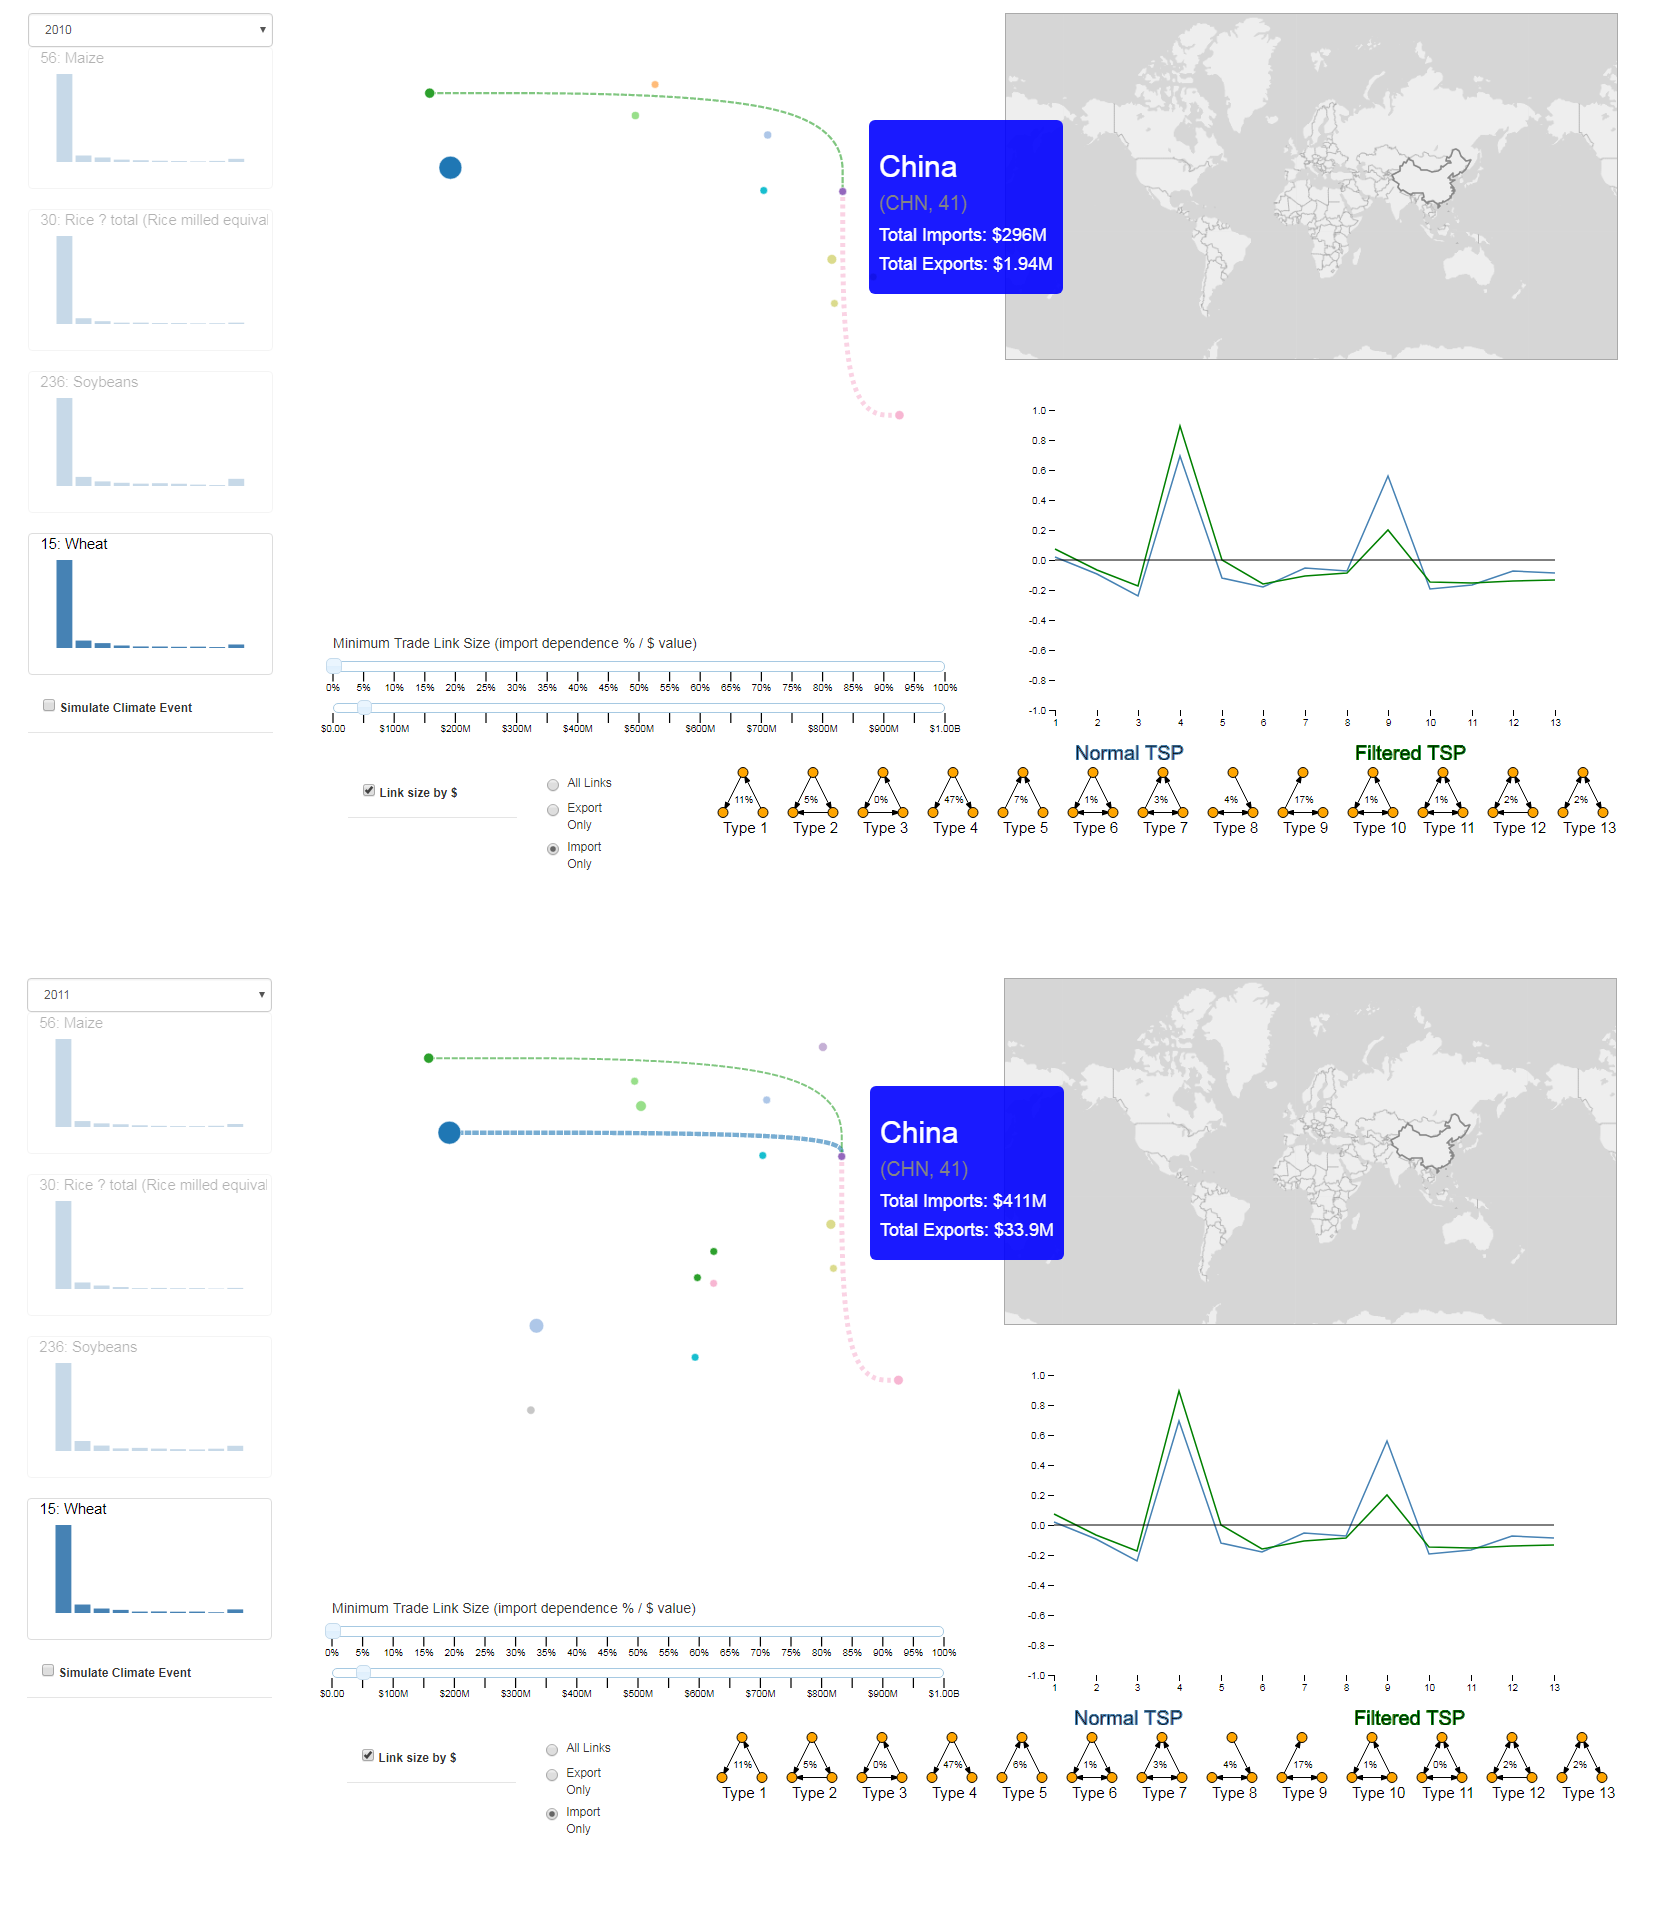
\includegraphics[width=\textwidth]{figures/cs2-1_tt.png}}
	\caption[RUNNING A SIMULATION AND EXPLORING RESULTS]{Running a simulation and exploring results. 1: {The United States is selected}; 2: {Simulation is ran with a 15\% export reduction from the United States}; 3: {Simulation results filtered on countries with import losses of at least 30\% and showing only links of at least a \$200 million dollar value}; 4: {Tooltip of the trade link from the United States to Venezuela} }
	\label{cs2-1}
\end{figure}
\begin{figure}[htb]
	\center{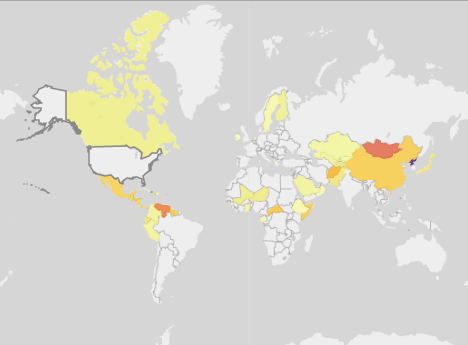
\includegraphics[width=\textwidth]{figures/cs2-2.png}}
	\caption[SIMULATION CHOROPLETH MAP]{A zoomed in view of the choropleth map from the simulation.}
	\label{cs2-2}
\end{figure}
To examine the impact on Venezuela we look at the trade links coming into Venezuela. The link from the United States shows a reduction of only \$55.5 million (Figure \ref{cs2-1}-4, tooltip), which is significantly less than the \$301 million shown in the country's information (Figure \ref{cs2-3}-1, tooltip). To look for other major import sources we slowly adjust the trade link size by dollar filter until only the top few links are shown (Figure \ref{cs2-3}-2, second slider has moved to \$200 million). Examining the link from Argentina to Venezuela (Figure \ref{cs2-3}-2, tooltip) shows a loss of only \$41k which has relatively little impact to the \$301 million loss. Examining the other link, Mexico to Venezuela, reveals the cascaded effect. Figure \ref{cs2-3}-4, tooltip, shows that Mexico's trade link to Venezuela has been reduced by \$240 million, a significant portion of the \$301 million total import loss to Venezuela. The export reduction of 15\% from the United States prompts a loss of \$280 million to Mexico (Figure \ref{cs2-3}-4) which is mostly passed on to Venezuela. Thus, Venezuela is indirectly impacted by a climate event to the United States, to the degree of approximately one third of their entire import of corn.\par
\begin{figure}[htb]
	\center{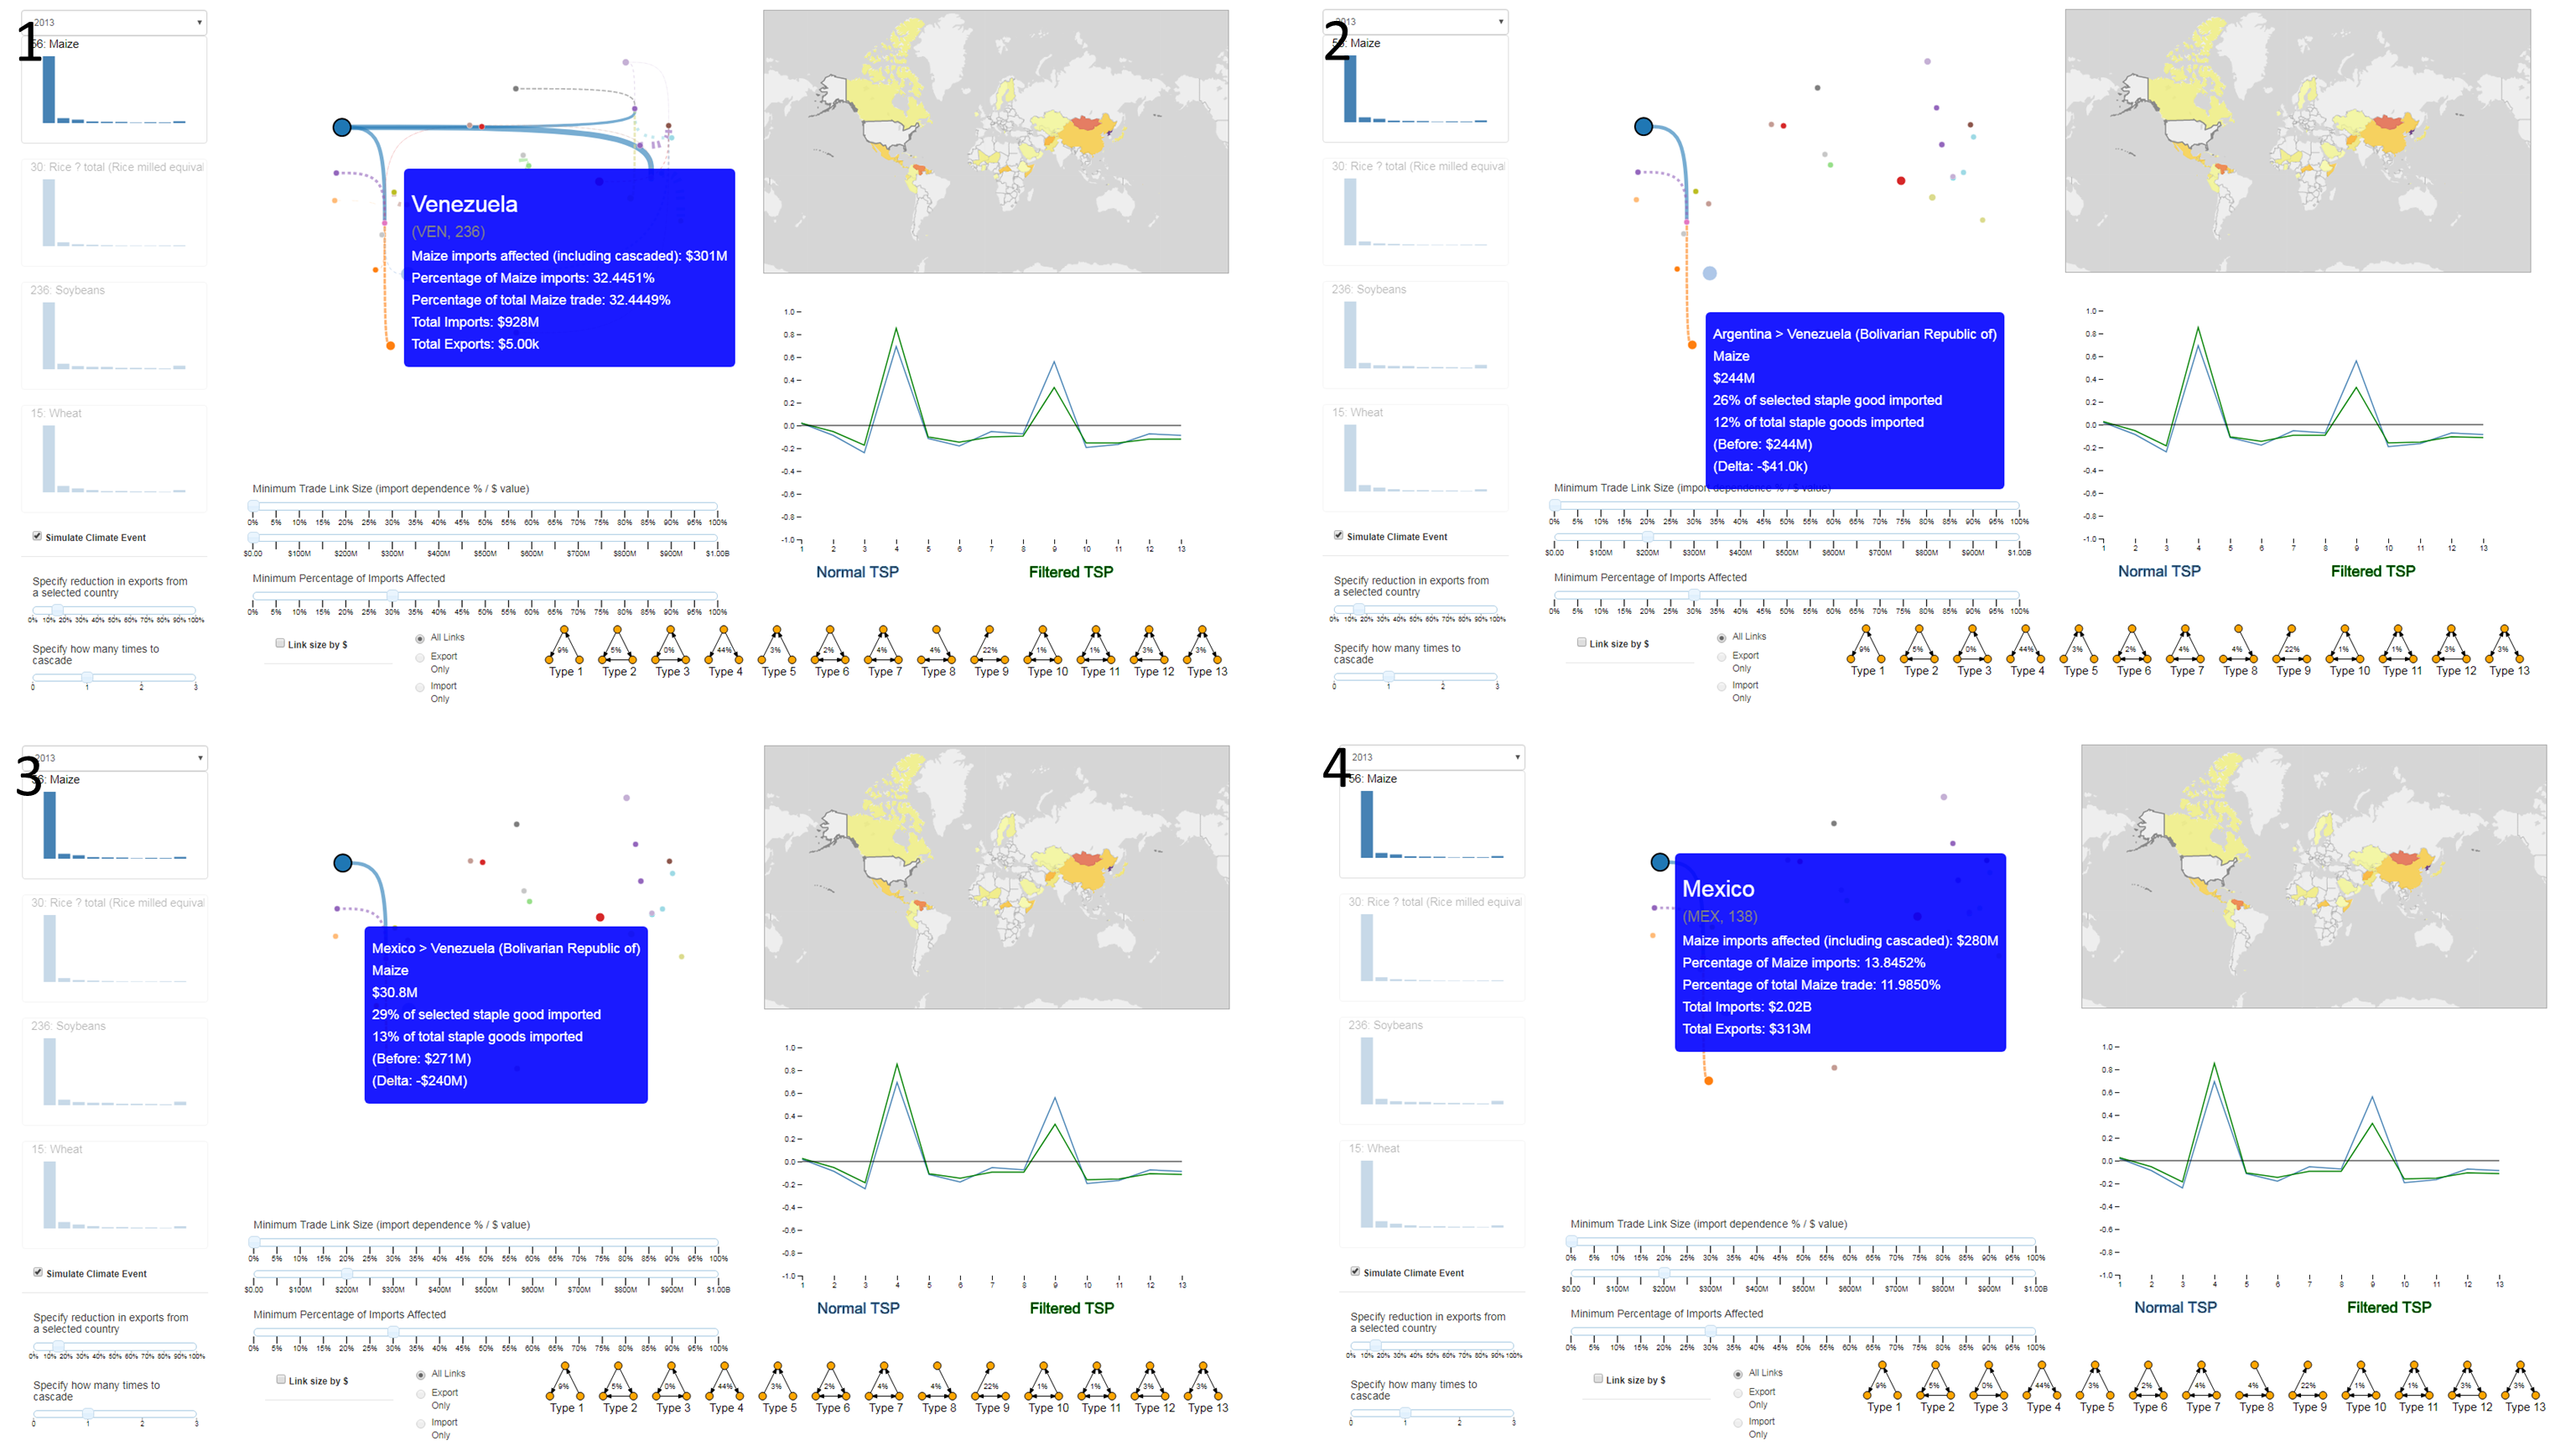
\includegraphics[width=\textwidth]{figures/cs2-3.png}}
	\caption[EXAMINING THE RESULTS OF A SIMULATION, FILTERED ON LARGE DOLLAR VALUE (\$200 MILLION) AND MODERATE IMPORT LOSSES (30\% LOSS)]{Examining the results of a simulation, filtered on large dollar value (\$200 million) and moderate import losses (30\% loss). 1: {Tooltip showing the impact to Venezuela}; 2: {Tooltip of the trade link from Argentina to Venezuela}; 3: {Tooltip of the trade link from Mexico to Venezuela}; 4: {Tooltip showing the impact to Mexico} }
	\label{cs2-3}
\end{figure}
Another example of use would be to see countries that are significantly (e.g. import losses of greater than 75\%) impacted by the climate event. We adjust the \textit{Minimum Percentage of Imports Affected} to 75\% (Figure \ref{cs2-4}-1) and \textit{Minimum Trade Link Size} to \$25 million to filter out the insignificant trade links. As indicated by the dark coloring in the choropleth map in Figure \ref{cs2-2}, the impact to North Korea is significant. However, no solid blue line (export from the United States) connects to North Korea (brown dot) in Figure \ref{cs2-4}-1 so no direct link exists from the United States to North Korea. Yet North Korea's imports are simulated to be affected by almost 80\% (Figure \ref{cs2-4}-2, tooltip). By examination of the link (Figure \ref{cs2-4}-3) we conclude that China acts as a middle man. The tooltip in Figure \ref{cs2-4}-4 shows that China lost imports of \$158 million. The same tooltip shows that it only exports \$34.2 million. Since the loss of imports is assumed to be first mitigated by reduction of exports, China essential breaks all export links to recoup the \$158 million loss of imports. This is a potential limitation of the system as China may still export the relatively small amount of \$31.9 million (Figure \ref{cs2-4}-3) to North Korea depending on a number of factors. (e.g. political repercussions, temporal considerations such as season). This example shows the cascading effect of the loss of imports to China from the United States being propagated to North Korea.\par
\begin{figure}[htb]
	\center{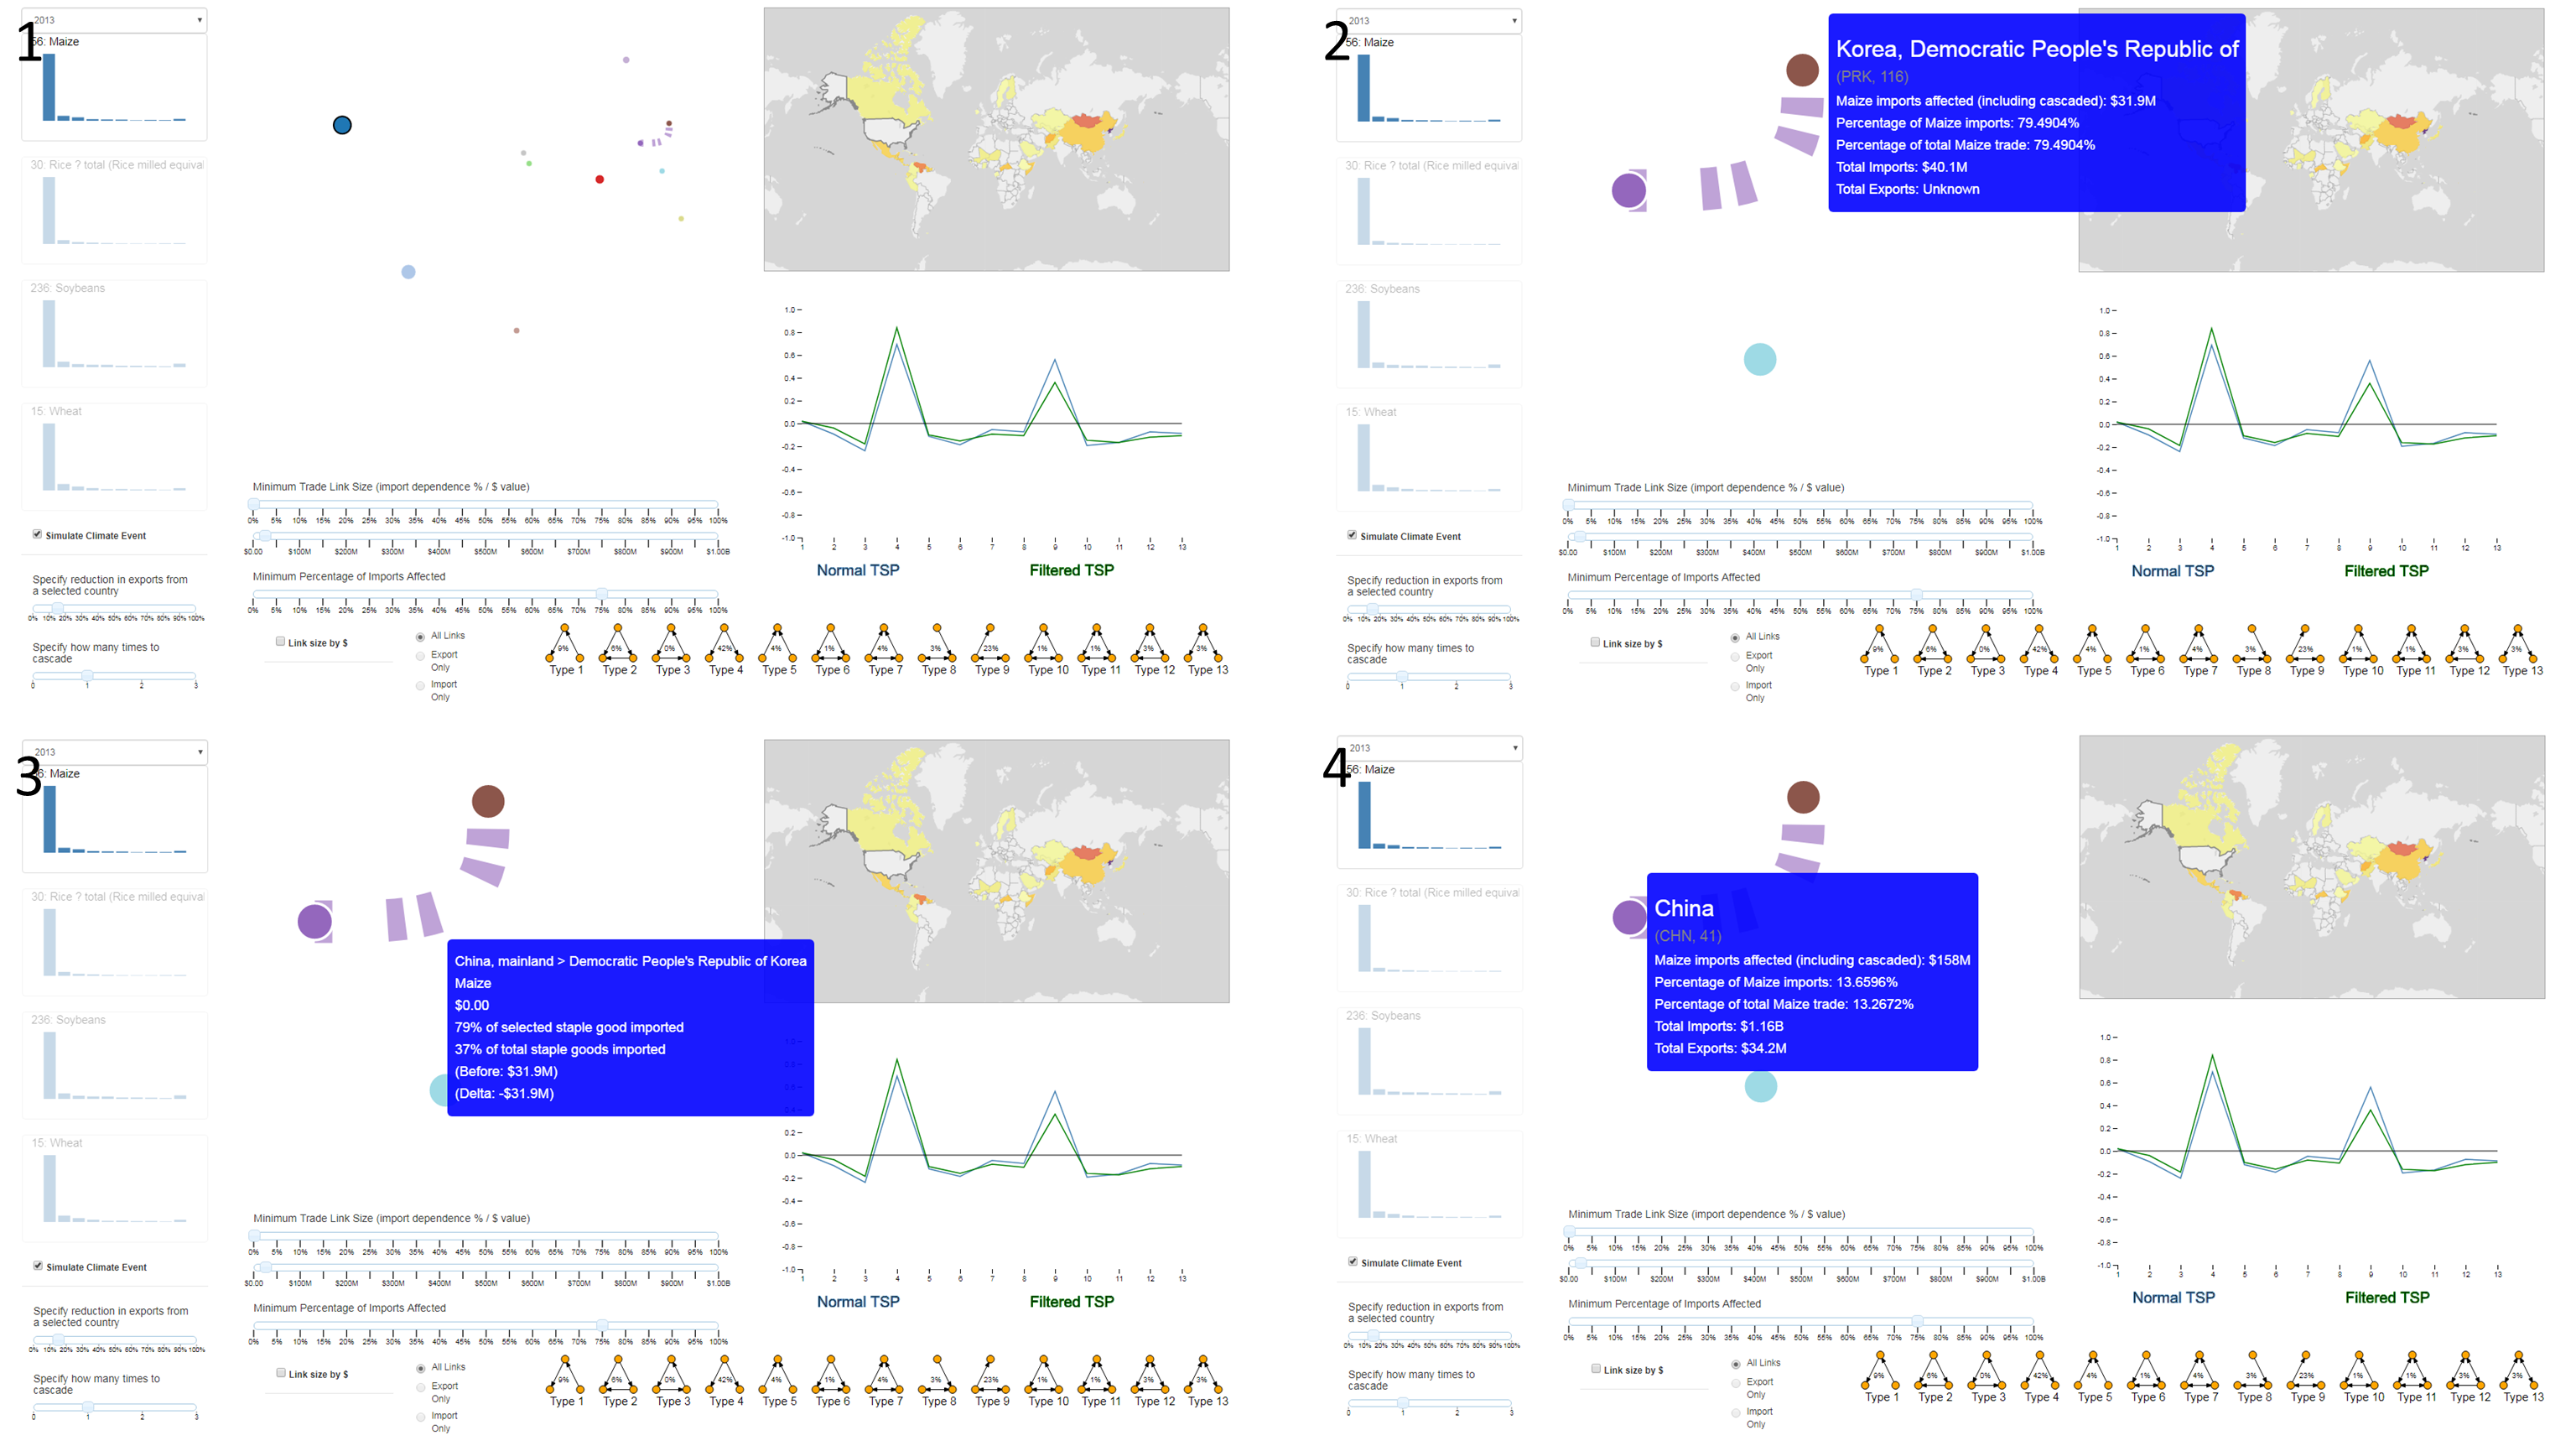
\includegraphics[width=\textwidth]{figures/cs2-4.png}}
	\caption[EXAMINING THE RESULTS OF A SIMULATION, FILTERED ON MODERATE DOLLAR VALUE (\$25 MILLION) AND LARGE IMPORT LOSSES (75\% LOSS)]{Examining the results of a simulation, filtered on moderate dollar value (\$25 million) and large import losses (75\% loss). 1: {Simulation results filtered on countries with import losses of at least 75\% and showing only links of at least a \$25 million dollar value}; 2: {Tooltip showing the impact to North Korea. The link is also drawn with alternating dashes and spaces, indicating it has been broken.}; 3: {Tooltip of the trade link from China to North Korea}; 4: {Tooltip showing the impact to China} }
	\label{cs2-4}
\end{figure}
This case study highlights the usefulness of these cascading, second-order effects. In the example of Venezuela we are able to see that Venezuela is more heavily affected than the direct trade link would suggest. In the example of North Korea there is no direct trade link and without cascading effects being accounted for, the vulnerability to North Korea may not be considered at all. The ability to visualize these links facilitates the identification of these potentially vulnerable, import reliant countries. This is even more apparent when those countries are dependent on a small number of suppliers as seen in both cases presented here.\par

\chapter{CONCLUSIONS}
\label{conclusionsChapter}
\section{Summary}
The goal of this thesis was to allow for effective visualization of the international food trade network, identification of potentially vulnerable countries and aid in prediction of level of food insecurity risk based on impacts of future climate variability. To achieve this goal a visual analytics framework was created for visual analysis and exploration of the network. This framework allows the domain expert to filter and manipulate the dataset. It also allows for a level of prediction by simulating the effect of a climate event. The framework helps determine downstream effects of a reduction in one country's exports beyond the first level of trade.\par
\section{Limitations}
The simulations on the dashboard are limited in scope to a single country and single staple good. In the case study of the 2011 Chinese drought this was an apparent limitation. It is known that there were a number of countries implementing export bans \citep{fellmann2014harvest} based on the climate event and being able to model all in one simulation would draw a better representation of the state of the global food trade network at the time. This would facilitate more accurate vulnerability modeling. Disallowing multiple crop types also is a limitation. Being able to work with all four of the staple goods at one would allow for exploration of gap coverages in staple crop imports. It would also allow a truer picture of the effect to food security to a country based on the simulated climate event.\par
There are also a number of limitations encompassed on the graphical user interface of dashboard. The majority of the computation of downstream effects is done on the front-end. This makes processing of the cascading links CPU intensive and anything beyond two iterations the dashboard becomes unresponsive. Holding such a large number of links in memory client side forces the inspection of a singular trade good at one time. Creation of such a large number of network graphs links as DOM elements allows for the interactivity of the dashboard but rendering on a HTML5 canvas would perform much better. This is also a limiting factor in the scalability of the network graph representation. Only the display of the four staple crops were chosen for this reason.\par
\section{Future Work}
There is a lot of potential for future enhancements. Addressing the above limitations would be the primary focus. The ability to add intelligence to weight trade links based on some criteria to allow for unequal distribution of remaining trade goods as a result of a climate event is another. This could potentially be achieved by geographical proximity or known relationship statuses between countries. In the choropleth, the visualization could also take into account other traditional vulnerability indices to affect the intensity of coloring.\par
Another avenue of future work would be to further explore network triad distributions and triad significance profiles (TSP) related to the international food trade network. For instance, how do changes to the international food trade network based on simulated climate events alter the distributions? Are the TSP affected as well and is there a change in motifs? Are there any patterns related to vulnerability and entrance to or exit from motif positions based on altered trade links?\par
Another potential improvement would be to affect the production of food goods instead of just export link value. Food production could be limited to a point where there is actually a greater reduction in exports that the static loss of production. An example of this would be Russia's recent ban on exports of wheat during the 2011 drought to stabilize internal stores. FAOSTAT also has the production data in their database and being able to incorporate this data, along with population statistics, could prove very useful.\par
Another option would be improvement of the algorithm for the distribution of the remaining exports. It may not be realistic to assume that the country experiencing the export reduction would perfectly distribute the remaining exports among their trade partners. In reality the distribution of exports may be skewed towards the most proximal country or, more likely, the country willing to pay the most.\par
Another significant enhancement would be able to enhance the algorithm to associate water dependency of crops more accurately. Virtual water, the amount of water embedded in a particular good, is a current area of research and the system could be adapted to consider the virtual water as in the current well-defined models \citep{hoekstra2005globalisation}. Alternatively if one crop is more dependent on water there could be a coefficient of impact to take that into account. Other research, such as \cite{konar2011water}, has sought to explore the food trade in relation to the virtual water value of the commodity. Future research may make this conversion to account for not only reduction but possible increases in crop production.\par
The system could also be improved to take into account the temporal aspects of crop production. For instance, is the same good being traded between counties because of different growing seasons? Is a country more import dependent on different countries based on the time of year? There is potential to model the simulation based on the production of a crop, the season, and the geographical location.\par
As mentioned in the introduction, the scope of this system is not limited to climate events or food trade. The system could be expanded to allow for trade of other goods, such as raw materials. This is particularly true if we are able to map a raw material to a production good. As an example, in the event of a reduction in silicon imports to a country, how could we model the reduction in computer chips, made with silicon, exports from that country? This is another cascading effect that may benefit from analysis.\par
%	Mechanisms for coping with food crises include direct provision of food aid \citep{timmer2010reflections}. However this international aid needs to be directed. Many times the most affected regions are not proximal to the climate event but geographically separated.\par


In chapter \ref{relatedWorkChapter} a literature study is conducted with a high-level summarization of related works. In chapter \ref{foodTradeNetworkChapter} an introduction to the international food trade network is given. Chapter \ref{networkAnalysisChapter} analyses the international food trade network with respect to network graph theory. Chapter \ref{effectiveVisualizationsChapter} emphasizes properties of effective visualizations that led to the design of the dashboard. Chapter \ref{systemChapter} illustrates the system architecture. The Chinese drought is explored as a case study with the tool in chapter \ref{caseStudyChapter}. Finally chapter \ref{conclusionsChapter} summarizes this work.

\section{Indicators of Vulnerability}

\subsection{Food Security}
\subsubsection{Food Availability}
National average DES (dietary energy supply). FAO defined minimum dietary energy requirement (MDER) (1844 kcal/cap/day) and average dietary energy requirement (ADER) (2353 kcal/cap/d) for the period of 2014-2016.
Two ways to obtain: a) domestic production and b) benefit from food trade, either from income of food exports or import of external resources. \cite{porkka2013food}
\subsubsection{Food Self-Sufficiency}
Dietary energy production (DEP) compared to global ADER
Low production: DEP of less than 2000 kcal/cap/d
Insufficient production: DEP of 2000–2500 kcal/cap/d
Sufficient production: DEP of 2500–3000 kcal/cap/d
High production: DEP of over 3000 kcal/cap/d \cite{porkka2013food}
How to change: Average value of food production -> DEP
Low self-sufficiency + (high export single good?)
\subsubsection{Food Trade}
High net imports: DES – DEP of over 1500 kcal/cap/d
Moderate net imports: DES – DEP of 500–1500 kcal/cap/d
Low net imports: DES – DEP of 0–500 kcal/cap/d
Low net exports: DEP – DES of 0–500 kcal/cap/d
Moderate net exports: DEP – DES of 500–1500 kcal/cap/d
High net exports: DEP – DES of over 1500 kcal/cap/d \cite{porkka2013food}
\subsubsection{Composition of Diet}
Average supply of protein of animal origin: Food\_Security\_Indicators.xlsx

\subsection{Climate Change Vulnerability Indicators}
Enumerate these more better.
\subsubsection{Indicator 1}
\subsubsection{Indicator 2}
\subsubsection{Indicator 3}

\subsection{Agricultural Vulnerability to Climate Change}
Introduce composite index methods and assessment of each with \cite{wirehn2015assessment}.
\section{VISUALIZATION}
\subsection{Geospatial}
Why use geospatial?
\subsection{Network}
How to incorporate nodes/edges in geospatial effectively.
Motif simplification. \cite{dunne2013motif}
\subsection{Chloropleth v. Size of Nodes}
Or some other way to indicate a relative value.
\subsection{Effectiveness}
Using information from \cite{preston2011putting} defend why this is an effective method for displaying the data.



This general question can be split into several sub-questions, which are listed below.\par
Research questions:
\begin{itemize}
	\item Which “climate singularities” have an impact on the agricultural trade network? Is the impact limited to droughts or are there other relevant atmospheric events?
	\item How far-reaching is the impact of each of these climate singularities, if it appears in a specific region of the world? The import and export of which countries (= nodes of a weighted graph) will be impacted, and to which extent?
	\item How can such singularities and their impact be projected to the future, using statistical modelling?
	\item How can integrated climate and agricultural trade data be visualized, and how does this visualization facilitate the ongoing analysis?	
\end{itemize}\par
\section{Research Plan}
\begin{enumerate}
	\item Literature review
	\begin{itemize}
		\item World trade networks
		\item Climate change*
		\item Algorithms for weighted graphs*
		\item Geospatial network visualization
		\item Time series analysis and modeling*
	\end{itemize}
	\item Determine research methodology concerning graph algorithms and statistical modelling
	\begin{itemize}
		\item How to find “climate singularities”?
		\item How to correlate these singularities with the agricultural trade network? Spatial and temporal correlation techniques? Combination?
	\end{itemize}
	\item Implement methods in connection with geospatial visualization:
	\begin{itemize}
		\item Setup of a visualization platform
		\item Integration of relevant data sets
		\item Interaction features
	\end{itemize}
	\item Analysis together with domain-experts (Shade Shutters)
\end{enumerate}
\section{Background and Motivation}




Coupled with fiscal instability of importing countries and a higher percentage of poor, trade dependencies are an area of concern. 



The need to recognize a developing pattern in order to mitigate two-tier pricing is emphasized.

This also means that the 

However this trend does have its risks. Major exporters are capable of causing larger supply shocks. 





In the context of this thesis those supply shocks are represented as disruptions to trade links in the network graph. 

These supply shocks are essentially what the modeling is representing.

\cite{porkka2013food} the growing international dependence on trade as a means of meeting growing caloric needs.



Self-sufficiency is correlated to a country's water resources and trade dependency is a result of insufficiency. 







\section{International Food Trade Network}
There is an increasing dependency on trade to feed the world \citep{d2014feeding}, resulting in the potential for regional production declines to be felt globally. Their work highlights the food trade network's role in food security. Disruptions to the food trade network can directly effect food security. Food security in a country is a function of national production and international trade.\par

This is represented in a network graph as a small weight of in-degree edges.

Diversified import portfolios can mitigate the source of supply problems \citep{silberglitt2015critical}. If there is to be a large volume of incoming trade, the quantity of links should be high to meet this need. This would minimize the associated issues including price spikes or volatility.   Distribution of the global food supply, including the international food trade network, could be improved to increase food security worldwide. Food security can, in part, be solved by the food trade network. A diversified import portfolio can be important for securing food supply \citep{fader2013spatial}. Some countries rely heavily on imports to sustain feed their people.    As these studies show countries are becoming more import-dependent. This visual analytics system focuses on the climate events effect on these import trade links, the supply shocks.\par




Gross domestic product (GDP) is important in determining whether there exists a trade link between two countries. This is because countries with large relative GDPs tend to be linked to many with small GDPs. Countries with many trade partners are on average connected to countries with few partners. Partners of well-connected countries are less interconnected than those of poorly connected ones.





The paper goes on to display how financial crises can be explained by the topology of the international trade network. 
















introduce a concept of reciprocity in simplifying the network graphs with respect to imports and exports.  \citep{zhou2016structure} provides a hierarchical structure consisting of four tiers that correlate with network centrality.  The same is true when it comes to the world trade network.  In the international food trade network there is a high betweenness of a small number of countries that are the major food exporters \citep{garlaschelli2005structure}.   Historical analysis of certain players in the international trade network suggest the importance of positioning in the network to affluence. This paper implies a temporal change in network structure confirming other research on increasingly trade dependent food sources. The rise in network density implies a larger number of trade partners, though the density index is still low enough to maintain incompleteness in the network. \cite{serrano2003topology} offer statistics on the topology of the world trade network. The importance of the properties of in and out degree distributions are emphasized. The distributions deviate significantly from a randomized network suggesting self-organization. The scale-free nature and hierarchical architecture are guided by this self-organization of the network.  These topological attributes are the basis for \par






In order to accurately identify the cascading effects of a climate event, understand the food trade network, its topology and composition, to .\par
To this end previous literature on the international food trade network is reviewed. Given that the food trade network can be naturally represented as a network graph, previous work related to network graphs is also reviewed. Current visualizations and techniques are reviewed to ensure efficacy in presentation.\par
Current visualizations have focused on displaying the food security indices based on global climate models. While these models are useful for long-term forecasting and prediction they do not aid in the reaction to single catastrophic climate events. Other visualizations have only considered subsets of the food trade network.






This provides the human computer interaction foundational tasks for this visual analytics paradigm. 





Interactivity can aid in the analysis step in the visual analytics paradigm. 



Given the nature of the international food trade network and the number of edges present





A zoomed out view is usually the initial overview strategy which provides the basis for a visual analytics dashboard. The main visualizations in the dashboard include a network graph and a geospatial map.\par

In information visualizations analytic reasoning can be done at two different points; primarily by human analysts or primarily computational. This lends itself to two different types of visual interactions; one where the pieces are manipulated by the user and one where the computational methods are manipulated by the user \citep{andrienko2011challenging}. In this system the majority of interactions are manipulated by the user. \cite{keim2008visual} defines visual analytics as combining automated analysis techniques with interactive visualizations for an effective understanding, reasoning and decision making on the basis of very large and complex data sets. The inclusion of prediction choropleth on the cartographic map helps transform the information visualization into a visual analytics tool. By aiding the user in making correlations we allow for decision support. Allowing for filtering helps maintain the feedback loop \citep{keim2008visual} in which the user can make a decision.\par

There are a number of ways to minimize edge crossing. One method is by edge compression, reducing the number of edges.   This is in contrast to the node and edge aggregation of motif constriction. 




In the context of network graph visualization  Aesthetic rules are constraints in practice for drawing network graphs. These rules include even distribution of nodes and edges, sub-structure uniformity and minimization of edge crossings.








As with my dashboard \cite{henry2007nodetrix} is attempting to visualize another large and complex network, social networks. The result is a hybrid visualization of the two popular representations, adjacency matrices and network graphs. Adjacency matrices are used in communities, acting as nodes in a traditional graph. The links residing between matrices visualize the overall structure of the network.


\cite{van2016reducing} suggests that network evolution is important if we are going to be visualizing current and potential futures states. There are two different basic approaches: time to time and time to space. A key point in creating an effective representation is a balance between fewer images lacking temporal data and many images lacking interpret-ability.\par

The geospatial map offers its own unique challenges. \cite{andrienko2011challenging} also identifies potential areas of concern when utilizing geospatial data.
\cite{preston2011putting} offers pros and cons of directly visualizing climate change indicators and risk on a geographical map. We use this information to offer up multiple coinciding visualizations in order to mitigate the potential bias of a single visualization.







Visual analytics is defined by \cite{cook2005illuminating} as "analytical reasoning facilitated by interactive visual interfaces." It has become the preferred tool for domain-experts exploring large data sets.
This visual analytics dashboard uses the mantra defined by \cite{shneiderman1996eyes}: overview first, zoom and filter, then details-on-demand.

\begin{figure}[htb]
	\center{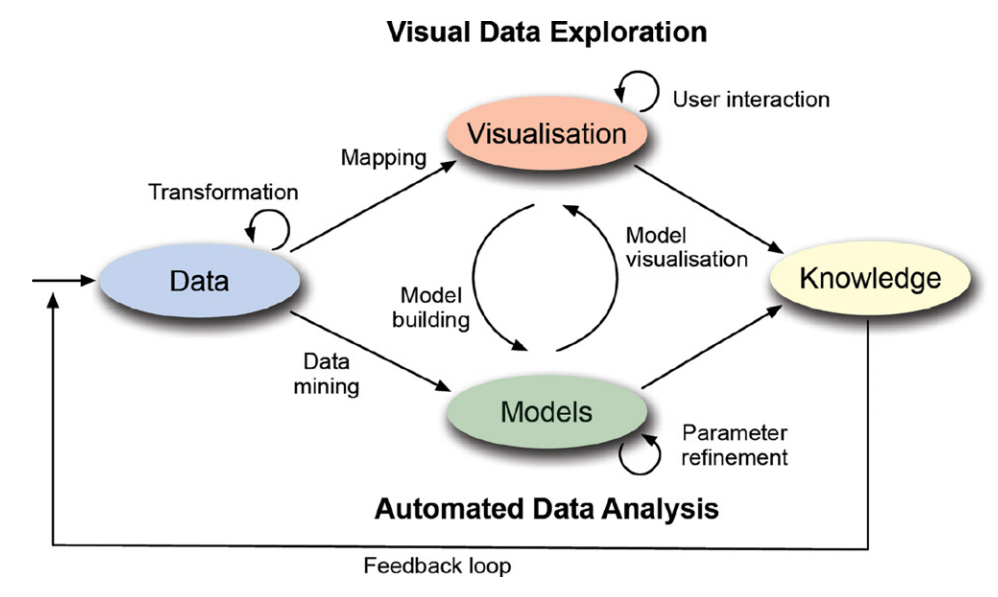
\includegraphics[width=\textwidth]{figures/keim.png}}
	\caption{Visual Analytics Framework, \citep{keim2008visual}}
	\label{keim}
\end{figure}

Visualizing a network graph can be done in two primary ways: node-link diagrams and adjacency matrices. The most familiar visualization is the node-link diagram . \cite{ghoniem2004comparison} considers the two different representation and compares the readability of the two graphs. Although the international trade network starts out with a large number of nodes, when filtering is applied \citep{shneiderman1996eyes} it has a limited number of nodes. Therefore when choosing the appropriate visualization I consider it a small graph, and node-link diagrams are more readable \citep{ghoniem2004comparison}.\par
Node placement is a consideration when network visualization is concerned. A common layout strategy is based on geographic representation \citep{shneiderman2006network}. This geographically representative positioning is used in both of the main visual representations. The linked multiple views of the familiar world map (choropleth) and the network visualization allow for a greater understanding \citep{rodgers2005graph}.\par
When visualizing a network minimizing edge crossing is the most important aesthetic consideration \citep{purchase1997aesthetic} for improving human comprehension. A number of different algorithms for graph visualization were reviewed (\cite{herman2000graph}, \cite{dunne2013motif}, \cite{holten2009force}) that help with this consideration. \cite{herman2000graph} overviews a number of basic graph layout algorithms in the context of information visualization. \cite{dunne2013motif} offers a technique to simplify highly clustered network graphs by aggregating subnetworks. Simplifying the drawing of certain types of motifs can greatly increase readability in dense network graphs. \cite{holten2009force} shows another example of a technique aimed at simplifying complex network graphs. This is achieved by bundling of similarly drawn edges and subsequent splitting of the edges closer to the termination node. Ultimately these algorithms were removed from consideration in favor of mental mapping \citep{eades1991preserving}. Nodes were positioned approximately geographic to aid in the establishment of this mental map. The minimization of edge crossing is accomplished interactively by dragging of nodes after a simulation baseline is established.\par
Effective human computer interaction is an important piece in any visual analytics system. The network visualization is a overview representation of the food trade network. Zooming and filtering is accomplished with uniform scaling in order to preserve the mental map \citep{eades1991preserving}.



Visualization is only only one part of a visual analytics system, knowledge is the end goal. \cite{keim2008visual} states the challenge is to identify the best automated algorithm for the analysis task at hand, identify its limits which can not be further automated, and then develop a tightly integrated solution with adequately integrates the best automated analysis algorithms with appropriate visualization and interaction techniques\par




Effective human computer interaction is an important piece in any visual analytics system. The network visualization is a overview representation of the food trade network. Zooming and filtering is accomplished with uniform scaling in order to preserve the mental map \citep{eades1991preserving}.



Visualization is only only one part of a visual analytics system, knowledge is the end goal. \cite{keim2008visual} states the challenge is to identify the best automated algorithm for the analysis task at hand, identify its limits which can not be further automated, and then develop a tightly integrated solution with adequately integrates the best automated analysis algorithms with appropriate visualization and interaction techniques\par













	After identifying a country and trade good exploration will continue further with the geospatial, line graph and network graph visualizations to determine the extent of the trade network impact for this particular parameter selection. After executing a simulation users are able to immediately see the downstream secondary and tertiary effects on the trade network. Actual trade link effects (network graph link size changes), triadic significance profile deviations (line graph) and vulnerability measures (choropleth) are available as a visualization in the dashboard. Through the feedback loop \citep{keim2006challenges} the results are refined by consecutive iterations.\par



	A base vulnerability index (choropleth) is provided to the user and domain-experts can make further determinations as to the vulnerability of the identified country based on other factors such as governance or economic health of the country that is outside the scope of this thesis. The model can then be manipulated to further explore if a climate singularity would have a measurable impact on the world agricultural trade network. Using data and previous research domain-experts will be able determine a subset of agricultural goods and countries which are vulnerable to a particular climate event based on these predictions.\par

%-----------------------back matter
{\singlespace
% Making the references a "part" rather than a chapter gets it indented at
% level -1 according to the chart: top of page 4 of the document at
% ftp://tug.ctan.org/pub/tex-archive/macros/latex/contrib/tocloft/tocloft.pdf
\addcontentsline{toc}{part}{REFERENCES}
%\nocite{*}
\bibliographystyle{asudis}
\bibliography{thesis}
}
%\renewcommand{\chaptername}{APPENDIX}
%\addtocontents{toc}{APPENDIX \par}
%\appendix
%\chapter{RAW DATA}

%\include{vita}
\end{document}
